\documentclass[12pt,a4paper,english]{article}
%\usepackage[latin1]{inputenc}
\usepackage[utf8]{inputenc}

% Latex report template for The Norwegian Meteorological Institute
% Updated 2015-06-25 by Oskar Landgren, oskar.landgren@met.no
% Edit as you wish, but please report if you find any errors.
% The old template has been circulating in many different versions,
% so you may have more clever implementations for certain
% applications. Improvement suggestions are welcome!
% 
% Update history:
% 2015-06-25 - More bug fixes. Works without interruption either directly from pdflatex
%              or by using latex and dvipdf. A few "Overfull \hbox" errors are normal.
%              (The DVI file does not show correct font in Ubuntu Document Viewer,
%              but is correct after conversion to PDF.)
% 2015-02-16 - Minor fixes (e.g. now using \providecommand{\cftchapfont} instead of renewcommand{....})
% 2015-02-04 - Heading font changed to Arial/Helvetica while keeping main text in Times New Roman.
% 2014-11-17 - Font changed to Times New Roman.
% 2014-11-10 - Minor fixes, plus added a few comments about how to assign affiliations for authors.
% 2013-06-28 - Thanks to Lars-Petter Røed for adding various useful packages. (Comments beginning with "LPR:")
% 2013-06-18 - Added agufull04.bst and PDF versions of logo for pdftex users. Thanks to Magne Simonsen.

%%% For debugging, use
% \errorcontextlines 10000

\usepackage[english]{babel}

%%% LPR: Changed graphic package. Note that pstricks is in conflict with package xcolor
%\usepackage{graphicx}
\usepackage{epsfig}            % To allow figures
\usepackage{pstricks}          % To draw color pictures directly

%\usepackage{pstcol,pst-grad}   % To construct pictures directly
%\usepackage{pst-node,pst-plot} % To construct pictures directly
\usepackage{graphics}

\usepackage{supertabular}
\usepackage{longtable}
\usepackage{multicol}

\usepackage{fancyhdr}
\usepackage[verbose,a4paper,tmargin=30mm,bmargin=37.5mm,lmargin=30mm,rmargin=30mm]{geometry}

%%% OL: The new visual identity uses Arial as header font. It is not a free font so it may not be included in your Linux installation.
%       You may use the uarial package, which can be installed by running the following command in your terminal: sudo getnonfreefonts-sys -a
%       Since it may not be possible to use for everyone (e.g. if you do not have permissions to run the command above),
%       another similar sans-serif font is Helvetica, which should be installed by default.
%\usepackage{uarial}
\usepackage{helvet}

%\usepackage{times}   % OL: Older version of Times font.
\usepackage{mathptmx} % OL: Times New Roman, including math symbols.
\usepackage[T1]{fontenc}

% Arial was previously used in main text, but last version has gone back to Times New Roman.
% Required lines for replacing the main font:
%\renewcommand{\familydefault}{\sfdefault}
%\renewcommand{\rmdefault}{phv}
%\renewcommand{\sfdefault}{phv}

\usepackage{rotating}

%%% LPR: Packages amssymbol and amsmath added to make use of extended
%        special and mathematical characters, e.g., bold greek letters        
\usepackage{amssymb}       % More special characters          
\usepackage{amsmath}       % More mathematical characters

%%% LPR: Package natbib added to ease referencing. Remember to 
%        specify the pathway where to find the bib-file (the file
%        containing the references) at the location where you wish the
%        the reference chapter to appear (see end of this file).
\usepackage{natbib} % Needed e.g. for \citep

%%% OL: These packages were used before, but I could not find them in my TeX installation.
%\usepackage{publication} 
%\usepackage{tellus} 

%%% LPR: The package multirow added to allow for multiple rows
\usepackage{multirow}

%%% LPR: Package verbatim added to allow use of comment environment, that is,
%        to allow use of \begin{comment} and \end{comment}
\usepackage{verbatim}          % Use the verbatim styles

%%% LPR: Package dcolumn added to help align entries in tables
\usepackage{dcolumn}

\definecolor{METblue}{cmyk}{0.85,0,0.2,0.2}

%%% Putting the section numbers in the left margin using package titlesec
%   More info at http://texdoc.net/texmf-dist/doc/latex/titlesec/titlesec.pdf
\usepackage{titlesec}

% Titleformat syntax: \titleformat{command}[shape]{format}{label}{sep}{before-code}[after-code]
\titleformat{\section}
  [block]
  { \normalfont\sffamily\Large\bfseries\color{METblue} }
  {\makebox[2em][r]{\thesection}}
  {5mm}
  {\vspace{5mm}}

\titleformat{\subsection}[block]%
  {\normalfont\sffamily\bfseries}%
  {\makebox[2em][r]{\thesubsection}}%
  {5mm}
  {\vspace{3mm}}[]
\titleformat{\subsubsection}[block]%
  {\normalfont\sffamily\bfseries}%
  {\makebox[3em][r]{\thesubsubsection}}%
  {5mm}
  {\vspace{3mm}}[]

% Titlespacing syntax: \titlespacing*{command}{left}{before-sep}{after-sep}[right-sep]
\titlespacing*{\section}{-17mm}{5mm}{0mm}
\titlespacing*{\subsection}{-13.5mm}{5mm}{0mm}
\titlespacing*{\subsubsection}{-17.5mm}{5mm}{0mm}

%%% Formatting the table of contents
\usepackage{tocloft}
\renewcommand{\cfttoctitlefont}{\sffamily\bfseries\color{METblue}\Large}
\providecommand{\cftchapfont}{\sffamily\bfseries }
\renewcommand{\cftsecfont}{\sffamily\bfseries }
\renewcommand{\cftsubsecfont}{\sffamily }
\renewcommand{\cftsubsubsecfont}{\sffamily }
\providecommand{\cftsubsubsubsecfont}{\sffamily }
\renewcommand{\cftfigfont}{Figure }
\renewcommand{\cfttabfont}{Table }
\providecommand{\cftchappagefont}{\sffamily}
\renewcommand{\cftsecpagefont}{\sffamily\bfseries}
\renewcommand{\cftsubsecpagefont}{\sffamily}
\renewcommand{\cftsubsubsecpagefont}{\sffamily}
\providecommand{\cftsubsubsubsecpagefont}{\sffamily}

%\listfiles
\renewcommand{\baselinestretch}{1.33}
% \geometry{verbose,a4paper,tmargin=20mm,bmargin=20mm,lmargin=30mm,rmargin=30mm}

%%% OL: If your authors need different affiliations you may use one of the following solutions:
% "authblk", http://tex.stackexchange.com/questions/9594/adding-more-than-one-author-with-different-affiliation
% "revtex", http://tex.stackexchange.com/questions/5805/revtex-4-1-multiple-affiliations
% or redefine the author command using http://tex.stackexchange.com/questions/107739/authors-with-multiple-affiliations

%% LPR: These are my favorite definitions and abbreviations. Just add or delete as you see fit for your purpose
% Definitions:
% 1. Often repeated stuff
\def\DR{Dr{\o}bak}
\def\HAA{H{\aa}{\o}ya Island}
\def\wrt{with respect to}
\def\hhv{respectively}
\def\fe{for instance}
\def\dvs{that is}
\def\metno{Norwegian Meteorological Institute}
\def\swe{shallow water equations}

% 2. Mathematical stuff: 
% 2.1 Equations:
\def\be{\begin{equation}}
\def\ee{\end{equation}}
\def\beq{\begin{eqnarray}}
\def\eeq{\end{eqnarray}}
\def\bfig{\begin{figure}}
\def\efig{\end{figure}}
\DeclareMathOperator{\sgn}{sgn}
% 2.2 Differentiation:
\def\pt{\partial_t}
\def\px{\partial_x}
\def\py{\partial_y}
\def\pz{\partial_z}
\def\ptt{\partial_t^2}
\def\pxx{\partial_x^2}
\def\pyy{\partial_y^2}
\def\pzz{\partial_z^2}
\def\pts{\partial_{t'}}
\def\pxs{\partial_{x'}}
\def\pys{\partial_{y'}}
\def\pzs{\partial_{s}}
\def\dels{\nabla_{s}}
% 2.3 Numerical time step and grid steps:
\def\Dx{\Delta x}
\def\Dy{\Delta y}
\def\Dz{\Delta z}
\def\Dt{\Delta t}
\def\Ds{\Delta s}
% 2.4 Vectors:
\def\vec{\mathbf}
\def\bu{\mathbf{u}}
\def\bv{\mathbf{v}}
\def\bi{\mathbf{i}}
\def\bj{\mathbf{j}}
\def\bk{\mathbf{k}}
\def\bU{\mathbf{U}}
\def\bV{\mathbf{V}}
\def\ud{\textrm{d}}
% 2.5 Convenient abbrivations
\def\th{\theta}
\def\bhu{\vec{\bar{u}}}
\def\hu{\bar{u}}
\def\hv{\bar{v}}
\def\hp{\bar{\phi}}
\def\ha{\hat{a}}
\def\hb{\hat{b}}
\def\hc{\hat{c}}
\def\hC{\bar{C}}
\def\hd{\hat{d}}
\def\he{\hat{e}}
\def\hf{\hat{f}}
\def\hg{\hat{g}}
\def\mc{\multicolumn}
% 8. Sigma coordinate derivatives
\def\ptg{\partial_{t'}}
\def\pxg{\partial_{x'}}
\def\pyg{\partial_{y'}}
\def\pzg{\partial_{\sigma}}
\def\delg{\nabla_{\sigma}}
% 2.6 Operators
\def\del{\nabla_H}
\def\dels{\nabla_s}
\def\eps{\epsilon}
\def\vphi{\varphi}
\def\matO{\mathcal{O}}
\def\matG{\mathcal{G}}
\def\matH{\mathcal{H}}
% 2.7 Tensors
\def\mat{\boldsymbol}
\def\matI{\boldsymbol{\mathcal{I}}}
\def\matA{\boldsymbol{\mathcal{A}}}
\def\matB{\boldsymbol{\mathcal{B}}}
\def\matC{\boldsymbol{\mathcal{C}}}
\def\matD{\boldsymbol{\mathcal{D}}}
\def\matM{\boldsymbol{\mathcal{M}}}
\def\matE{\boldsymbol{\mathcal{E}}}
\def\matF{\boldsymbol{\mathcal{F}}}
\def\matL{\boldsymbol{\mathcal{L}}}
\def\matU{\boldsymbol{\mathcal{U}}}
\def\matV{\boldsymbol{\mathcal{V}}}
\def\matK{\boldsymbol{\mathcal{K}}}

% 3. Specialties 

% End LPR definitions
%%%%%%%%%%%%%%%%%%%%%%%%%%%%%%%%%%%%%%%%%%%%%%%%%%%%%%%%%%%%%%%%%%%%%%%

% --------------------------------------

\begin{document}

%%%%%%%%%%%%%%%%%%%%%%%%%%%%%%%%%%%%%%%%%%%%%%%%%%%%%%%%%%%%%%%%%%%%%%%
% Specify path to bibliography style
\bibliographystyle{/home/larspr/LATEX/bst-files/agufull04}
%%% LPR: Note that you must give the path to the directory of your reference file (*.bib file). See the end of this file
 
%%%%%%%%%%%%%%%%%%%%%%%%%%%%%%%%%%%%%%%%%%%%%%%%%%%%%%%%%%%%%%%%%%%%%%%
% Specify graphics path (where to find the figures). Automatically chooses PDF or EPS depending on latex (EPS) or pdflatex (PDF).
\graphicspath{{./GRAPHICS/}} 

\pagenumbering{roman} % Use roman numerals for page numbering before main content. OL: The new template begins with page 1 on the cover.
\thispagestyle{empty}  % Hide page numbers

\noindent
\begin{tabular}{@{} p{63mm} p{50mm} r}
\includegraphics*[]{met_rapport_logo_eng} % Automatically uses PDF or EPS depending on latex (EPS) or pdflatex (PDF).
&
\fontsize{27.5pt}{33pt} \selectfont \bf \sffamily MET{\color{gray} report}
&
 \begin{minipage}[b]{28mm}
  \begin{flushright}
   \footnotesize \sffamily No. X/2015 \\ ISSN 2387-4201 \\ Oceanography	% Report number and Category
  \end{flushright}
 \end{minipage}
\end{tabular}

\vfill

%%% LPR: Note that the ratio between the two numbers in \fontsize{a}{b} below must be such that b/a = 1.2
\begin{flushright}
{\fontsize{20pt}{24pt}\selectfont \bf \sffamily A high-resolution, curvilinear version of ROMS for the Oslofjord}	% Title

{\fontsize{14.0pt}{16.8pt}\selectfont \bf \sffamily FjordOs technical report No. 2% Subtitle
%%% LPR: Changed from \vspace{5mm}
\vspace{5mm}	% \vspace{5mm}
\\

\sffamily Lars Petter R{\o}ed, Nils Melsom Kristensen, \\Karina Bakkel{\o}kken Hjelmervik and André Staalstr{\o}m	% Author name(s)
}
\end{flushright}

%\vspace{25mm}
\vspace{2mm}

\begin{figure}[!h]
 \begin{center}
%% LPR: The original MET_report template command 
%\includegraphics*{met_rapport_monster} 
%% is replaced by:
  {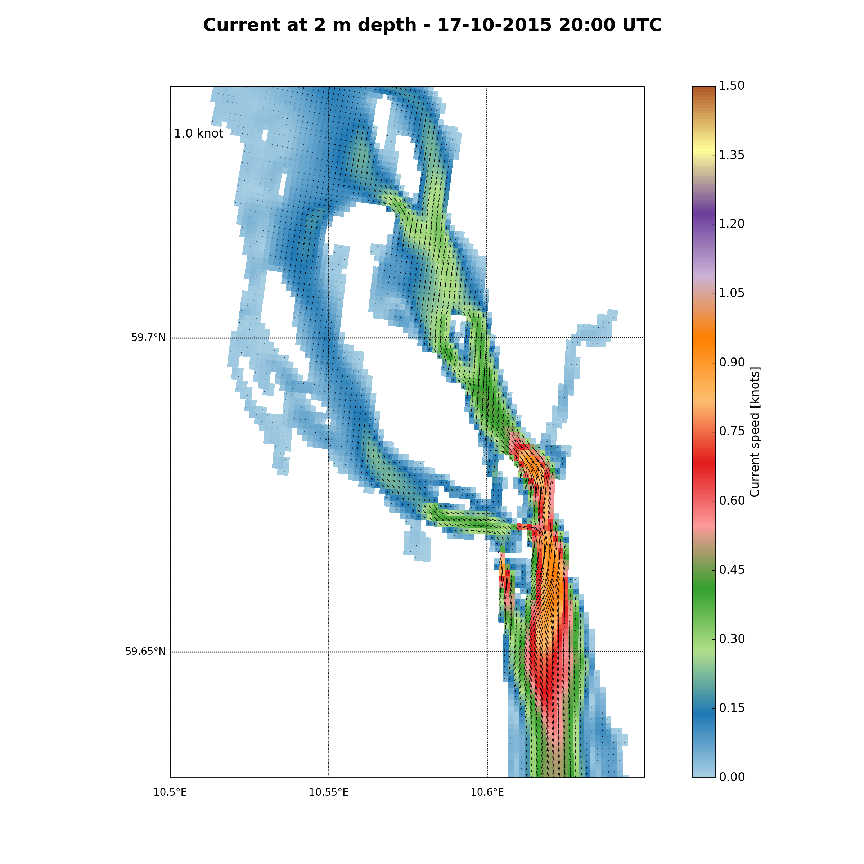
\includegraphics[height=13cm]{droebak_current_2015-10-17_20UTC}}	% Graphic. Automatically uses PDF or EPS in same directory depending on latex or pdflatex.
 \end{center}
\end{figure}

%\newpage


\clearpage
\thispagestyle{empty}  % Hide page numbers

\setlength{\unitlength}{1mm}  %Needed for picture environment

\begin{table}[!ht]

\begin{tabular}[c]{lr}
\vspace{5mm}
\includegraphics*{met_rapport_logo_eng} & \hspace{43mm}
{\fontsize{27.5pt}{33pt}\selectfont \bf \sffamily MET{\color{gray} report}}\\
\end{tabular}

\sffamily{
\begin{tabular}[t]{|p{110mm}|p{40mm}|} \hline
{\bf \sffamily Title}                  & {\bf \sffamily Date}               \\ 
\small{A high-resolution, curvilinear version of ROMS for the Oslofjord: FjordOs technical report No. 2}
                             & \today                   \\ \hline
{\bf \sffamily Section}                & {\bf \sffamily Report no.}         \\ 
 Ocean and Ice                         &  4/2016                  \\ \hline
{\bf \sffamily Author(s)}                 & {\bf \sffamily Classification}     \\ 
\small{Lars Petter R{\o}ed, Nils Melsom Kristensen, Karina Bakkel{\o}kken Hjelmervik, André Staalstr{\o}m}                
                             & \begin{picture}(20,4)(-2,-1.0)
                               \put (0,0){\circle*{4}}
                               \put (7,0){\makebox(0,0){Free}}
                               \put (15,0){\circle{4}}
                               \put (27,0){\makebox(0,0){Restricted}}
                               \end{picture}
                               \\ \hline
{\bf \sffamily Client(s)}              & {\bf \sffamily Client's reference} \\ 
Client name                  &               \\ \hline
\end{tabular}

\begin{tabular}[t]{|p{154.3mm}|}
{\bf \sffamily Abstract}                                          \\
\small{Provided is a detailed documentation of a new Oslofjord model, FjordOs CL, utilizing the curvilinear option of the Regional Ocean Modeling System - ROMS. The development is part of the project FjordOs. FjordOs CL has a spatial grid size varying from about 50 meters in the {\DR} sound to about 300 meters at its southern open boundary bordering on the Skagerrak. It features 42 terrain-following levels in the vertical. It is forced by atmospheric as well as river and tidal input in addition to input at its lateral open boundary. The atmospheric input is from MET Norway's operational NWP model (AROME-MetCoOp). River input is via 37 rivers based on NVE's hydrological model and discharge observations. Ocean input is from MET Norway's operational, ocean forecasting model NorKyst800. The tidal input is based on the TPXO Atlantic database modified by observations and provides nine tidal constituents as input.
 } 
%bla bla
	% Abstract text...
%\\[50mm] % Add whitespace if necessary
\\ \hline
{\bf \sffamily Keywords}                                          \\ 
  \small{Ocean model, Numerical methods, Oslofjord}    \\ 
\hline
\end{tabular}
}

\begin{tabular}[t]{cc}
					&			\\
					&			\\
					&			\\
\line(1,0){70}				& \line(1,0){70}	\\ 
\small{Disciplinary signature}		& \small{Responsible signature}	\\
\small{Kai H. Christensen}		& \small{Lars Anders Breivik}	\\       % Add names if needed
\hspace{75mm}				& \hspace{75mm}		\\

\end{tabular}
\end{table}

\clearpage


\thispagestyle{empty} % Hide page numbers
\newpage
\thispagestyle{fancy} % footer from fancyhdr package
\headheight=15pt
\renewcommand{\headrulewidth}{0pt}

\section*{\hspace{17mm}Abstract}
Provided is a detailed documentation of a new Oslofjord model, FjordOs CL, utilizing the curvilinear option of the Regional Ocean Modeling System - ROMS. The development is part of the project FjordOs. FjordOs CL has a spatial grid size varying from about 50 meters in the {\DR} sound to about 300 meters at its southern open boundary bordering on the Skagerrak. It features 42 terrain-following levels in the vertical. It is forced by atmospheric as well as river and tidal input in addition to input at its lateral open boundary. The atmospheric input is from MET Norway's operational NWP model (AROME-MetCoOp). River input is via 37 rivers based on NVE's hydrological model and discharge observations. Ocean input is from MET Norway's operational, ocean forecasting model NorKyst800. The tidal input is based on the TPXO Atlantic database modified by observations and provides nine tidal constituents as input.
	% Abstract text...

%\vfill

\fancyfoot{
% If abstract on separate page is not needed, move the following table to the page before
\begin{tabular}[b]{p{40mm}p{25mm}p{25mm}p{25mm}p{25mm}}
 \begin{minipage}[l]{40mm} \tiny \color{METblue} {\bf Norwegian Meteorological Institute}\\ Org.no 971274042\\ post@met.no\\ www.met.no / www.yr.no
 \end{minipage} & 
 \begin{minipage}[l]{25mm} \tiny \color{METblue} {\bf Oslo}\\ P.O. Box 43, Blindern\\ 0313 Oslo, Norway\\ T. +47 22 96 30 00
 \end{minipage} &
 \begin{minipage}[l]{25mm} \tiny \color{METblue} {\bf Bergen}\\ All\'egaten 70\\ 5007 Bergen, Norway\\ T. +47 55 23 66 00
 \end{minipage} & 
 \begin{minipage}[l]{25mm} \tiny \color{METblue} {\bf Troms\o}\\ P.O. Box 6314, Langnes\\ 9293 Troms\o, Norway\\ T. +47 77 62 13 00
 \end{minipage} & 
 \begin{minipage}[l]{25mm} \tiny \color{METblue} 
 \end{minipage}
\end{tabular}
}

%\thispagestyle{empty} % Hide page numbers
\clearpage
%\thispagestyle{empty} % Hide page numbers
\tableofcontents

\clearpage
%%%%%%%%%%%%%%%%%%%%%%%%%%%%%%%%%%%%%%%%%%%%%%%%%%%%%%%%%%%%%%%%%%%%%%%
% Set page style to 'plain' and page numbers to arabic digits (starts on 1)
%\newpage
\pagestyle{plain}
\pagenumbering{arabic}

%% Start with and introductory chapter with possible subsections and subsubsections
%%%%%%%%%%%%%%%%%%%%%%%%%%%%%%%%%%%%%%%%%%%%%%%%%%%%%%%%%%%%%%%%%%%%%%%%%%%%%
\section{Introduction}
\label{sec:intro}
Provided is a documentation of a recently developed Oslofjord model called FjordOs CL. It is developed as part of the project FjordOs\footnote{\texttt{http://www.fjordos.no}}. FjordOs CL is based on version 3.6 of the Regional Ocean Modeling System - ROMS \citep{haidv:etal:2008, shche:mcwil:2005, shche:mcwil:2009} utilizing its curvilinear option.

\subsection{The Oslofjord}
\label{subsec:oslofjord}
The Oslofjord is located in Southern Norway and is about 100 km long (Figure \ref{fig:map_oslofj}). Its width varies from about 25 km at the entrance ($\sim$ 59$^\text{o}$N) to about 1-2 km in the {\DR} Sound and {\DR} area. The fjord's main sill, which is marked by the horizontal bar in Figure \ref{fig:map_oslofj} (hereafter the {\DR} Sill), is located two thirds inside of the entrance to the fjord. This makes the Oslofjord peculiar among Norwegian fjords in that most of them have the sill at the entrance to the fjord. 
% %%%%%%%%%%%%%%%%%%%%%%%%%% Figure Map_location_Oslofjord %%%%%%%%%%%%%%%%%%%%%%%%%%%%
\begin{figure}[h]
 \setlength{\unitlength}{1.0cm}
 \begin{center}
  \begin{pspicture}(0,0)(15,9)
% Include graphs
   \rput[bl](-0.1,1.0){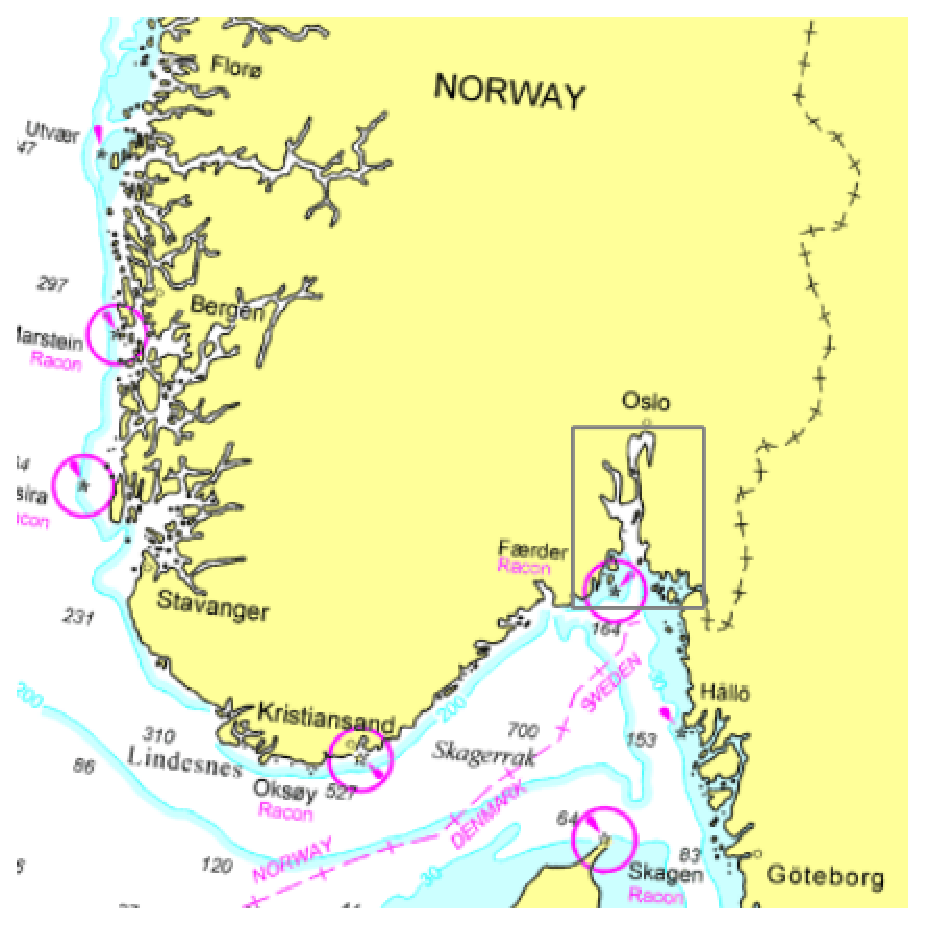
\includegraphics[height=7.3cm]{Map_location_Oslofjord_2}}
   \rput[br](15.0,0.0){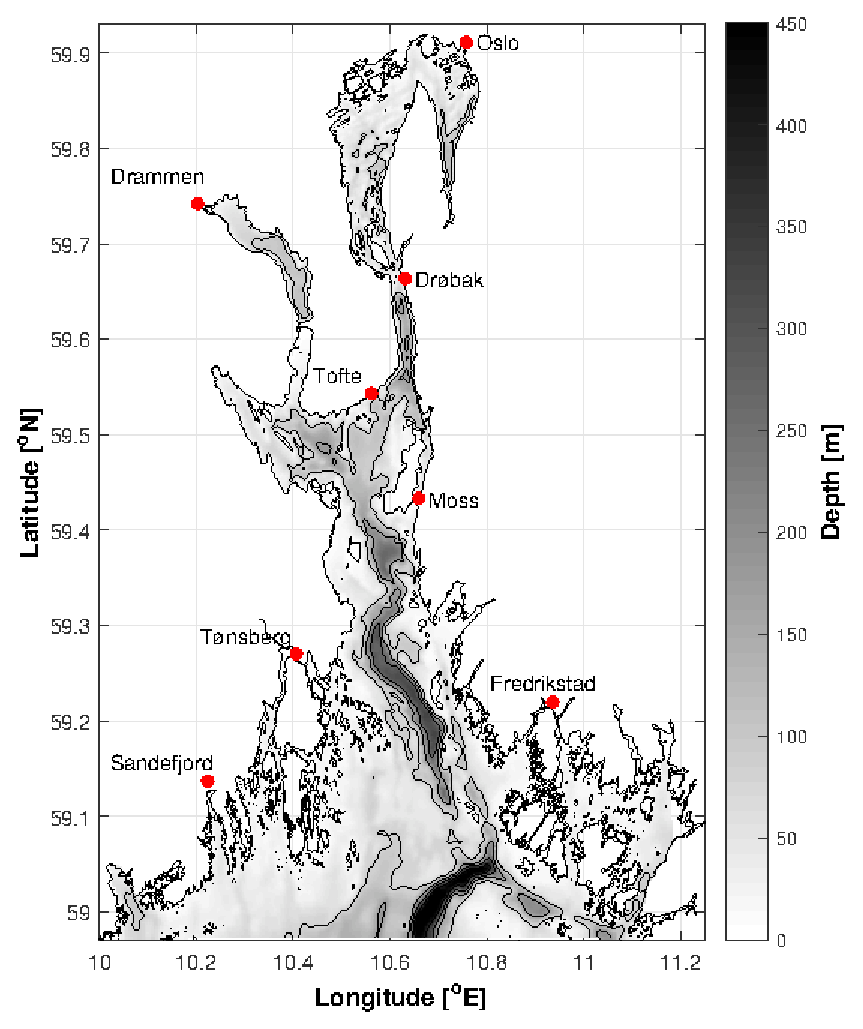
\includegraphics[height=9cm]{dyp_old}}
   \psline[linewidth=0.5mm,linecolor=blue]{->}(13.4,5.3)(11.3,6.3)
   \psline[linewidth=0.2mm](4.45,4.95)(7.5,8.5)
   \psline[linewidth=0.2mm](4.45,3.5)(7.5,1)
  \end{pspicture}
% Figure caption is below the figure
  \caption{\small The topography and irregular coastline of the Oslofjord and its location in Southern Norway. The right-hand gray scale bar indicates depth in meters. The blue arrow points to the location of the fjord's main sill (the {\DR} sill as enlarged in Figure \ref{fig:droebak_sill}) which is only $\sim$ 20 m deep. Note also the $\sim$ 400 m deep basin extending from the Skagerrak towards the Hvaler Archipelago in the southeast, the so called Hvalerdjupet. }
  \label{fig:map_oslofj}       % Give a unique label
 \end{center}
\end{figure}
%


The {\DR} Sill is partly man made\footnote{The jetty was built in the years 1874 - 1879 as a naval defense of Oslo, the capital of Norway. It forces large vessels to sail east of the fortress Oscarsborg built at Kaholmen.} and partly natural. The natural sill is about 20 m deep, while the man made part is only 1-2 m deep. The latter consists of an underwater barrier, the {\DR} Jetty, extending halfway across the {\DR} Sound from the western mainland south of {\DR} to south of the small island Kaholmen located slightly to the east of the southern tip of the {\HAA} (Figure \ref{fig:droebak_sill}). There are two narrow openings in the Jetty with a maximum depth of about 6 m. One is located close to the mainland on the western side, while the second runs east-west and is located just south of Kaholmen.   
%%%%%%%%%%%%%%%%%%% Figure 2 Bathymetry and currents in the Drøbak area %%%%%%%%%%%%%%%
\begin{figure}[t]
 \begin{center}
  \begin{pspicture}(0,0)(15,9)
% Include graphs
   \rput[b](7.5,0){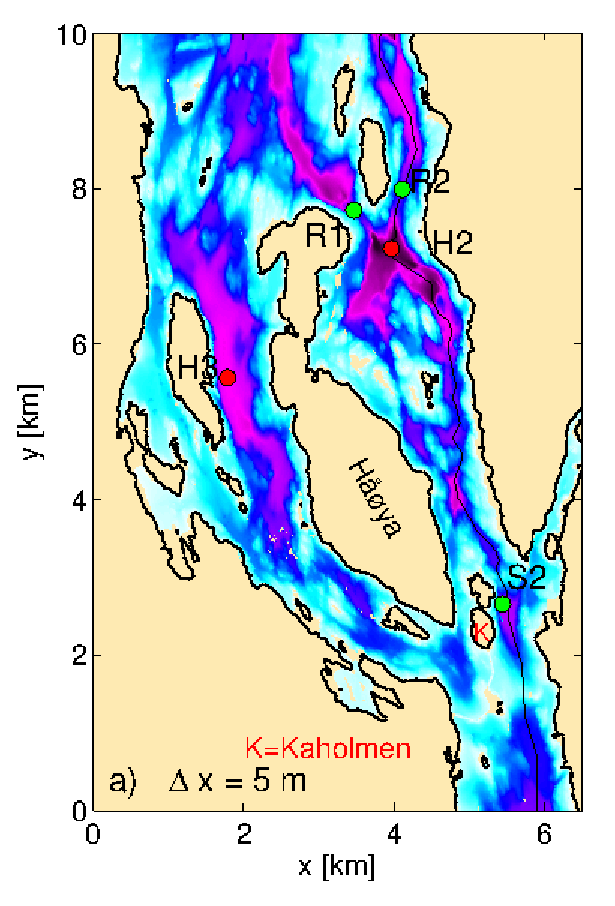
\includegraphics[height=9cm]{dyp_Drobak}}
   \rput[b](11,0){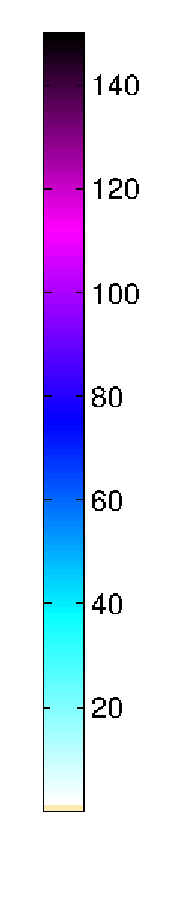
\includegraphics[height=9cm]{Fig02_color_bar}}
  \end{pspicture}
  \caption{\small The irregular coastline and topography in the {\DR} Sill area. The color bar indicates depth in meters.}
  \label{fig:droebak_sill}
 \end{center}
\end{figure}

 

The sill area represent a major obstruction for the water exchange between the inner and the outer part of the fjord. Due its narrowness and shallowness the {\DR} Sill area is famous for its strong tidal currents that easily exceeds 1 m/s. We also note that north of the sill the fjord is separated by {\HAA} into an eastern and a western channel each about 1 km wide. These channels and the openings in the Jetty are important to include in any model of the Oslofjord to obtain realistic circulation patterns and strengths in the area. Another noteworthy topographic feature is the Hvalerdjup located at the entrance to the fjord (Figures \ref{fig:map_oslofj} and \ref{fig:ferder_hvaler}). It is a 400 m deep basin extending northeastward from the Skagerrak towards the Hvaler Archipelago. As revealed by Figure \ref{fig:map_oslofj} there are also several other somewhat shallower basins $\sim$ 150 - 200 m deep as we proceed into the fjord. 
%%%%%%%%%%%%%%%%%%% Figure 2 Bathymetry and currents in the Drøbak area %%%%%%%%%%%%%%%
\begin{figure}[t]
 \begin{center}
  \begin{pspicture}(0,0)(15,8.5)
% Include graphs
   \rput[bl](-0.1,0){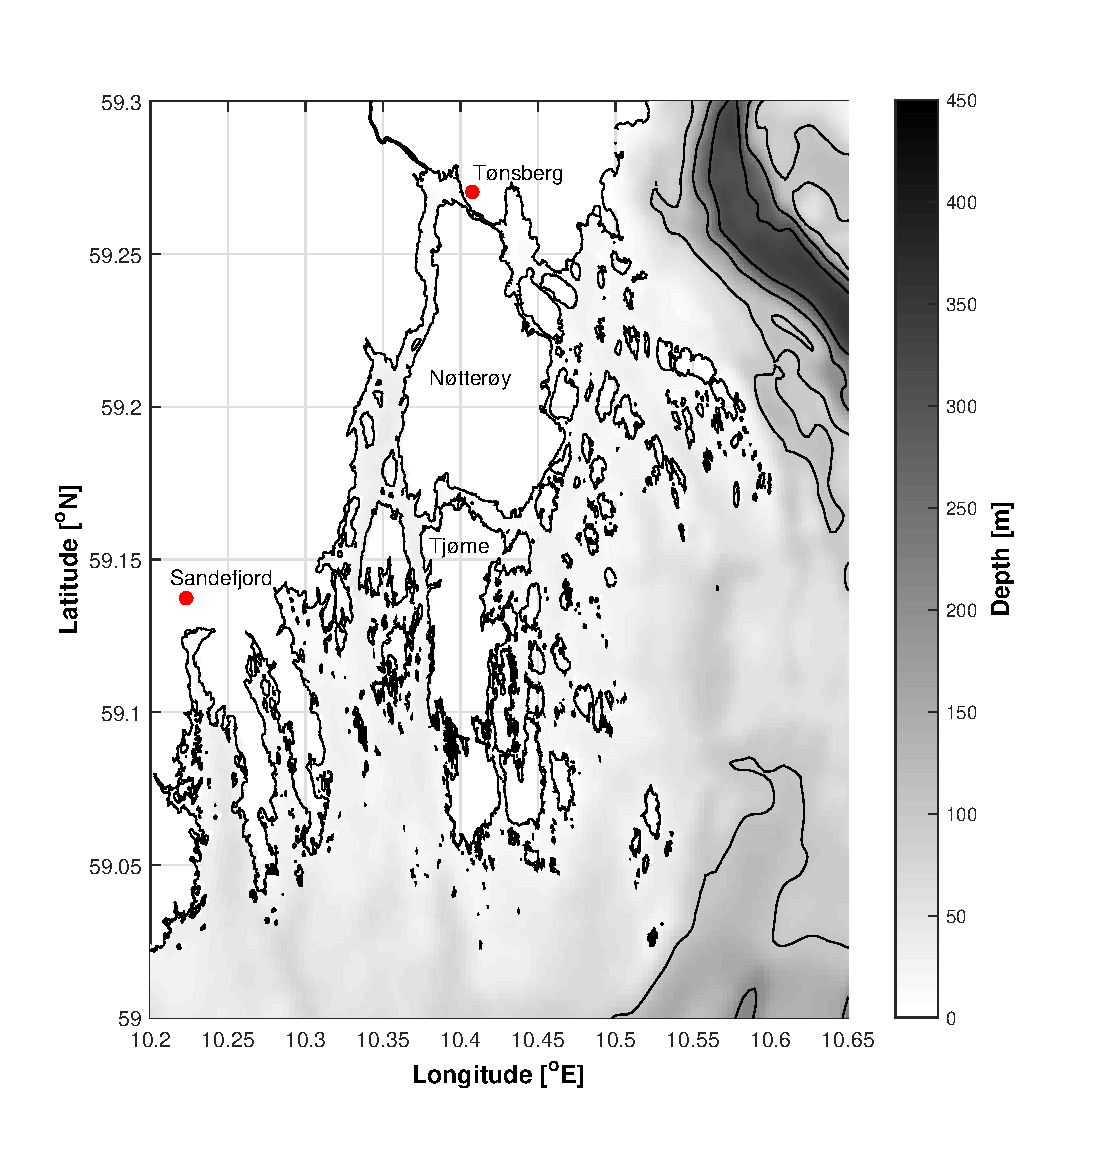
\includegraphics[height=8.5cm]{dyp_Tonsberg}}
   \rput[bl](7.5,0){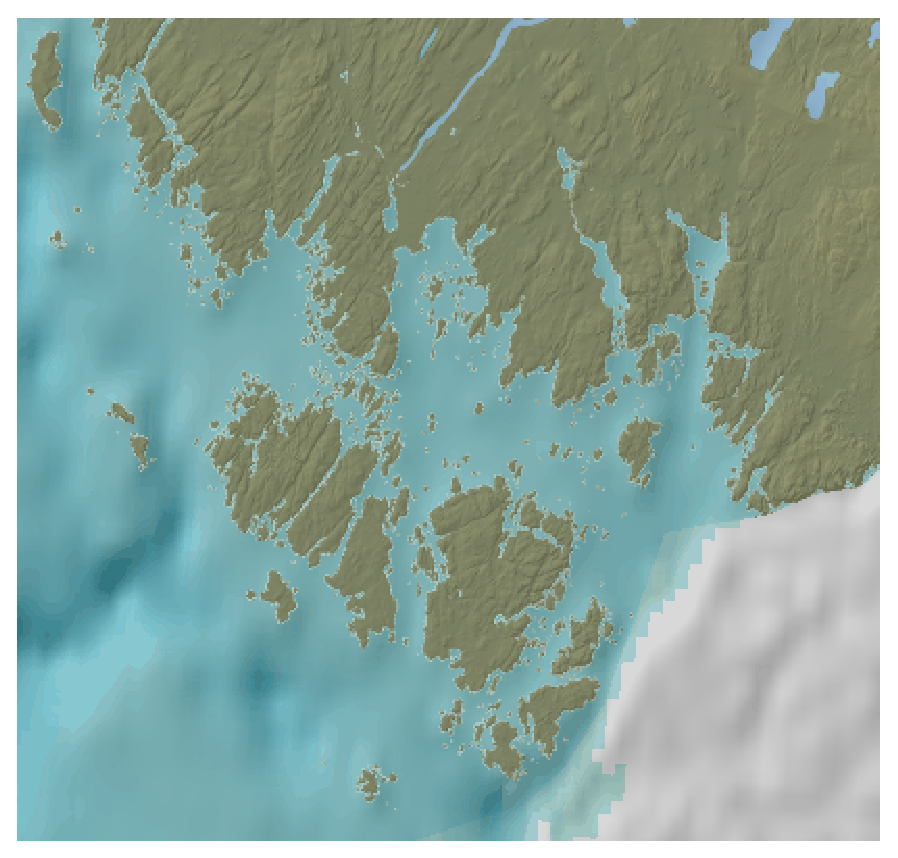
\includegraphics[height=8.5cm]{dyp_Hvaler}}
   \rput[bl](0,7){\large \textbf{a)}}
   \rput[bl](7.5,7){\large \textbf{b)}}
  \end{pspicture}
  \caption{\small a) The irregular coastline geometry and topography in the a) F{\ae}rder National Park and b) the Hvaler National Park. The grayscale in color bars indicates depth in meters. Note the many islands, narrow straits and channels present in these areas of the Oslofjord.}
  \label{fig:ferder_hvaler}
 \end{center}
\end{figure}

 

In addition to the {\DR} Sill area there are other areas in the fjord that features many smaller and larger islands. For instance to the west we find the T{\o}nsberg Archipelago including Bol{\ae}rne, Store and Lille F{\ae}rder (F{\ae}rder Lighthouse), and to the east we find Rauer and Hank{\o}, the Hvaler Archipelago and the smaller Islands S{\o}strene and Misingene (Figure \ref{fig:ferder_hvaler}). Further north on the west side of the fjord we find Bast{\o} south of Horten, and to the east Jel{\o}ya. Jel{\o}ya is separated from the mainland by a narrow channel about 50 m wide within which water sloshes back and forth with the tides \citep{hjelm:etal:2014}. The presence of these archipelagos with its small islands give rise to many narrow sounds, straits and channels impeding the water exchange. If the goal is to compute realistic pathways of any unwanted substances discharged to the fjord or trajectories of floating structures including man overboard (Search and Rescue Services), we need to resolve, to the best of our ability, these features. 

Finally it is worth mentioning the many rivers discharge freshwater to the fjord. For instance two of Norway's largest rivers, namely Glomma and Drammenselva\footnote{Here it is chosen to use Norwegian river names in which ``elv'' or ``vassdrag'', means ``river'' or ``water course''.}, are emptying their freshwater into the Oslofjord with a mean discharge of 729 and 317 m$^3$/s, respectively \citep{milli:etal:2011}. This freshwater has a decisive impact on the salinity and hence on the circulation in the fjord. Furthermore, in most fjords the river outlet is located at the fjord head leading to an estuarine circulation. In contrast the Glomma outlet is located in the outer part of the Oslofjord within the Hvaler Archipelago, while the Drammenselva outlet is located in the middle part of the fjord. As a result the estuarine circulation in the Oslofjord deviates considerably from a classical textbook example.        
%%%%%%%%%%%%%%%%%%%%%%%%%%% Figure 3 Godafoss %%%%%%%%%%%%%%%%%%%%%%%%%%%%%%%
\begin{figure}[t]
 \begin{center}
  \begin{pspicture}(0,0)(15,5.5)
% Include graphs
   \rput[bl](0.0, 0.0){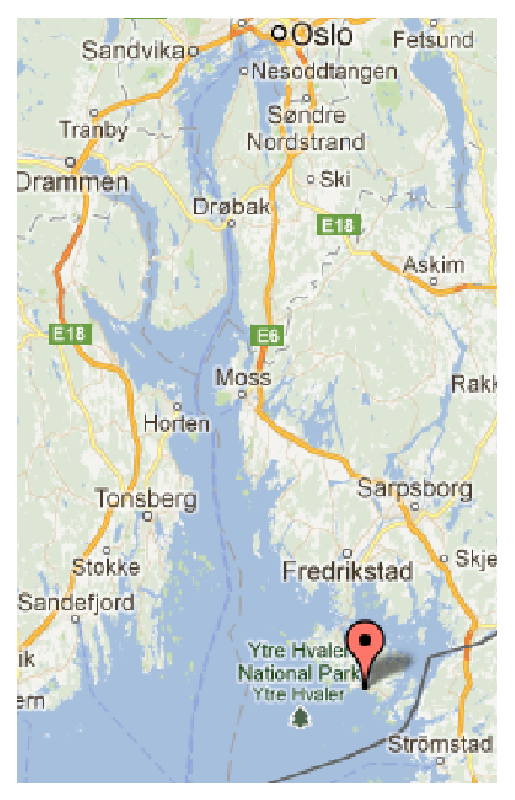
\includegraphics[height=5.5cm]{Fig03}}
   \rput[br](15.0,0.0){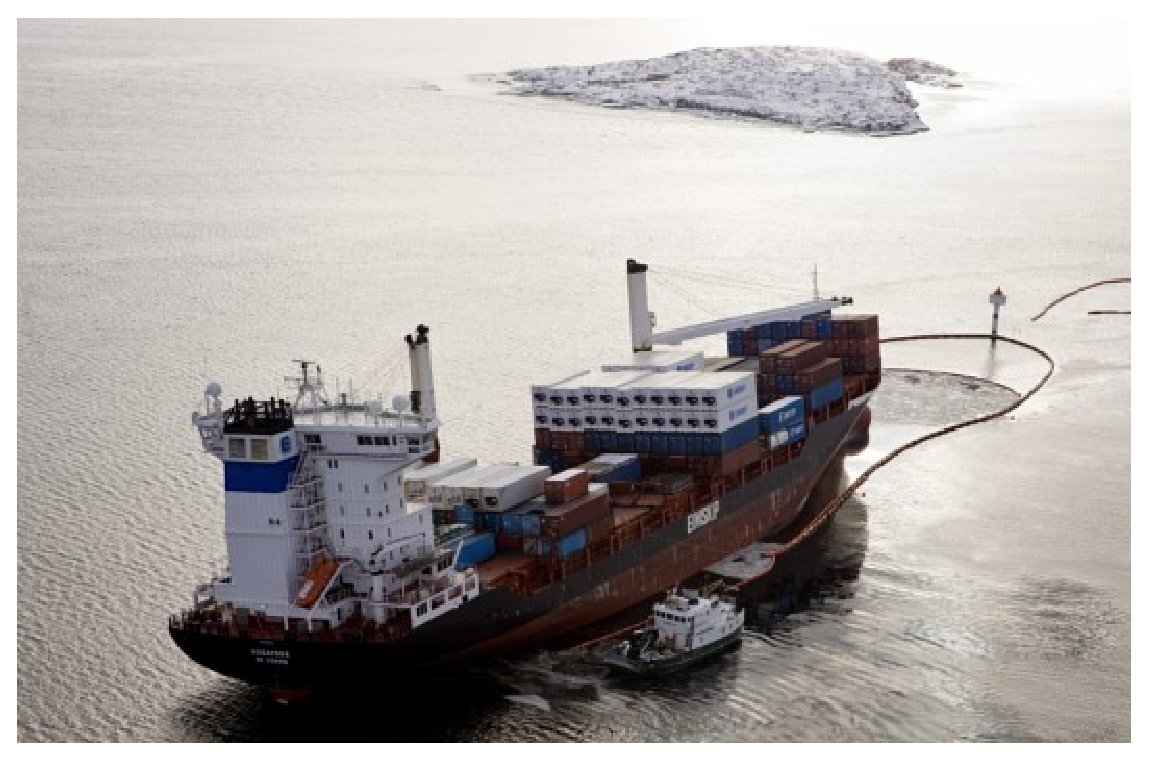
\includegraphics[height=5.5cm]{Fig03_2}}
  \end{pspicture}
  \caption{\small Map (left) showing the location where the ship ``Godafoss'' (right) grounded February 17, 2011. The location is in the sound L{\o}peren between two of the major islands in the Hvaler Archipelago where Norway's largest river flows through on its way to the Oslofjord.} 
  \label{fig:godafoss}
 \end{center}
\end{figure}



% % % % % % % % % % % % % % % % % % % % % % % % % % % % % % % % 
\subsection{Why a new model?}
\label{subsec:why}
The Oslofjord is somewhat special among the Norwegian fjords from a physical as well as a societal perspective. The population surrounding it, or more precisely people living less than one hours drive from the Oslofjord, comprises 40\% of the Norwegian population according to the official statistics\footnote{\texttt{http://www.ssb.no} as of July 1, 2012}. This is by far the most populated area in Norway, a population that is steadily growing. Moreover, no other fjord has anything close to as high density of leisure boats. In addition the Oslofjord features two of Norway's national underwater parks, the Hvaler National Park\footnote{\texttt{http://www.ytrehvaler.no/}} and the F{\ae}rder National Park\footnote{\texttt{http://prosjekt.fylkesmannen.no/faerdernasjonalpark/Om-Farder-nasjonalpark/}}. Thus, taking into account that the Oslofjord has the largest traffic density of commercial vessels of all the Norwegian fjords the risk of an accident resulting in a possible, unwanted contaminated effluent to the fjord is uncomfortably high. 
%%%%%%%%%%%%%%%%%%%%%%%%%%% Figure 3 Godafoss %%%%%%%%%%%%%%%%%%%%%%%%%%%%%%%
\begin{figure}[t]
 \begin{center}
  \begin{pspicture}(0,0)(15,10)
% Include graphs
   \rput[b](7.7, 0.0){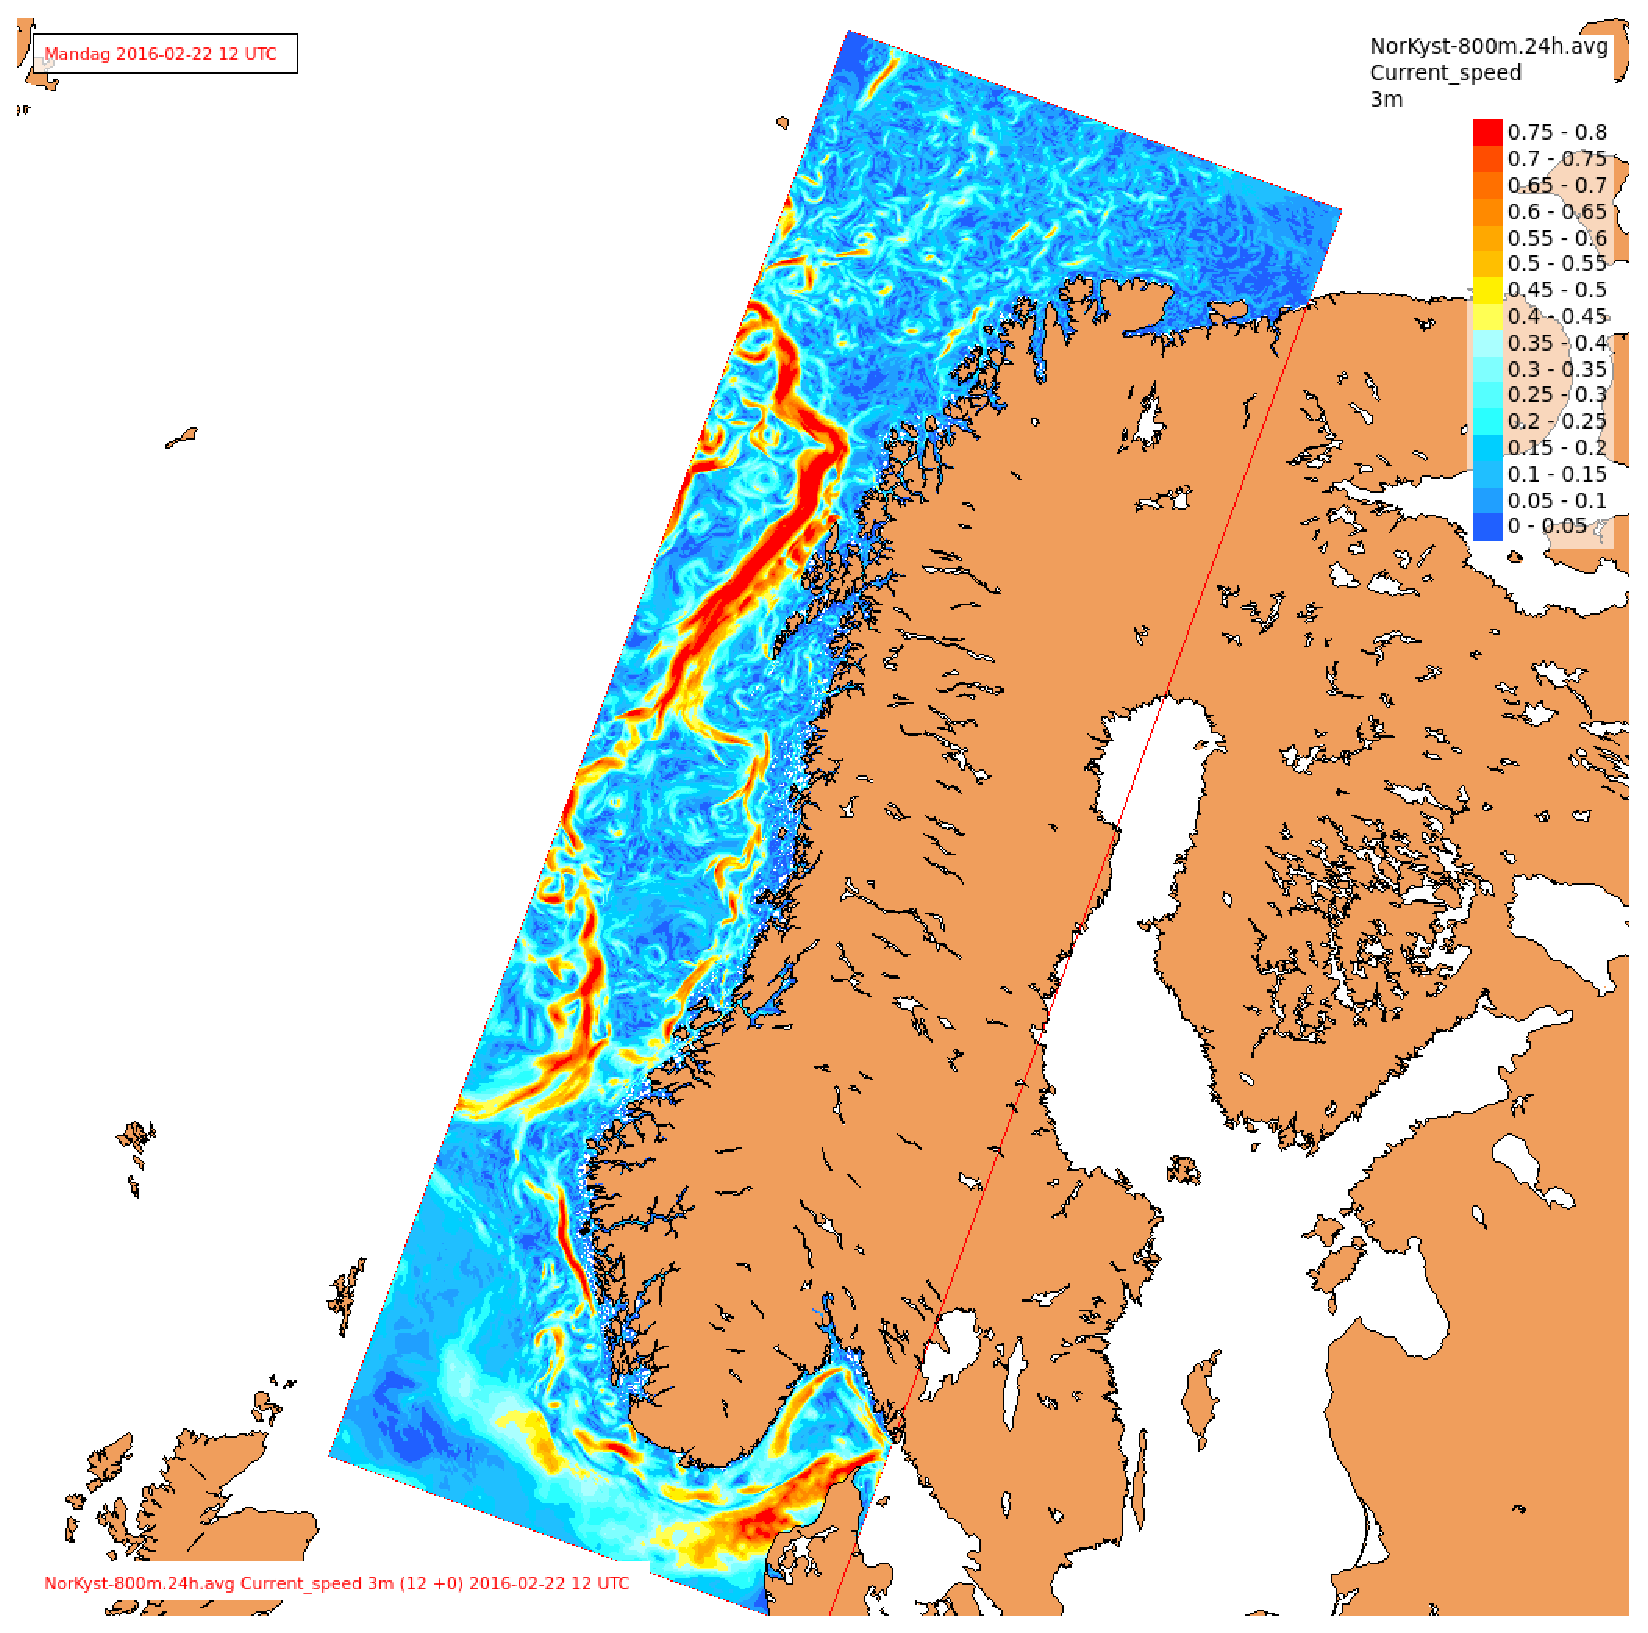
\includegraphics[height=10cm]{N800_2016-02-22_SPEED_3m_24h_avg}}
  \end{pspicture}
  \caption{\small The area covered by the NorKyst800 model. Shown is forecasted, 24 hour average speed at 3 m depth valid for February 22, 2016. Color bar gives speed in m/s with a a contour interval of 0.05 m/s.} 
  \label{fig:n800}
 \end{center}
\end{figure}

 

An example of such an unwanted event is the Godafoss accident. On February 17, 2011 the ship ``Godafoss'' grounded in a narrow sound in the Hvaler Archipelago (Figure \ref{fig:godafoss}), and a lot of its fuel oil leaked into the fjord. As part of the governmental emergency preparedness MET Norway's task is to forecast the dispersion, drift and spreading of the oil no later than half an hour after the accident\footnote{On behalf of the Norwegian Coastal Administration (Kystverket)}. As a matter of fact most of the accidents like Godafoss tend to happen close to the coast or within archipelagos\footnote{\texttt{https://en.wikipedia.org/wiki/List\_of\_oil\_spills}}. The safety of the people that utilize the fjord, and the protection of its environment, is therefore a challenge to governmental agencies, regional administrations and local management alike. 

Together with wind and waves ocean currents and temperature are key inputs to the model used to forecast oil drift. The present forecasting model providing the latter for the Oslofjord, and run operationally by MET Norway, is the NorKyst800 model \citep{albre:etal:2011}. As depicted by Figure \ref{fig:n800} it covers the entire Norwegian coast and not only the Oslofjord. In fact it was not developed to capture details within the Norwegian fjords, but rather to capture mesoscale phenomena such as jet currents, eddies and meanders along the the Norwegian coast outside of the fjords. It was set-up with a regular grid of 800x800 m, a grid of high  enough resolution to resolve the Rossby radius of deformation required to capture the mesoscale phenomena in Norway's near coastal waters. Nevertheless, due to its relatively high resolution of 800 m, it was still able to provide forecasts showing some skill even within the fjords.
%%%%%%%%%%%%%%%%%%%%%%%%%%% Figure 3 Godafoss %%%%%%%%%%%%%%%%%%%%%%%%%%%%%%%
\begin{figure}[t]
 \begin{center}
  \begin{pspicture}(0,0)(15,11)
% Include graphs
   \rput[br](7.4,5.5){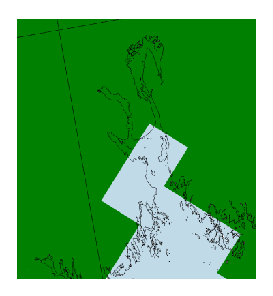
\includegraphics[height=5.2cm]{Oslofjord_A20_grid}}
   \rput[bl](7.5,5.5){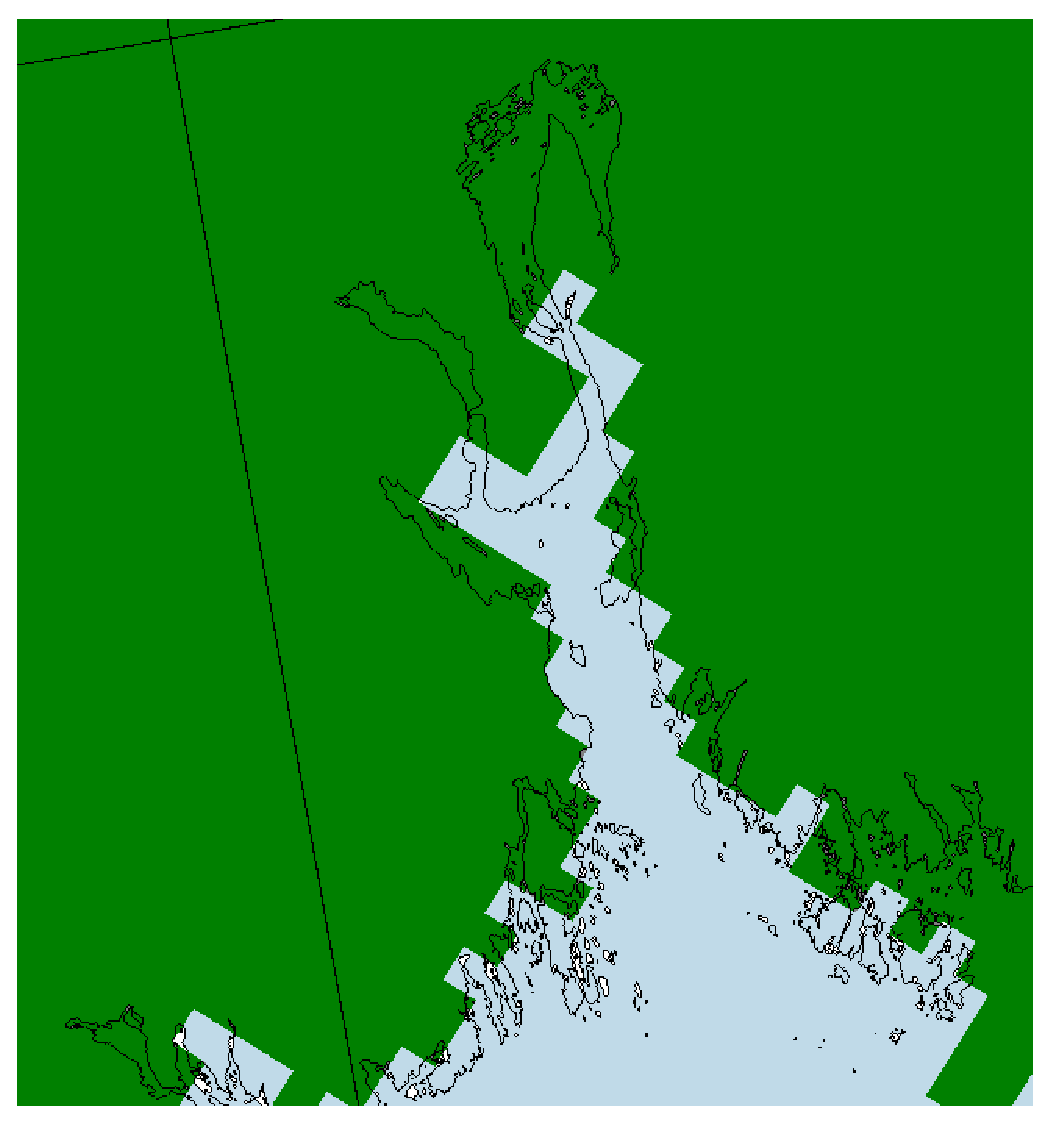
\includegraphics[height=5.2cm]{Oslofjord_N4_grid}}
   \rput[br](7.4,0.0){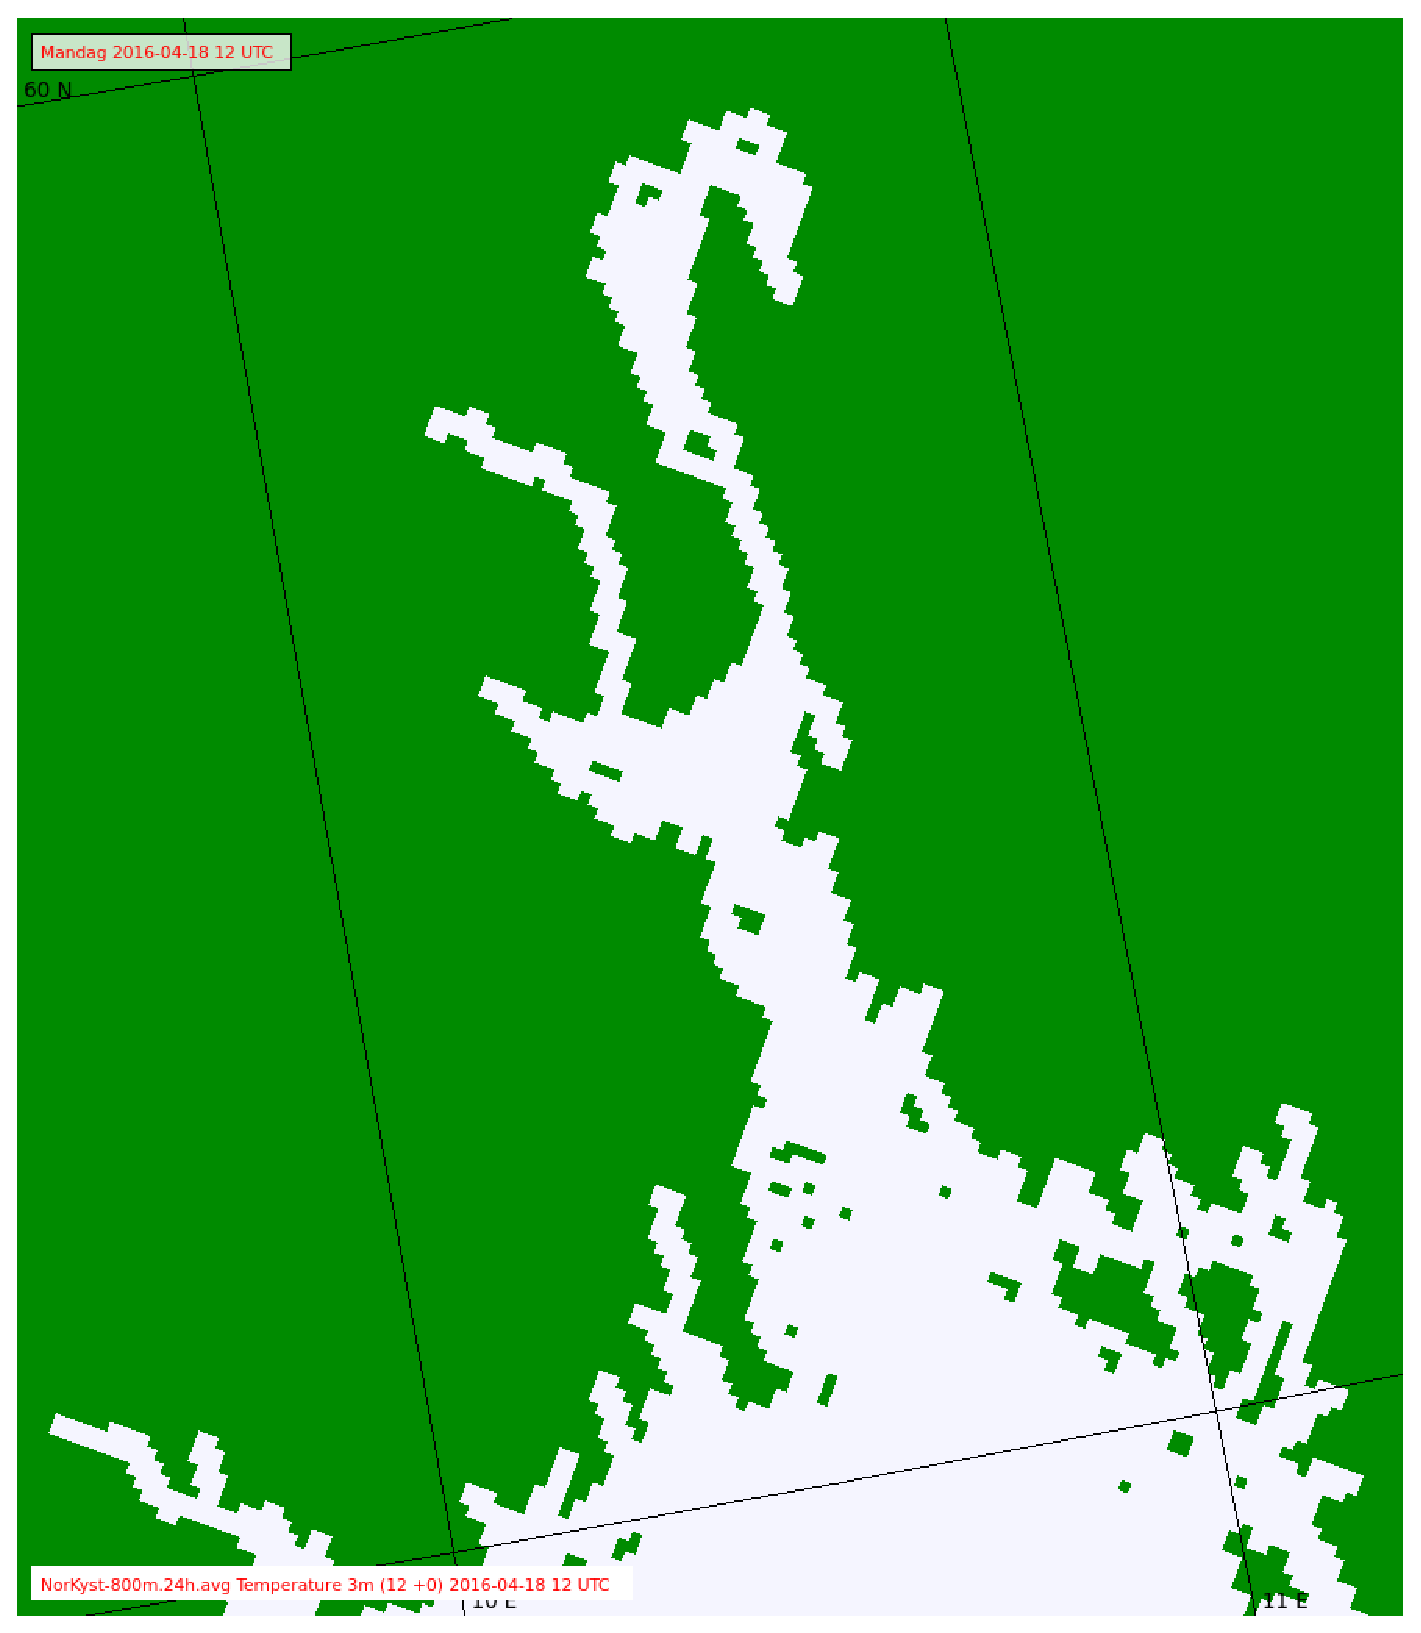
\includegraphics[height=5.2cm]{Oslofjord_N800_grid}}
   \rput[bl](7.5,0.0){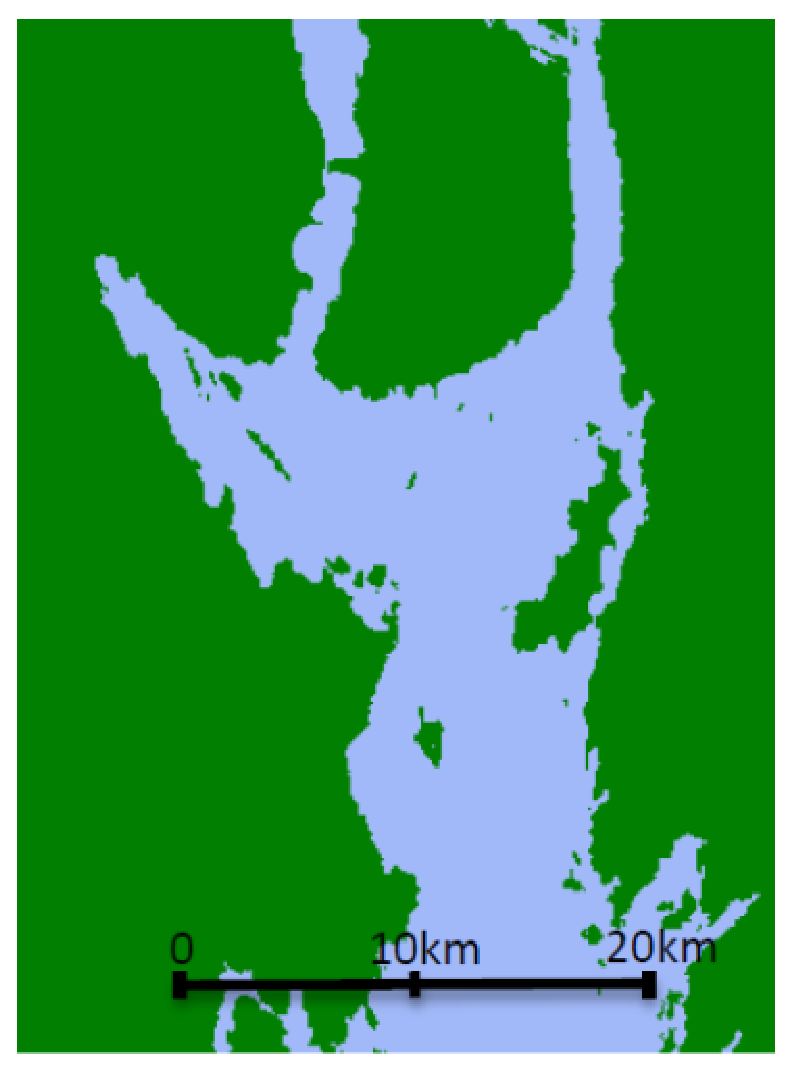
\includegraphics[height=5.2cm]{Midfjord_100m_grid}}
  \end{pspicture}
  \caption{\small Illustrated is the impact of grid resolution on how the Oslofjord is portrayed. Upper two (from left to right) show how the fjord is represented by respectively a 20 km and 4 km grid model, while the two tbottom panels show the same for respectively an 800 m and 100 m grid model zoomed in on Breidangen.} 
  \label{fig:resolution}
 \end{center}
\end{figure}



Despite NorKyst800's relatively high resolution it is still not fine enough to resolve the highly irregular geometry and topography of most Norwegian fjords, and the Oslofjord is no exception. These irregularities consist of small islands, narrow sounds, straits and channels and many smaller scale deep basins and shallow sills as alluded to in Section \ref{subsec:oslofjord} (Figure \ref{fig:map_oslofj}). To properly forecast oil drift, or dispersion of any unwanted substances or contaminants accidentally discharged to the fjord, it is therefore of utmost importance that the underlying fjord model has a realistic representation of the majority of these irregularities. 

The aim of the project FjordOs is therefore to develop an Oslofjord model to resolve most of these features without requiring excessive computer power. We emphasize that such a model, if made operational, will benefit all governmental emergency preparedness models, including those operated by MET Norway. In addition to oil drift these are (i) Search And Rescue or SAR models, which involves forecasting of pathways of floating objects, e.g., man overboard, rafts, small crafts and ships, (ii) transport and spreading of dissolved substances such as nutrients and toxic substances (e.g., nuclear waste), and (iii) growth and drift of toxic algae. Finally we emphasize that resolving the fine scale, submesoscale motion due to the fjord's irregular geometry and topography is required to avoid floating objects, dissolved substances and oil from stranding artificially.  

A vizualization of the impact of resolution on how well the model portrays these irregularities is depicted by Figures \ref{fig:resolution}. As is evident it is only the 100 m grid that represents the Oslofjord as we know it from geographical charts and maps. An example is the small islands in Breidangen (Tofteholmen and M{\o}len simply not present in the 800 m grid model. Likewise the shape and area covered by Bast{\o}y is improved in the 100 m grid, and so is the ridge that cuts into the the Drammensfjord at Svelvik. The same is true regarding topography. An example is displayed by Figure \ref{fig:hvaler2} that compares the topography represented by the new Oslofjord model (FjordOs CL) and Norkyst800. 

To conclude today's forecasting model available for the Oslofjord (NorKyst800) has an insufficient resolution, and a new model of the Oslofjord with a resolution of 100 m or less for most parts of the fjord is needed. The development of a such a model would also greatly benefit all governmental emergency preparedness models including those operated by MET Norway.   
%%%%%%%%%%%%%%%%%%% Figure 2 Bathymetry and currents in the Drøbak area %%%%%%%%%%%%%%%
\begin{figure}[t]
 \begin{center}
  \begin{pspicture}(0,0)(15,8.5)
% Include graphs
   \rput[tl](-0.1,9.5){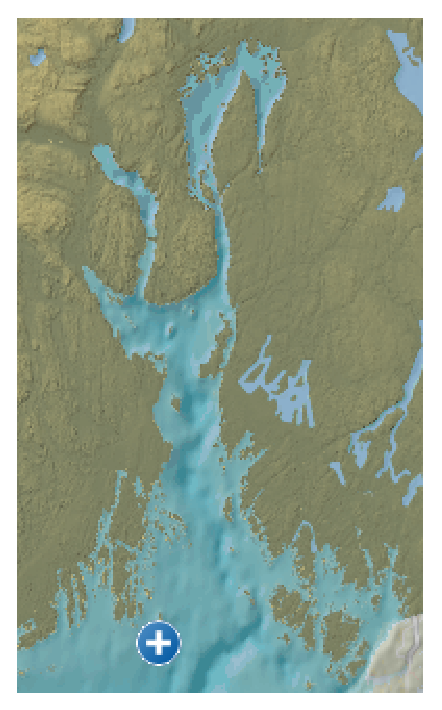
\includegraphics[height=8.5cm]{dyp}}
   \rput[tr](  15,9.5){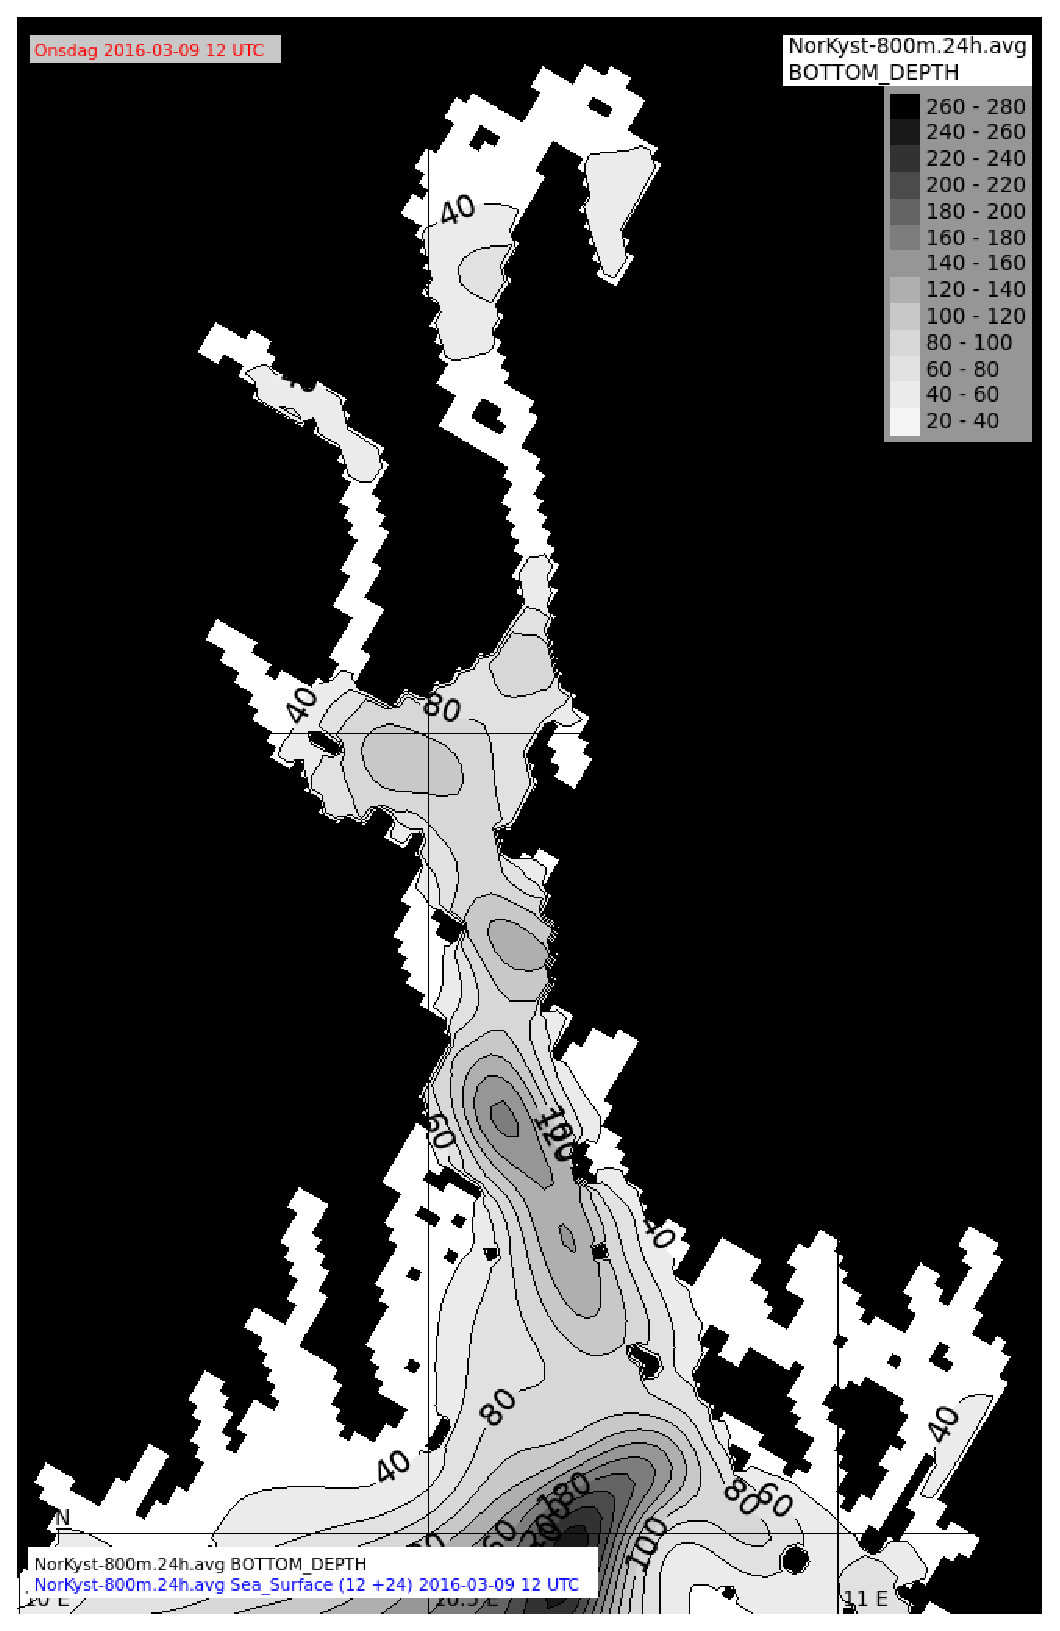
\includegraphics[height=8.0cm]{NorKyst800_topo_oslofjord}}
  \end{pspicture}
  \caption{\small The irregular coastline geometry and topography in the Oslofjord as portrayed in the FjordOs CL model (left) and the NorKyst800 model (right). The color bar (grayscale) indicate depth in meters.}
  \label{fig:hvaler2}
 \end{center}
\end{figure}



% % % % % % % % % % % % % % % % % % % % % % % % % % % % % % % % 
\subsection{Organization of the report}
Notwithstanding that the purpose of this report is to document the technical details regarding the development of the new Oslofjord model FjordOs CL, we have included above some of the characteristics of the Oslofjord (Section \ref{subsec:why}), and provided some of the motivation why a new Oslofjord model is needed (Section \ref{subsec:oslofjord}). Section \ref{sec:model} provides some details on how the curvilinear grid of the FjordOs CL model is constructed. Section \ref{sec:setup} provides some model specifics while Section \ref{sec:forcing} gives details on the model's bathymetry and external forcing such as tides, ocean input through open lateral boundaries, river input as well as atmospheric input. Section \ref{sec:resul} provides some results from an almost two year long hindcast and some test forecasts. Finally we offer a summary and some concluding remarks in Section \ref{sec:summa}. 


\clearpage
\section{The new model}
\label{sec:model}
The FjordOs CL model is based on version 3.6 of the Rutgers Regional Ocean Modeling System (ROMS) adapted to the Oslofjord. ROMS is an open source, numerical ocean model as detailed and documented by \cite{haidv:etal:2008}, \cite{shche:mcwil:2003} and \cite{shche:mcwil:2005, shche:mcwil:2009}. It is freely available and may be downloaded from the ROMS website\footnote{\texttt{http://www.myroms.org/}}. 

In summary ROMS is a free-surface and terrain-following, vertical coordinate ocean model, based on the fully three-dimensional, rotational RANS\footnote{Reynolds Average Navier-Stokes} equations utilizing the hydrostatic and Boussinesq approximations. It is a so called split–explicit model where short time steps are used to advance the surface elevation and barotropic momentum equation, and where a much larger time step is used for temperature, salinity, and baroclinic momentum. In this ROMS employs a two-way time-averaging procedure for the barotropic mode which satisfies the 3D continuity equation. 

% % % % % % % % % % % % % % % % % % % % % % % % % % % % % % % % 
\subsection{Why ROMS?}
An option in ROMS is to use a curvilinear, near orthogonal grid to replace the default orthogonal regular mesh. This option is exploited here. The rationale is that it allows us to minimize the number of, or in reality the area of, ``dry'' grid points. Thereby the number of ``wet'' grid points is maximized without increasing the number of grid points compared to an orthogonal, regular grid mesh model covering the same domain. Thus resolution is increased without increasing the computational burden. In addition it allows us, to a certain extent, to put higher resolution in areas of special interest.
%%%%%%%%%%%%%%%%%%%%%%%%%%%% Figure 6 General curvilinear model %%%%%%%%%%%%%%%%%%%%
\begin{figure}[t]
 \begin{center}
  \begin{pspicture}(0,0)(15,11)
% Include graphs
   \rput[b](7.5,0.0){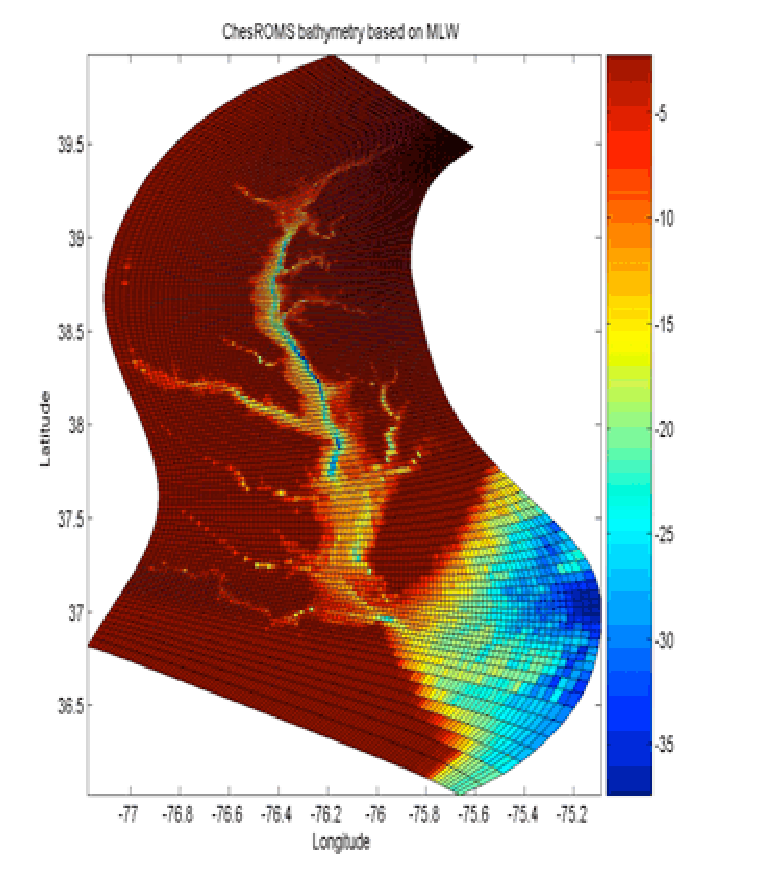
\includegraphics[height=11cm]{ChesROMS_grid}}
  \end{pspicture}
  \caption{\small Examples of a curvilinear grid showing the curvlinear grid used for the Cheasapeake Bay model ChesROMS. Note how the grids follows the land/sea matrix, thus minimizing the number of ``dry'' points. Likewise note how the grid size varies in space.} 
  \label{fig:curvil}
 \end{center}
\end{figure}



The above may also be achieved using unstructured grid models (e.g., FVCOM\footnote{\texttt{http://fvcom.smast.umassd.edu/fvcom/}}, SLIM\footnote{\texttt{http://sites.uclouvain.be/slim/}}). However, the FjordOs research group opted to go for a ROMS development utilizing its curvilinear option rather than starting a completely new strand of model development. The rationale is that 1) ROMS is MET Norway's operational model, 2) MET Norway's scientists are well versed in using ROMS, and 3) MET Norway's scientists have the necessary expertise to operate it. Moreover, none of researchers within the FjordOs participating institutions have any beforehand experience in running and/or setting up a three-dimensional, unstructured model. Nevertheless, to get some insight into the capabilities of an unstructured model, a \emph{two-dimensional version} of FVCOM was used as part of the FjordOs project for the work regarding Moss Harbor \citep{hjelm:etal:2014}.  
%%%%%%%%%%%%%%%%%%%%%%%%%%% Figure 9 FjordOs sketch %%%%%%%%%%%%%%%%%%%%
\begin{figure}[t]
 \begin{center}
  \begin{pspicture}(0,0)(15,10)
   \rput[bl]( 0.0,0.0){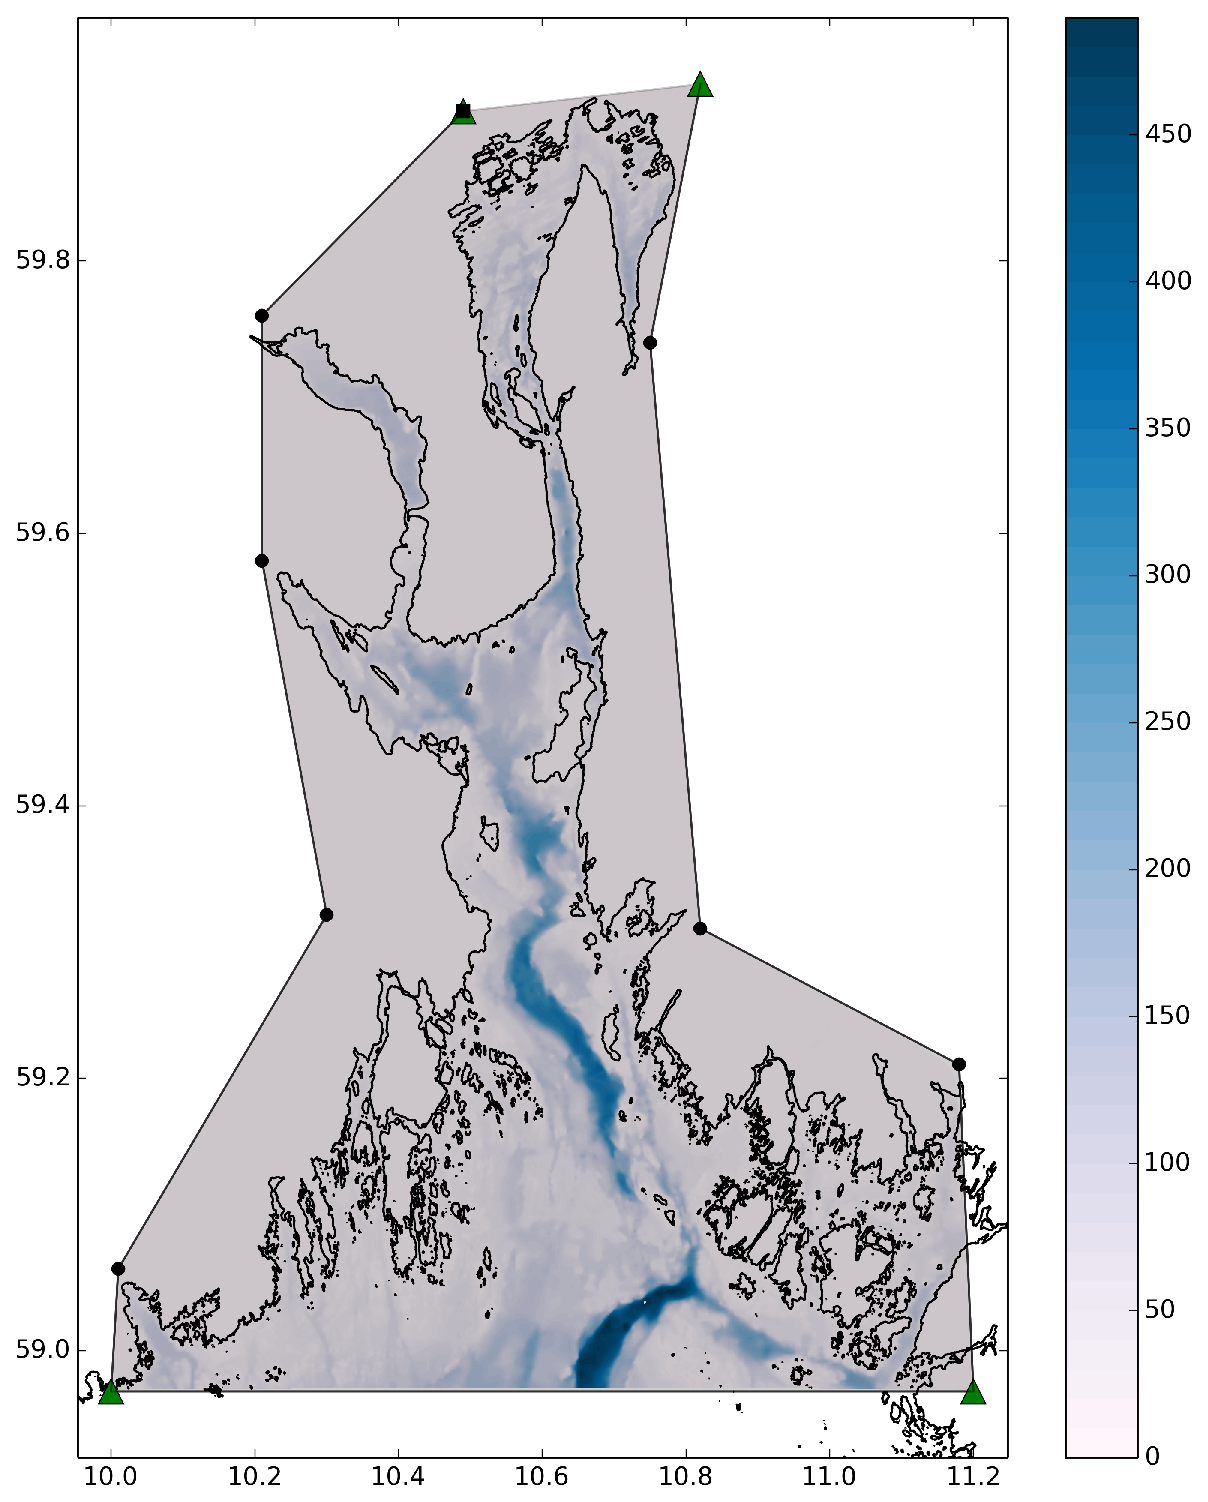
\includegraphics[height=9.0cm]{fig4_crop}}
   \rput[br](15.0,0.0){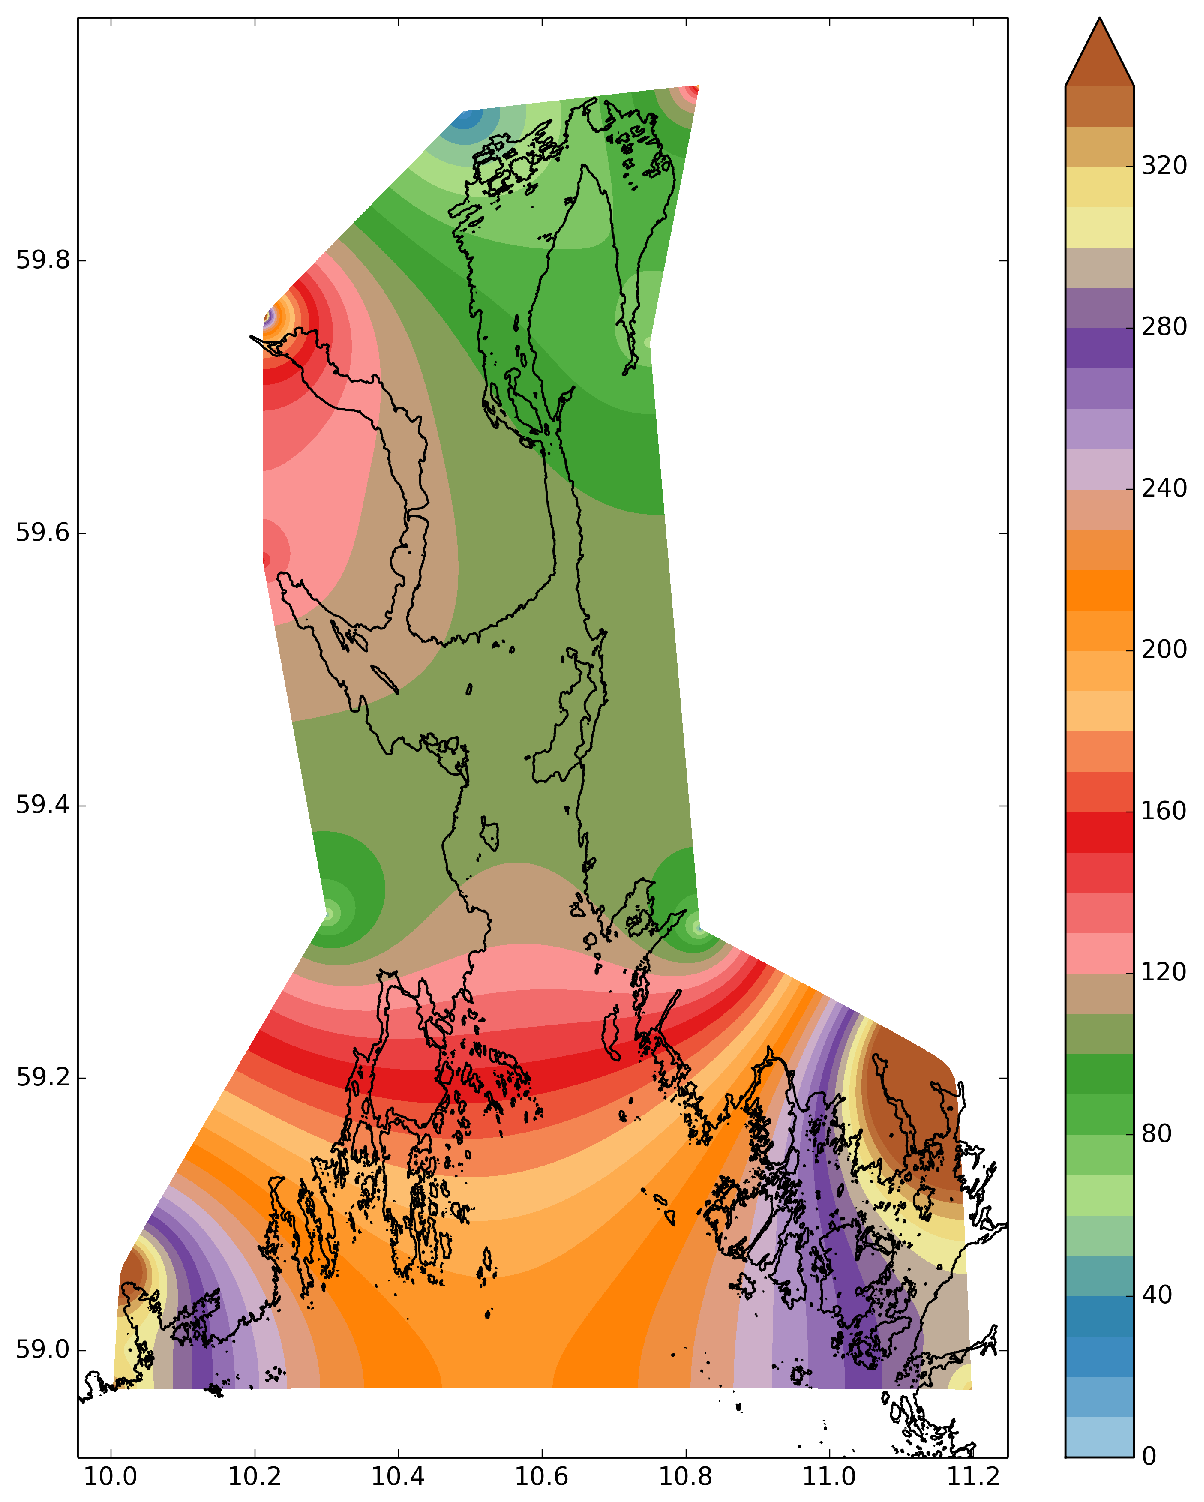
\includegraphics[height=9.0cm]{res_crop}}
   \rput[bl]( 5.0,5.0){\textbf{a)}}
   \rput[br](13.0,5.0){\textbf{b)}}
  \end{pspicture}
  \caption{\small The FjordOs CL computational domain showing (a) the curvilinear grid configuration, and (b) the resulting grid resolution. The right-hand color bar indicates grid size in meters, while the left-hand bluescaled colorbar indicates depth in meters. X-axis is degrees east, and y-axis is degrees north.} 
  \label{fig:fjordos_grid}
 \end{center}
\end{figure}

   

% % % % % % % % % % % % % % % % % % % % % % % % % % % % % % % % 
\subsection{The curvilinear FjordOs CL grid}
Our implementation is inspired in parts by models like the ChesROMS\footnote{\texttt{http://ches.communitymodeling.org/models/ChesROMS/}} model that applied the curvilinear option for an implementation of ROMS for Chesapeake Bay. There exists several different software packages (MATLAB, Fortran, Python, etc.) that can be used for creating curvilinear grids with variable horizontal resolution for ROMS. We use the python-based software package OCTANT\footnote{\texttt{https://github.com/hetland/octant}}. The outer borders of the model domain is defined by corners and nodes as depicted in Figure \ref{fig:fjordos_grid} where corners are depicted as triangles and the nodes as circular dots. There should be a total of exactly four corners to limit the domain. ``Bends'' or nodes in the side walls are then specified so as to follow the land-sea matrix. For this first version of the FjordOs model, we have chosen the corners and nodes using a ``trial-and-error'' approach, so the geometry might be changed in future versions of the FjordOs CL model.
%%%%%%%%%%%%%%%%%%%%%%%%%%% Figure 8 FjordOs ROMS %%%%%%%%%%%%%%%%%%%%
\begin{figure}[t]
 \begin{center}
  \begin{pspicture}(0,0)(15,11)
%  \begin{pspicture}(0,0)(15,18.5)
% Include graphs (the ratio of height to width must be 18.5/8)
% Stående
   \rput[b](7.5,0.0){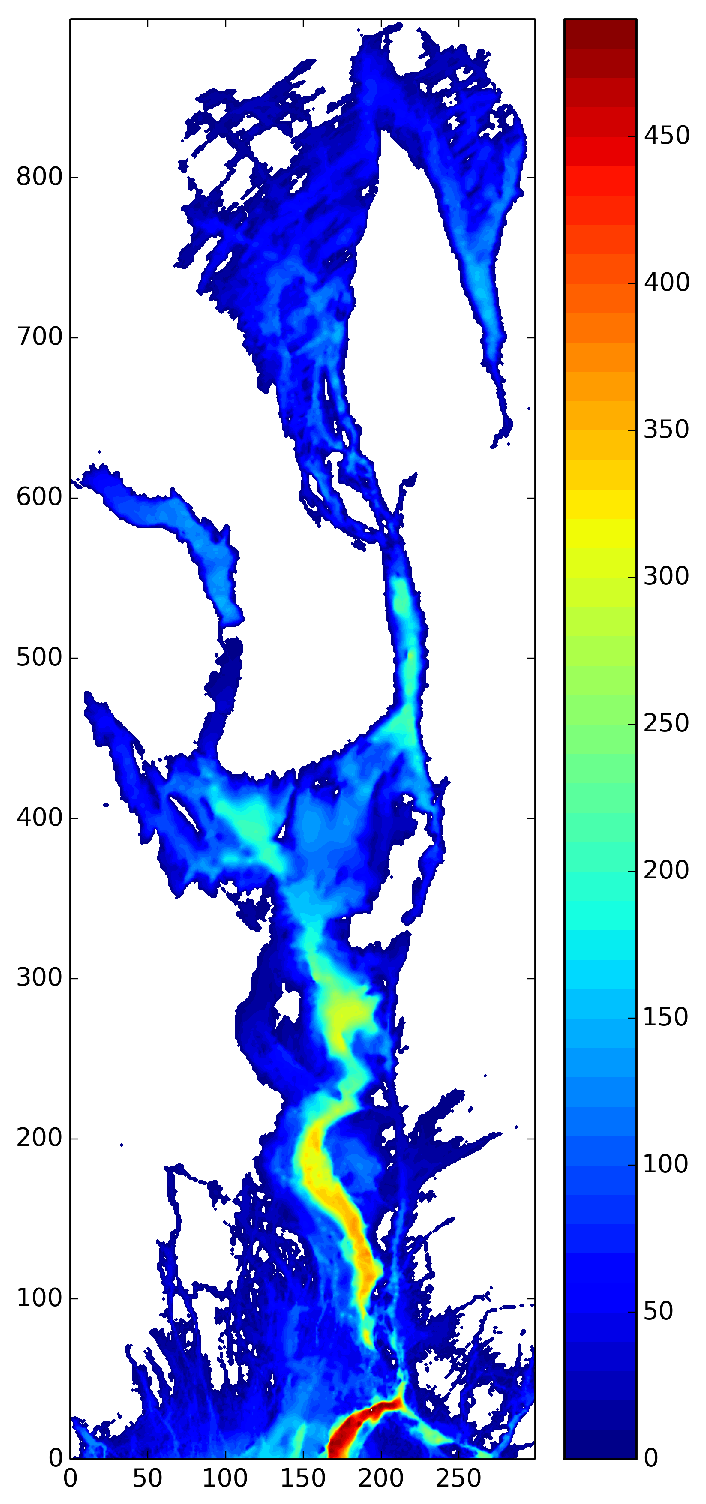
\includegraphics[height=11cm]{fjordos_cl}}
% Liggende
%   \rput[b]( 7.5,0.0){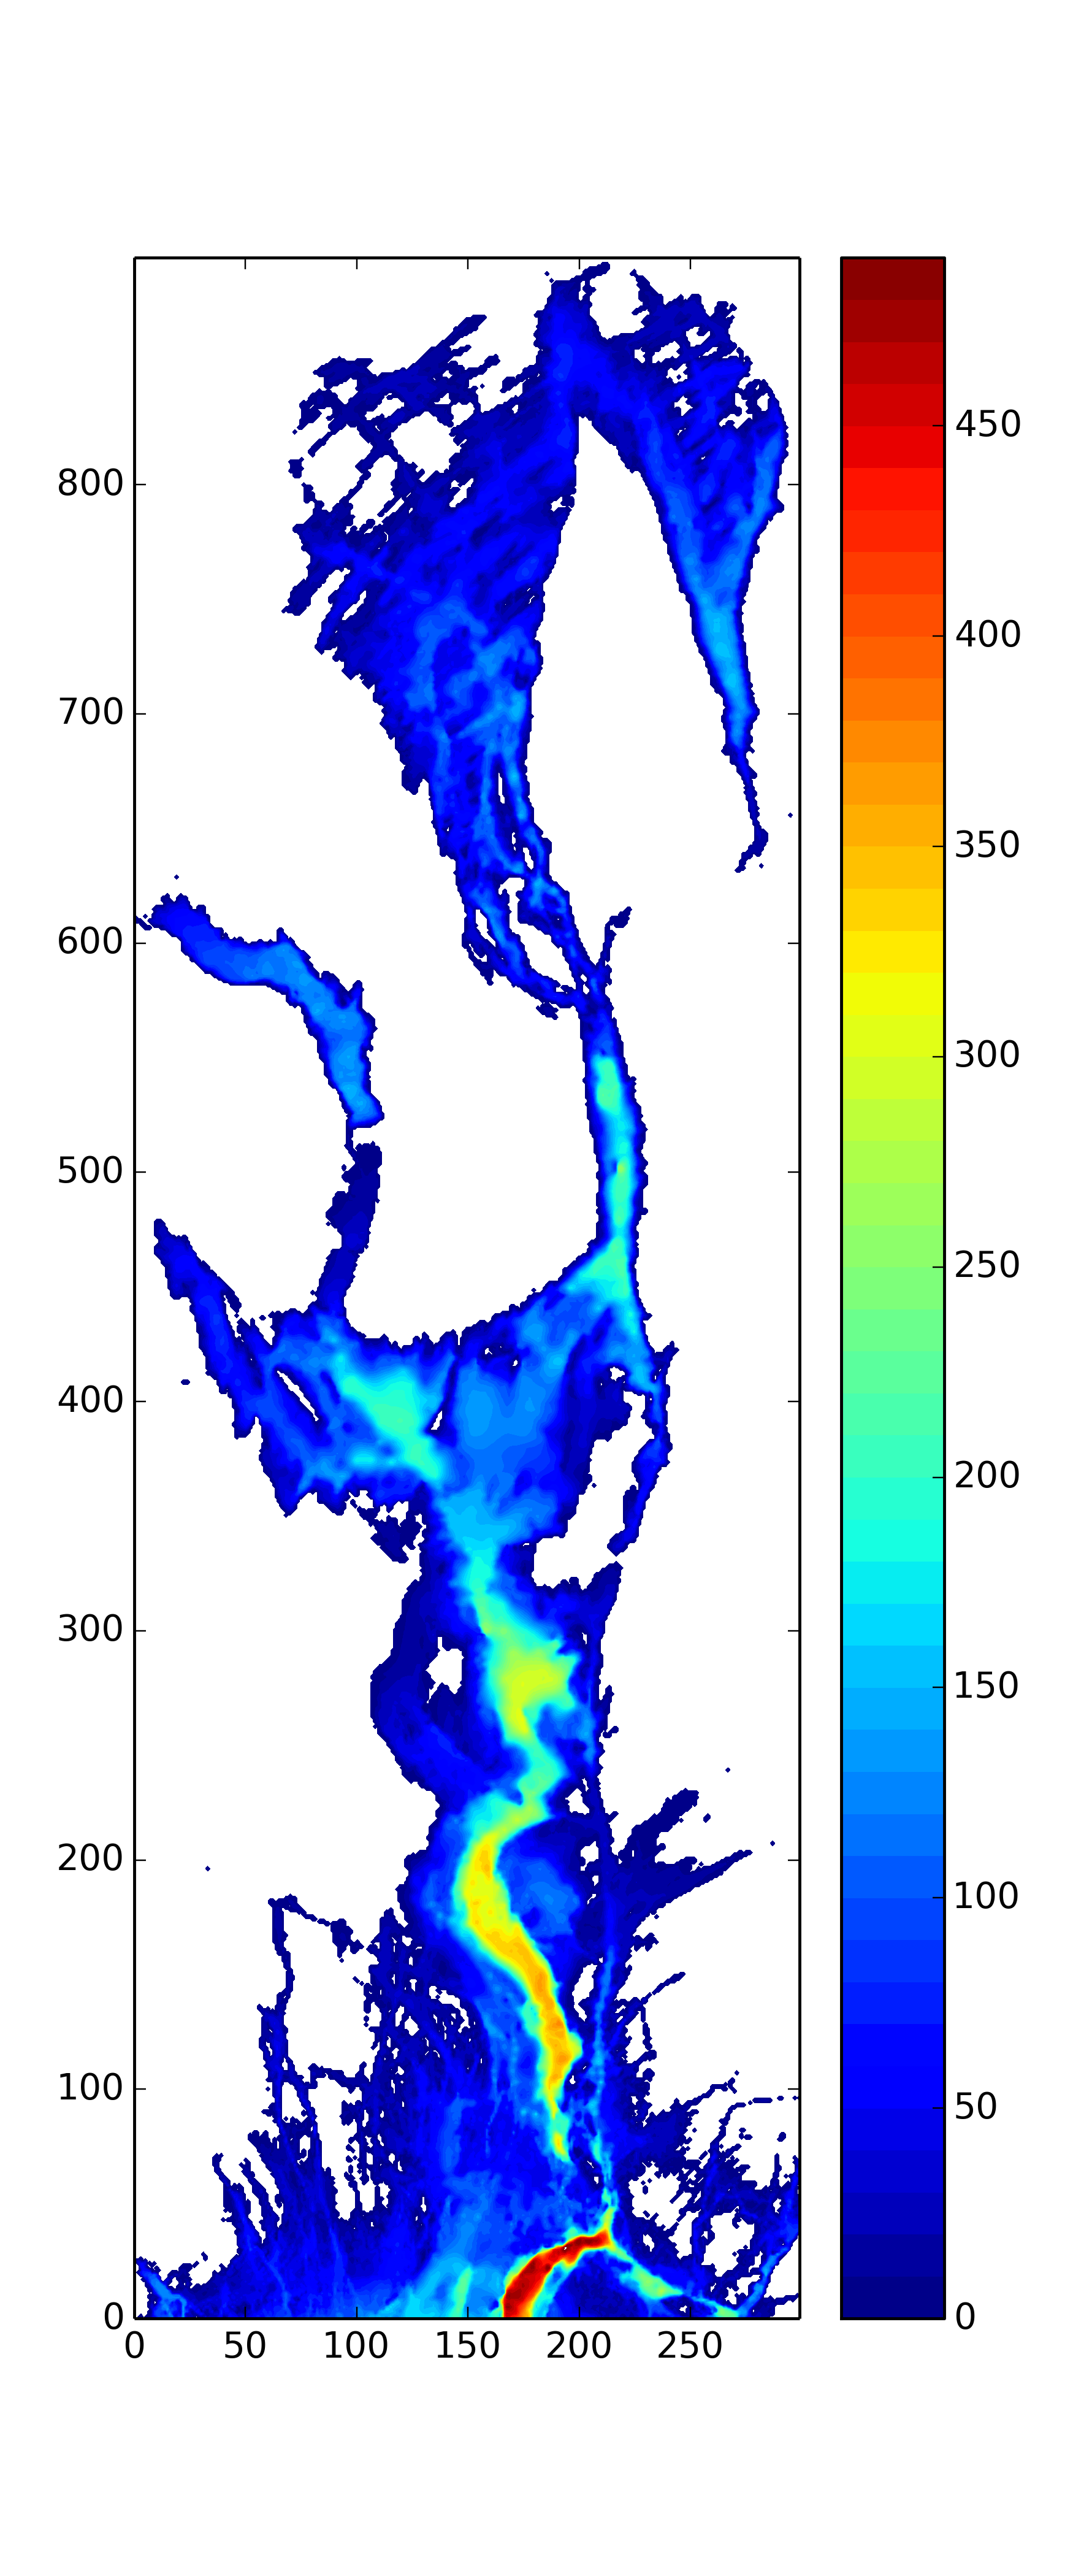
\includegraphics[angle=90,width=15.0cm,height=6.4865cm]{fjordos_roms}}
%   \rput[b]( 7.5,0.0){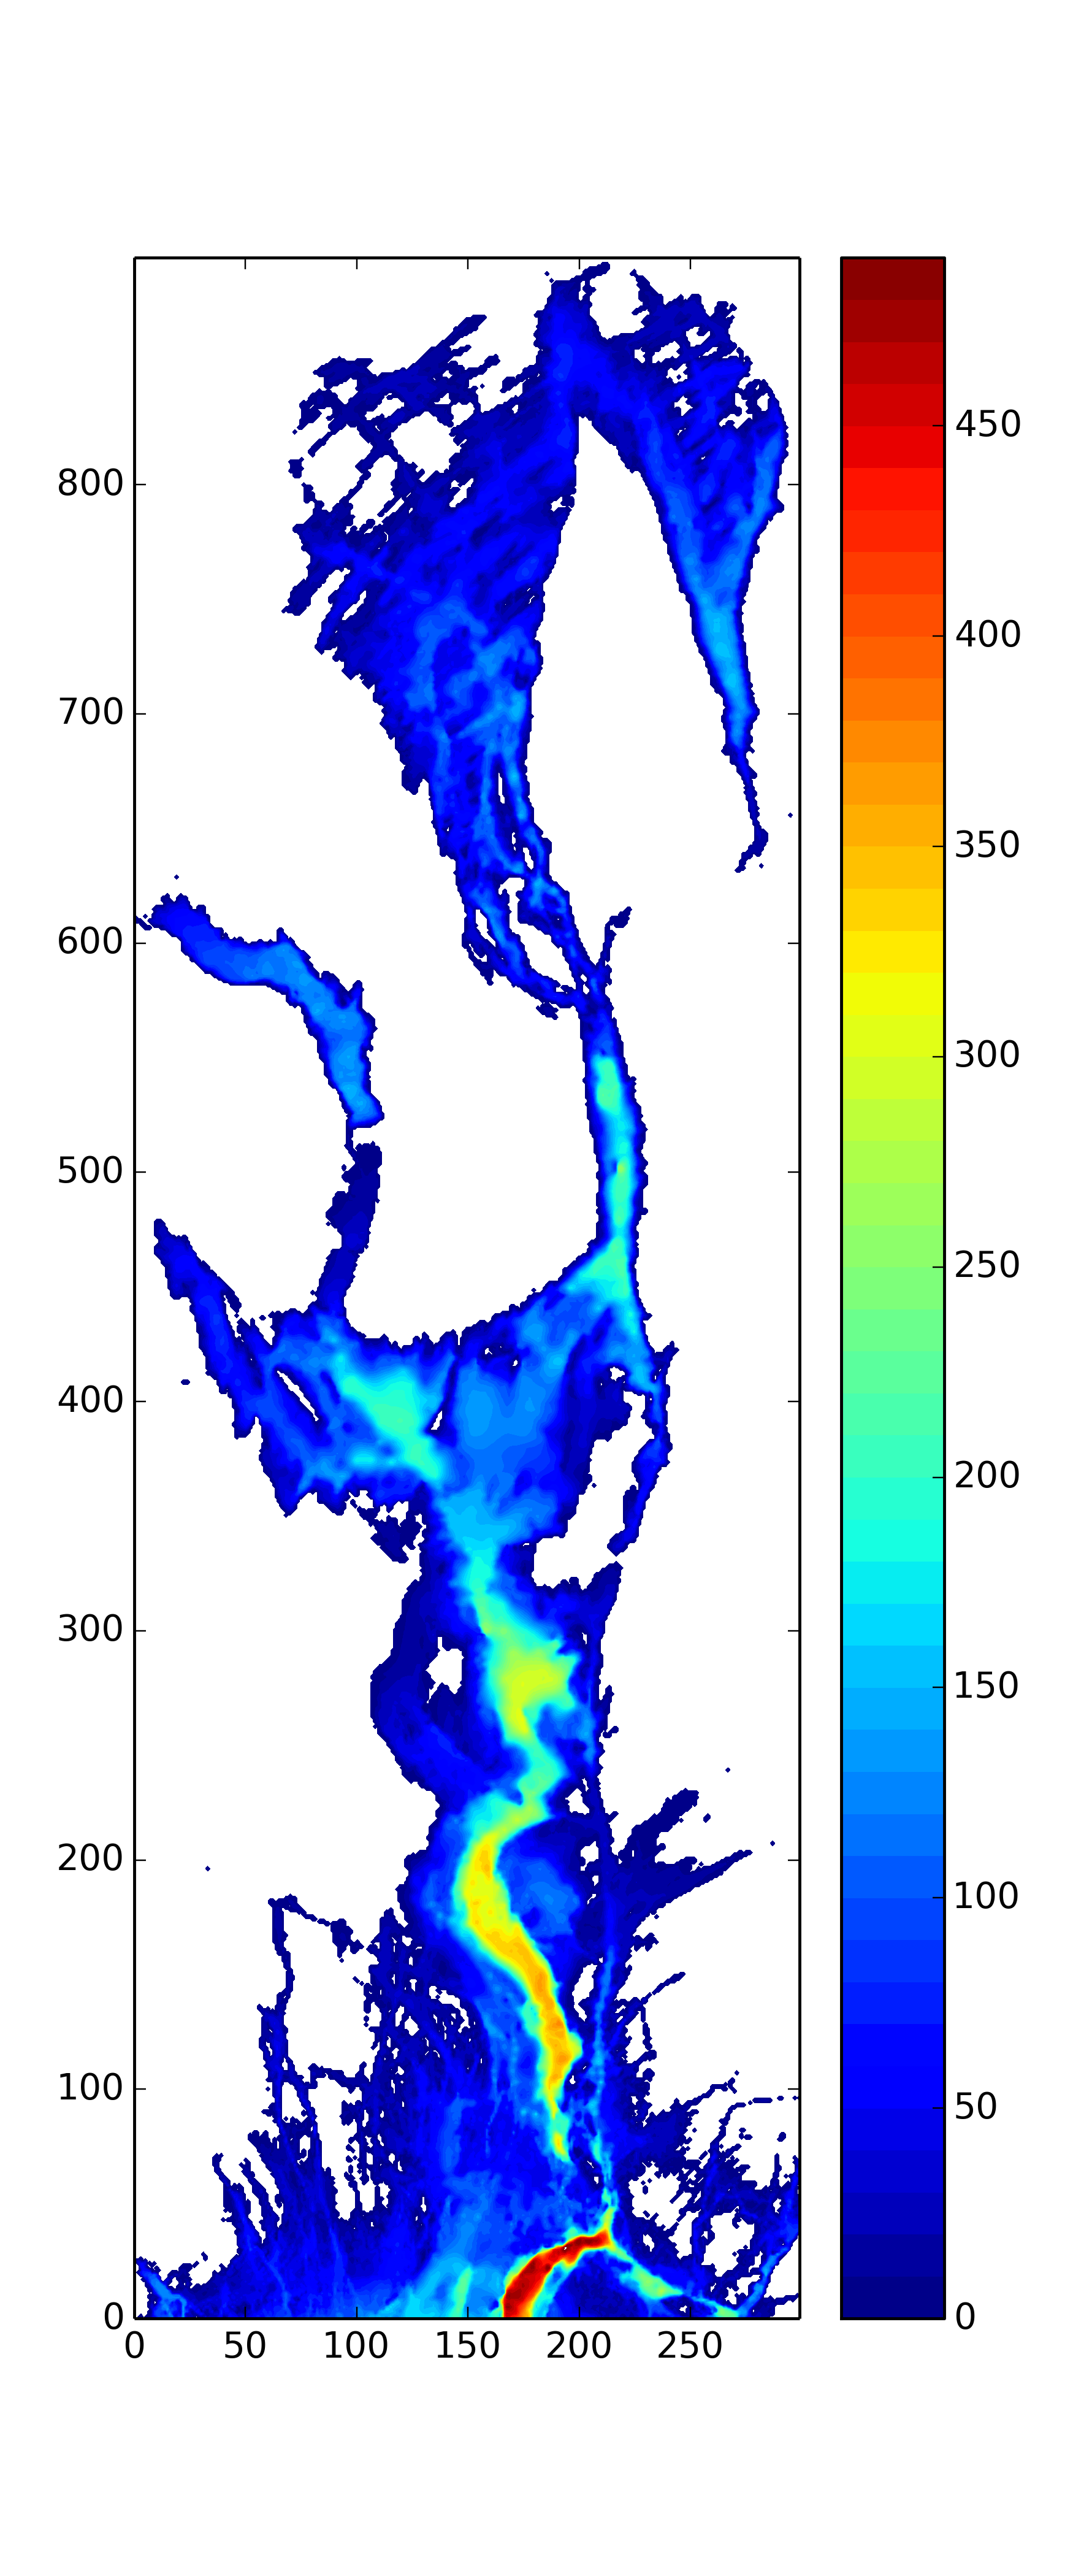
\includegraphics[height=8cm]{fjordos_roms}}
  \end{pspicture}
  \caption{\small The transformed curvilinear grid of the Oslofjord. The colors gives the depth in meters according to the color bar to the right. Model grid numbers associated with the curvilinear grid are given along the axes. There are 300 x 900 grid points.} 
  \label{fig:fjordos_cl}
 \end{center}
\end{figure}



When creating the grid the main constraint is that the grid should be as close to being orthogonal as possible in particular at wet points. One of the advantages of using a package, as for instant the OCTANT package, is that it automatically achieves an optimal orthogonality. To help OCTANT achieving this we have kept the corners and nodes at dry points. The resulting model grid consists of 300 x 900 grid points in the horizontal. As shown by Figure \ref{fig:fjordos_grid} the grid size is less than 200 m in most of the wet areas of the fjord, and less than 100 m in most areas north of Slagentangen (at 59.3N). The exceptions are locations along and close to the southern border where the fjord widens and borders on Skagerrak. Here the grid size of the wet points varies from 200 to 350 m. The increased resolution is perhaps best visualized by Figure \ref{fig:fjordos_cl} displaying the Oslofjord in the curvilinear grid coordinates. Recall that in this coordinate system the grid points are equally spaced. Thus Breidangen and the inner Oslofjord is stretched out in the east-west direction. In reality Breidangen is about one third of the geographical distance across the southern open boundary. Thus the resolution in Breidangen and the inner Oslofjord is in effect increased with a factor of three. In the {\DR} sound the east-west grid size in the curvilinear grid is about 80 m.  




\section{Model specifics}
\label{sec:setup}
The version of ROMS we use is downloaded from the main ROMS repository\footnote{\texttt{http://www.myroms.org/svn/src/tags/roms-3.6/}}, and includes the 3.6 version of the code from Hernan Arango (the Rutgers branch). This version is without sea ice, but in contrast to most other ROMS versions allows data assimilation.

ROMS consists of several built-in schemes and algorithms, and it uses C-preprocessing to activate the various physical and numerical options. ROMS is a very up-to-date and modular code written in F90/F95. The entire input and output data structure of the model is via NetCDF which facilitates the interchange of data between computers, user community, and other independent analysis software.

In the horizontal the model state variables are staggered using an Arakawa C-grid as shown by Figure \ref{fig:romsgridh}. The free-surface, density, and active/passive tracers are located at the center of the cell ($\rho$ points) whereas the horizontal current components ($u$, $v$) are located at the west/east and south/north edges of the cell, respectively. In ROMS all the arrays containing state variables are dimensioned with the same size in the horizontal to facilitate parallelization. The size of the model's horizontal grid is defined in the ROMS input file (\texttt{ocean.in}) with interior points only (denoted $L-1$ and $M-1$ in Figure \ref{fig:romsgridh}). However, all input forcing files must, and output result files do, contain fields at the full grid, which includes the one extra grid point in the boundary zone.
%%%%%%%%%%%%%%%%%%% Figure 2 Bathymetry and currents in the Drøbak area %%%%%%%%%%%%%%%
\begin{figure}[t]
  \begin{pspicture}(0,0)(15.5,10)
% Include graphs
   \rput[b](6.5,0){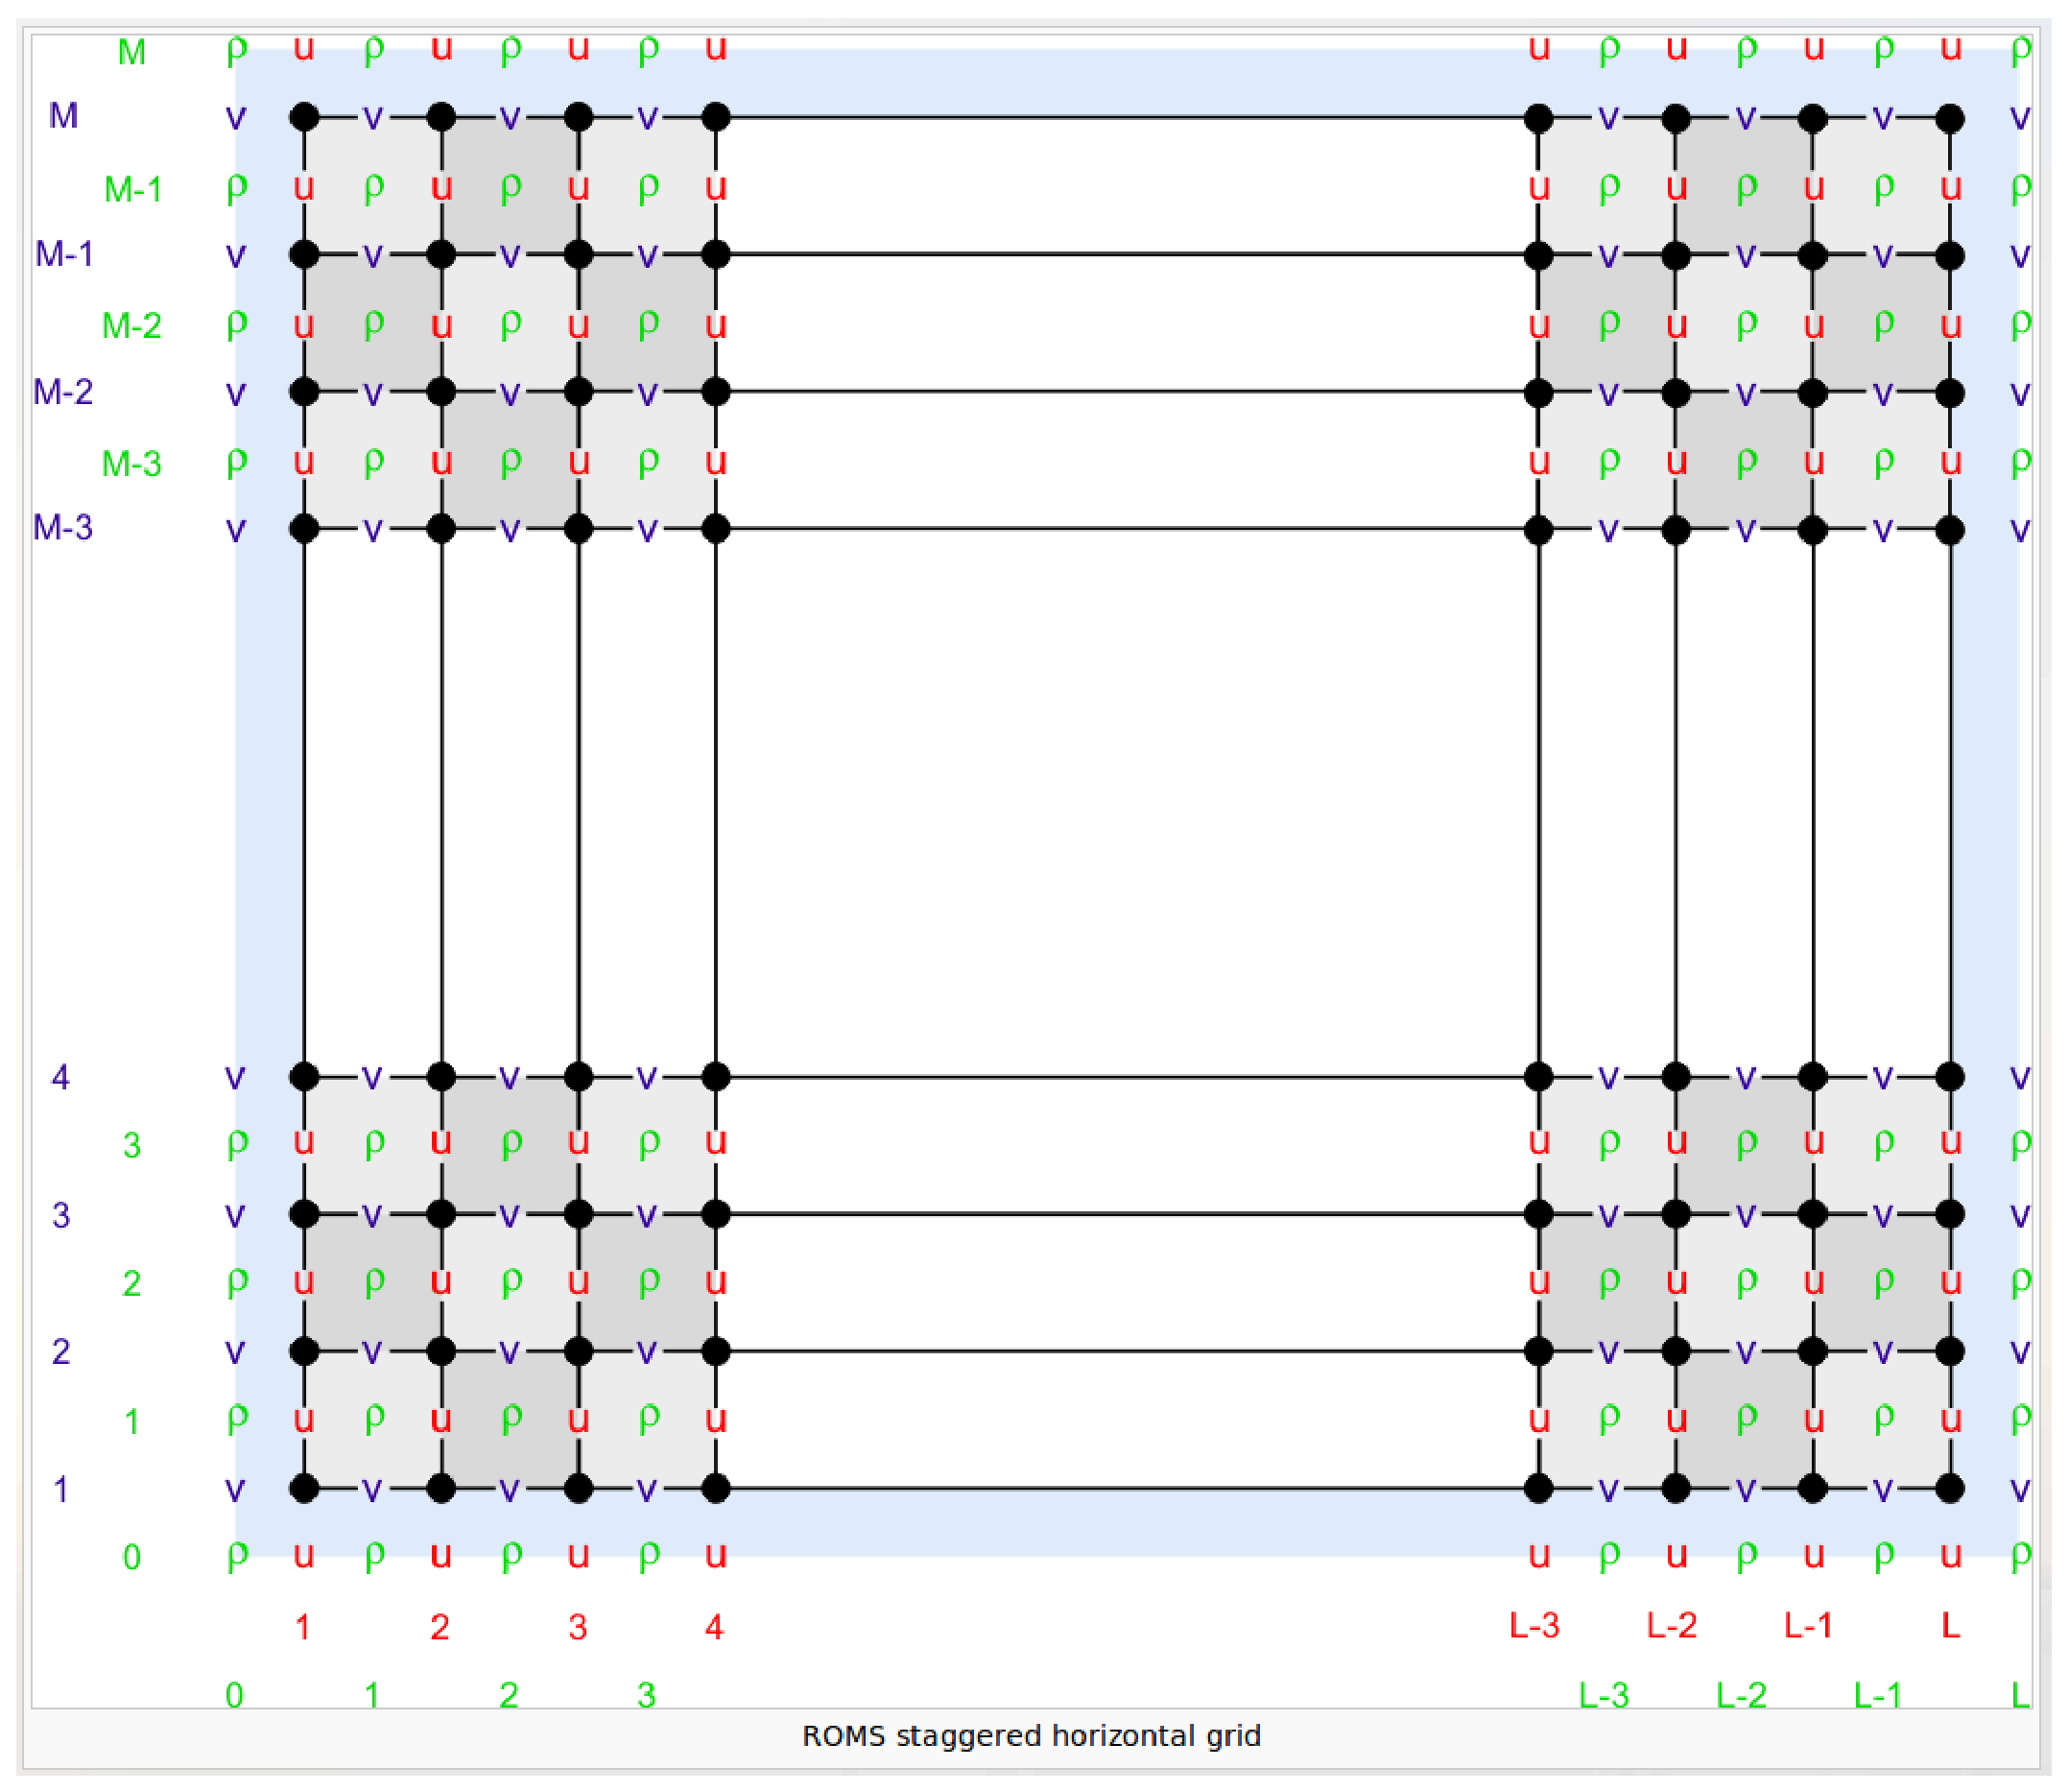
\includegraphics[height=10cm]{ROMS_staggered_horizontal_grid}}
   \rput[rt](15.5,10){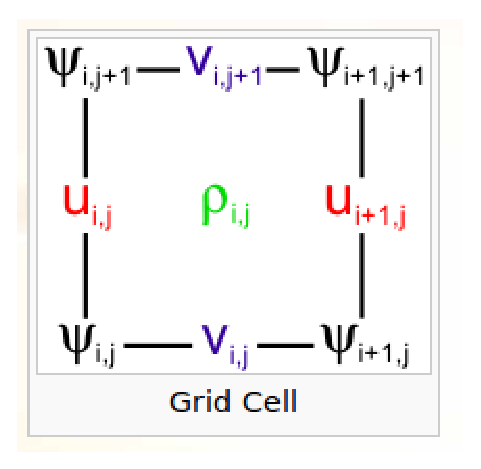
\includegraphics[height=3cm]{ROMS_grid_cell_numbering}}
  \end{pspicture}
  \caption{\small The horizontal distribution and numbering system of variables in the ROMS grid. The figure is downloaded from the \texttt{http:www.myroms.org} website.}
  \label{fig:romsgridh}
\end{figure}



In the vertical ROMS make use of a stretched terrain-following coordinate denoted $s=s(x,y,z,t)$, sometimes referred to as modified $\sigma$-coordinates \citep{song:haidv:1994}. As a result, each grid cell has a different level thickness (denoted $H_z = \pzs z$) and volume. The model state variables are vertically staggered so that horizontal momentum, density, and active/passive tracers are located at the center of the grid cell. The vertical velocity and vertical mixing variables ($Akt$, $Akv$, etc) are located at the bottom and top faces of the cell as displayed by Figure \ref{fig:romsgridv}. The stretched coordinate allows increased resolution in areas of interest, such as thermocline and bottom boundary layers. 
%%%%%%%%%%%%%%%%%%% Figure 2 Bathymetry and currents in the Drøbak area %%%%%%%%%%%%%%%
\begin{figure}[t]
  \begin{pspicture}(0,0)(15,10)
% Include graphs
   \rput[b](7.5,0){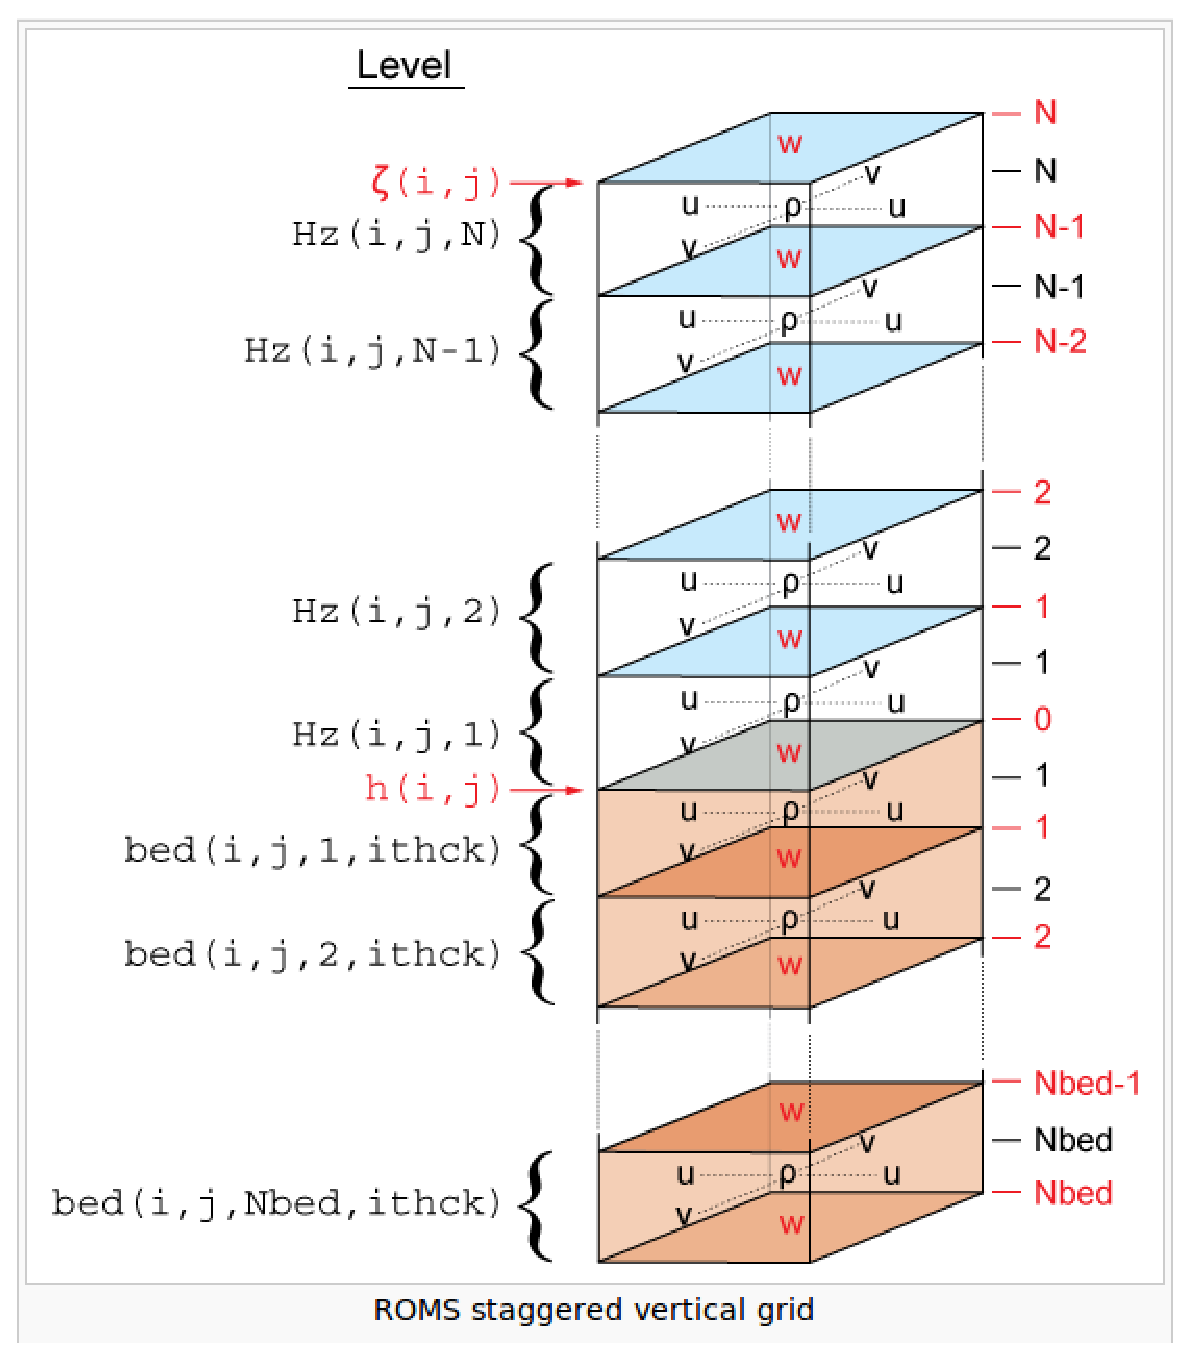
\includegraphics[height=10cm]{ROMS_staggered_vertical_grid}}
  \end{pspicture}
  \caption{\small The vertical distribution and numbering system of variables in the ROMS grid. The figure is downloaded from the \texttt{http:www.myroms.org} website.}
  \label{fig:romsgridv}
\end{figure}



Regarding the FjordOs CL model we opted for 42 $s$-layers with an increased resolution in the surface layer and a reduced resolution near the bottom. This was achieved by letting $Vtransform=2$, $Vstretching=4$, $h_c = 50$ m, $\th_s = 3.0$ and $\th_b = 0.5$, where $h_c$ is a critical depth above which the vertical spacing of the $s$-levels become nearly uniform and independent of the local depth $h$ as long as $h >> h_c$. The minimum depth was set to $h_{min}=2$ m. By having the $s$-levels more confined to the surface layers less smoothing is necessary to minimize the pressure gradient error inherent in all terrain-following coordinate models \citep{haney:1991}. The smoothing is controlled by two parameters referred to as the $r$-factors (see Section \ref{subsec:bathy}). An example of the vertical distribution of the $s$-levels is shown by Figure \ref{fig:roms_slevels}.
%%%%%%%%%%%%%%%%%%% Figure 2 Bathymetry and currents in the Drøbak area %%%%%%%%%%%%%%%
\begin{figure}[t]
  \begin{pspicture}(0,0)(15,10)
% Include graphs
   \rput[b](7.5,0){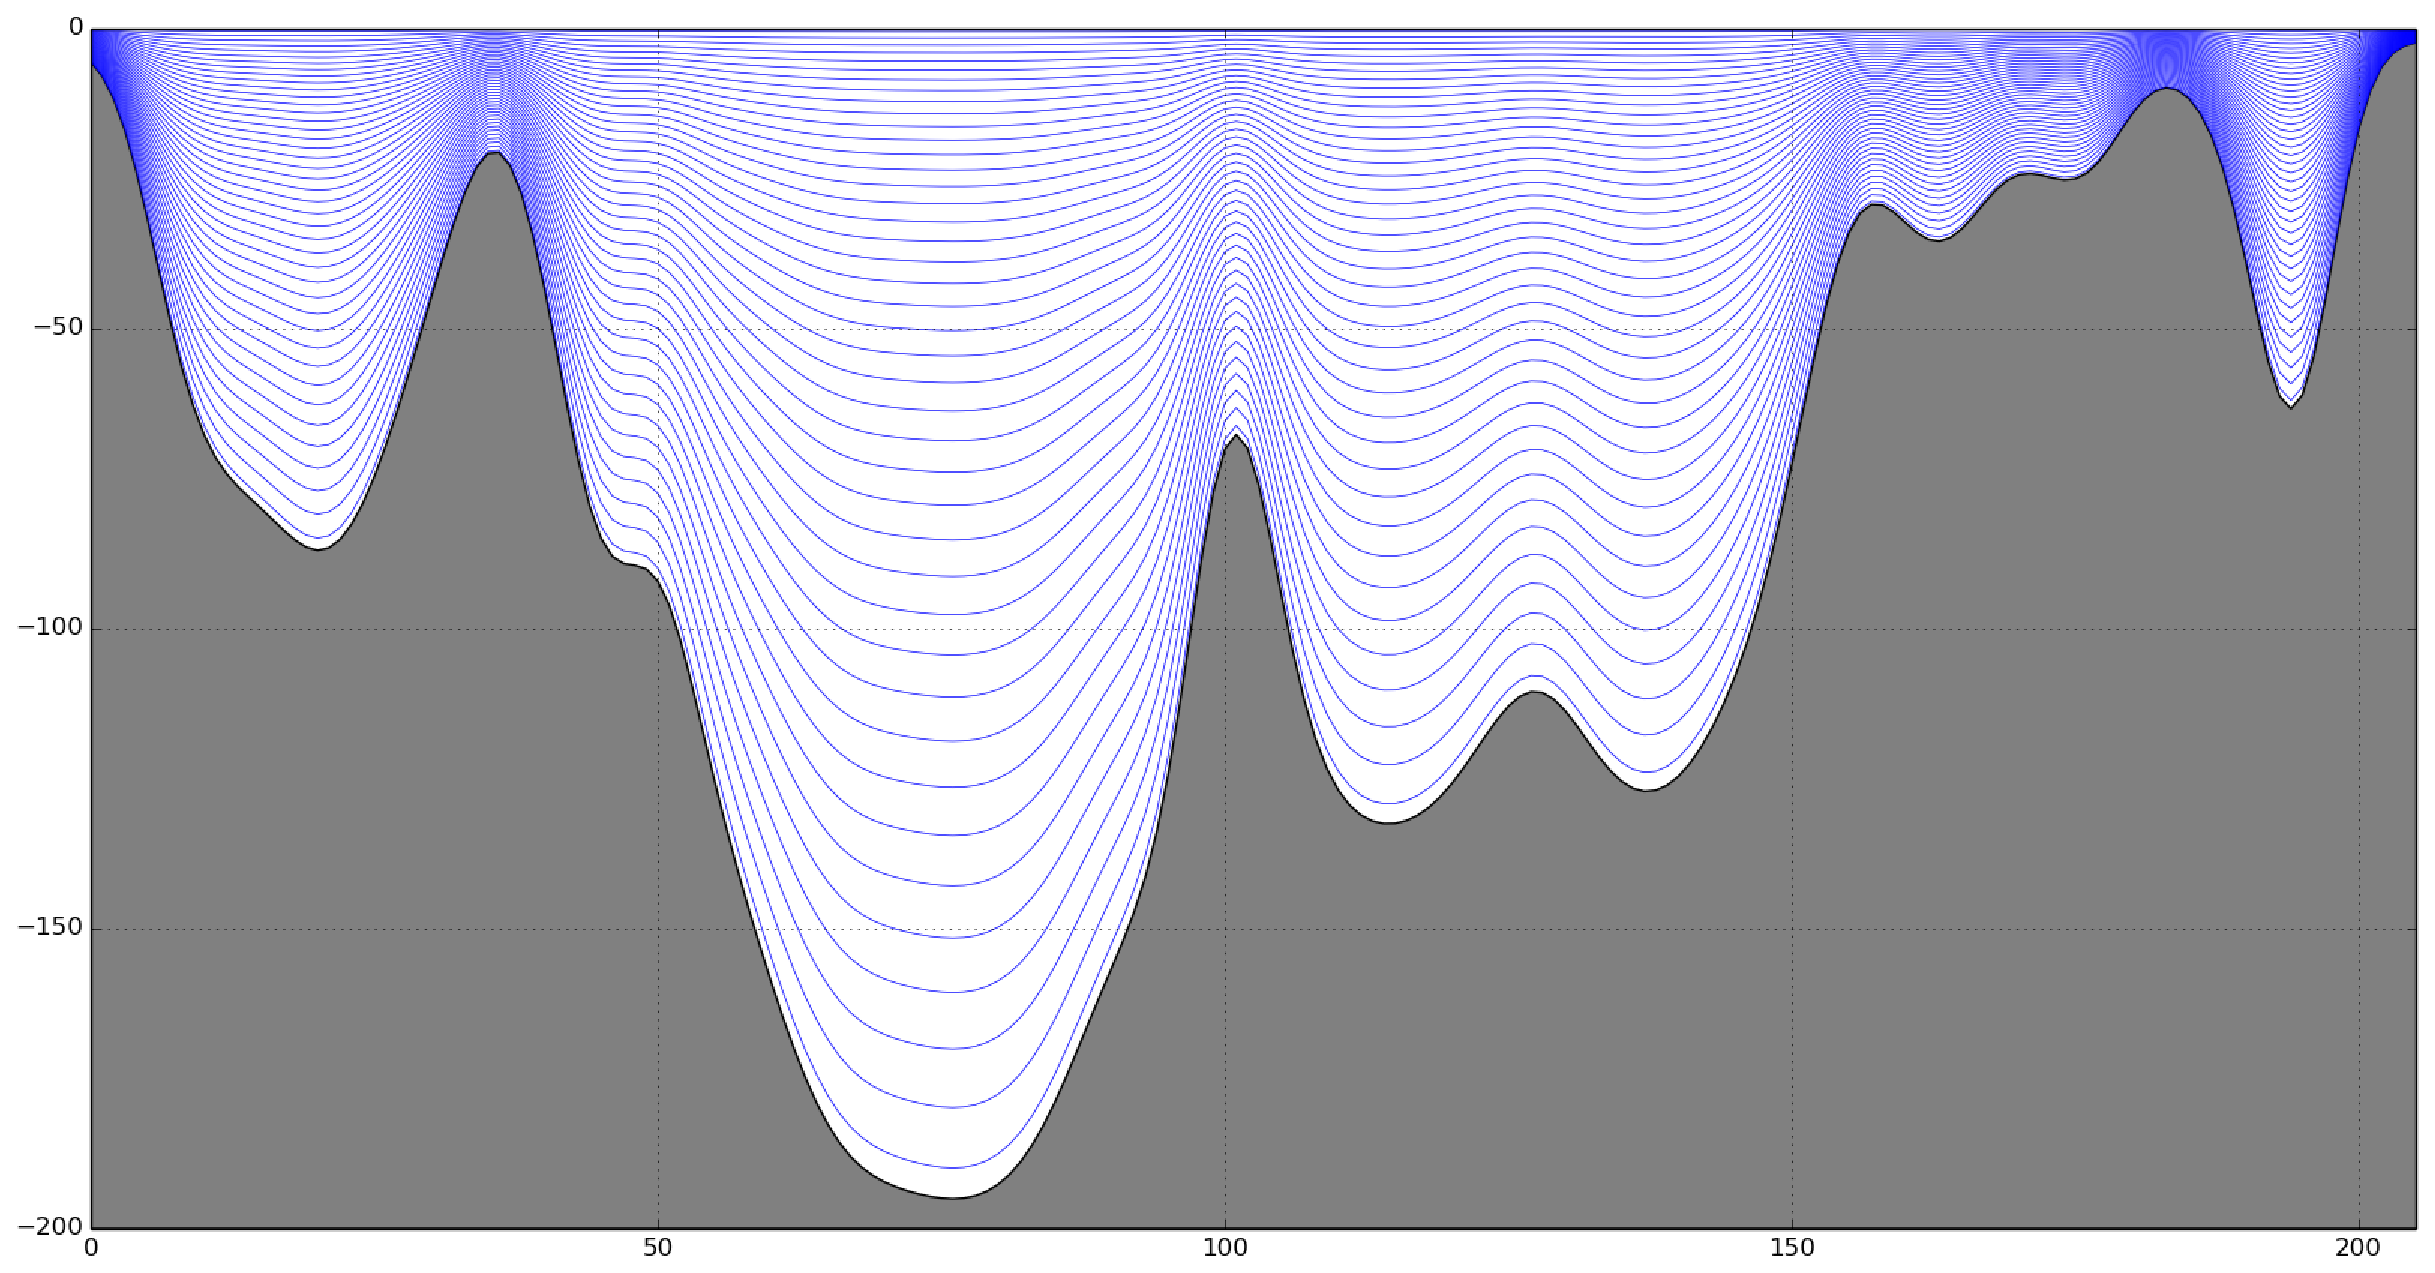
\includegraphics[height=5cm]{fjordos_vertical_coordinates}}
  \end{pspicture}
  \caption{\small Sketch of the vertical distribution of $s$-levels in the FjordOs model (cross-section at Breiangen, y=600).}
  \label{fig:roms_slevels}
\end{figure}



ROMS has several options that determines the numerical schemes for lateral advection of momentum and tracers. In the results displayed in Section \ref{sec:resul}, we have employed a fourth-order, centered advection scheme. This necessitate the application of explicit lateral eddy viscosity and diffusion. To parametrize the subgrid-scale vertical mixing processes we use the Generic Length Scale (GLS) scheme  \citep{umlau:burch:2003}. Values chosen for the various parameters and options activated to derive the results exhibited by Section \ref{sec:resul} are listed in Table \ref{tab:parameters}. 
\begin{table}[h]
 \begin{center}
  \caption{List of FjordOs CL model set-up parameters.}
   \begin{tabular}{lccl}
   \hline
    Parameter				& Symbol	& Value	& Unit		\\
   \hline
    Vtransform				& -		& 2 	& -		\\
    Vstretching 			& -		& 4	& -		\\
    Number of layers			& $k$ 		& 42 \\
    %Explicit lateral eddy viscosity	& $A_M$		& 	& m$^2$s$^{-2}$	\\
    Critical depth			& $h_c$		& 50	& m		\\
    Surface resolution factor		& $\th_s$	& 3.0	& -		\\
    Bottom resolution factor		& $\th_b$	& 0.5	& -		\\
    %.. 					& ..		& ..	&		\\
   \hline
   \end{tabular}
  \label{tab:parameters}
 \end{center}
\end{table} 



To run the model several external inputs or forcing have to be supplied, such as atmospheric input, river input, tides, and input of sea level, currents and hydrography at the model's open lateral boundaries, in addition to bathymetry as described in Section \ref{sec:forcing}.   

%%%%%%%%%%%%%%%%%%%%%%%%%%%%%%%%%%%%%%%%%%%%%%%%%%%%%%%%%%%%%%
\clearpage
\section{Bathymetry and external forcing}
\label{sec:forcing}
% % % % % % % % % % % % % % % % % % % % % % % % % % % % % % % % 
\subsection{Bathymetry}
\label{subsec:bathy}
The bathymetry data for the FjordOs CL model is supplied by NIVA. The original resolution was 25 m. Modifications of some of the topographical features were needed to fulfill the restriction of avoiding one-point bays in ROMS. Additionally, effort was made in opening up narrow straits important for the local circulation, in particular advection of brackish water originating from rivers. To avoid model instability and/or spurious deep currents the final masked bathymetry is smoothed to fulfill a requirement on the ROMS slope or $r_{x0}$-factor \citep{beckm:haidv:1993}, defined as
\be
 r_{x0} = \frac{ h_{i-1} - h_{i} }{ h_{i-1} + h_{i} }
\ee
where $h$ is the bottom depth and the index $i$ indicates a model grid point. The final bathymetry in FjordOs CL has a maximum $r_{x0} = 2.372424E-01$.

In addition, Haney (1991) argues that in order for difference schemes to be hydrostatically
consistent, the parameter settings must be defined so that
\be
\label{eq:haney}
 \left| \frac{s}{h} \px h\right|\frac{\Dx}{\Ds} < 1
\ee
where $s$ denotes the value of the terrain-following $s$-layer (0 at the surface, -1 at the bottom), $\px h$ is the difference in depth over a grid cell, $\Dx$ is the grid size and $\Ds$ is the vertical distance between $s$-layers. For instance in a grid cell with total depth of $h_i=1000$ m, with a neighboring depth of $h_i-1=900$ m, with a grid resolution $\Dx=800$ m, near the seabed between $s$-layer 0.9 and 1.0, the Haney number would be 1. In practice the Haney number is estimated by
\be
 r_{x1} = r_{x0}\frac{Z_w(i,j,k) - Z_w(i-1,j,k) + Z_w(i,j,k-1) - Z_w(i-1,j,k-1)}
                     {Z_w(i,j,k) + Z_w(i-1,j,k) - Z_w(i,j,k-1) + Z_w(i-1,j,k-1)}
\ee
where $Z_w$ is the depth of the water column at grid coordinates ($i,j$) and at $s$ level $k$. In the case where the second deepest $s$-level of grid cell ($i,j$) has equal depth to the deepest level in grid cell ($i-1,j$) the Haney number will be 1. Obeying the criteria (\ref{eq:haney}) ensures that for a certain grid size the vertical grid increment is small enough for the $s$-layer immediately above (below) remains above (below) within the distance of one grid interval. Although there is no mathematically well-defined thresholds a rule of thumb is $r_{x1} \lesssim 10$. There is no consensus in the ROMS community on the upper limit for $r_{x1}$ though. Thus one has to consider the recommendations on thresholds to be the outcome of practical experience. For instance Kate Hedstr{\o}m allows a Haney number of several tens while Alexander Shchepetkin considers a value below 3 as ``safe and conservative'' and values above 8-10 as ``insane''\footnote{ROMS Discussion Forum (\texttt{https://www.myroms.org/forum/viewtopic.php?f=14\&t=612)}}. It boils down to controlling the pressure gradient error. FjordOs CL has a maximum $r_{x1} = 1.424997E+01$. %%%Recent examples for Norwegian waters and fjords are \cite{albre:etal:2011} and \cite{staal:roed:2016}. The latter applied ROMS for the inner part of the Oslofjord inside of the {\DR} sill. %NMK: skjønner ikke hvordan dette hører hjemme her...

% % % % % % % % % % % % % % % % % % % % % % % % % % % % % % % % 
\subsection{Atmospheric forcing}
\label{subsec:atmos}
The necessary atmospheric input is extracted from the AROME-MetCoOp model that runs operationally at MET Norway \citep{mulle:etal:2015}. It is a convective scale (non-hydrostatic) model providing forecasts with a lead time of 66 hours four times a day from analyses at 00, 06, 12 and 18 UTC. It has a grid resolution of 2.5 km, and was made operational in March 2014. Available to us are analyses and forecasts saved every six hours since April 2014, as well as real time forecasts covering the are shown in Figure \ref{fig:arome}.
%%%%%%%%%%%%%%%%%%%%%%%%%%% Figure 3 Godafoss %%%%%%%%%%%%%%%%%%%%%%%%%%%%%%%
\begin{figure}[t]
 \begin{center}
  \begin{pspicture}(0,0)(15,10)
% Include graphs
   \rput[b](7.7, 0.0){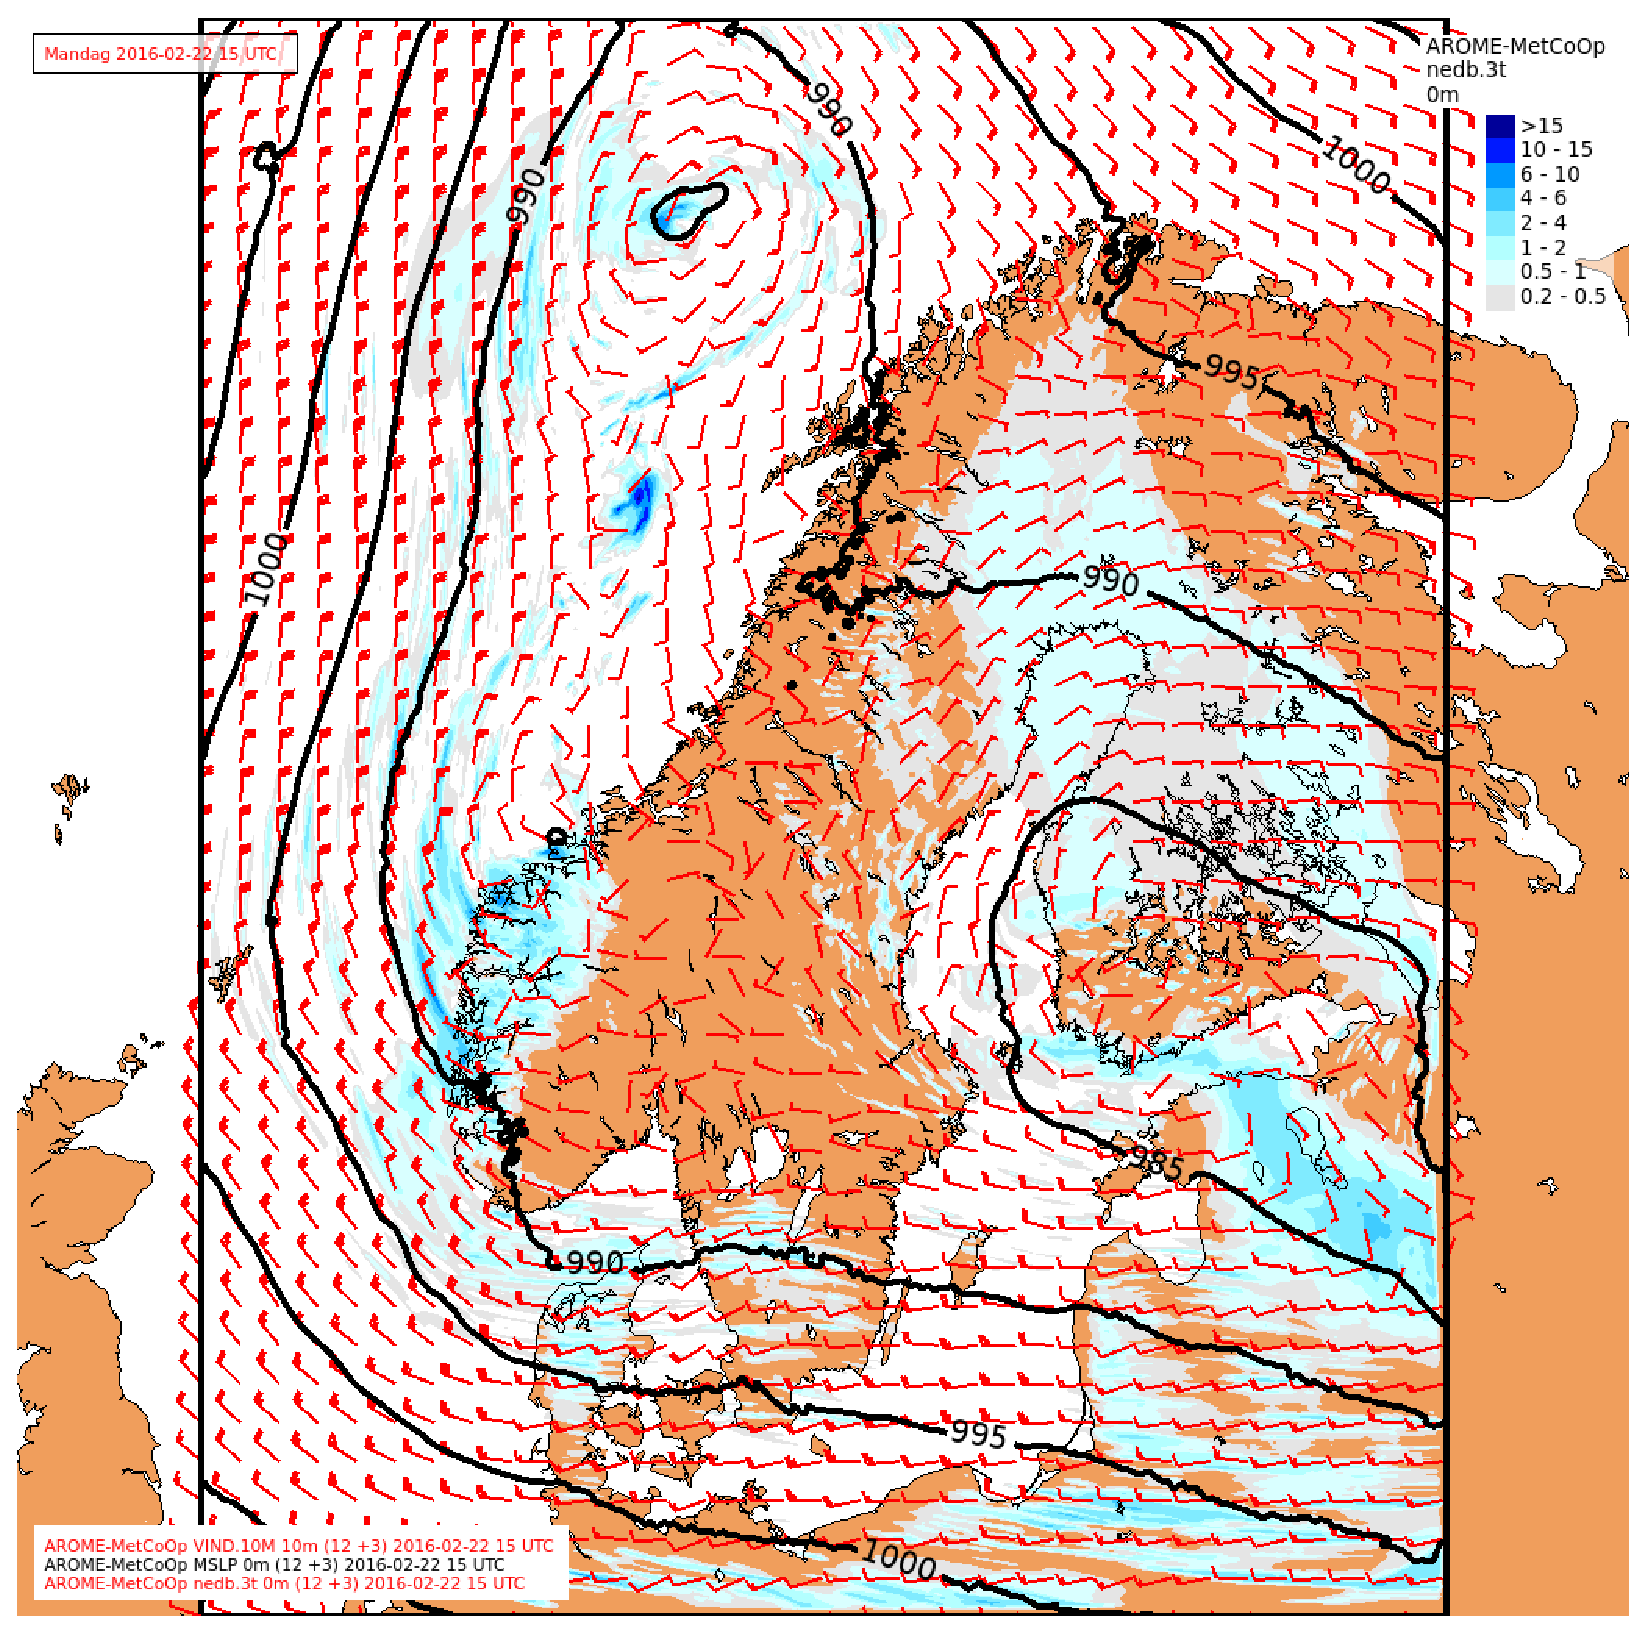
\includegraphics[height=10cm]{AROME_2016-02-22_15UTC}}
  \end{pspicture}
  \caption{\small The area covered by the Arome-MetCoop model. Shown is the forecasted (lead time 3 hrs) mean sea level pressure in hPa (black solid lines, countour interval = 5 hPa), 3 hourly precipitation, and 10 m wind valid at 1500UTC on February 22, 2016. Color bar indicates precipitation with a variable contour interval in the range 0.2-15 mm or larger (deep blue).} 
  \label{fig:arome}
 \end{center}
\end{figure}



We extract from AROME-MetCoOp, as listed in Table \ref{tab:atmos_para}, surface analysis and forecasts of wind, pressure, temperature, humidity and cloud cover daily at 00, 06, 12, 18 UTC. Rainfall rates was calculated by using the accumulated rainfall at +6 hours lead time. AROME-MetCoOp store all these parameters at its grid resolution. From these parameters and variables fluxes are computed using the internal bulk-flux routines in ROMS \citep[e.g.,][]{roed:deber:2004}. FjordOs CL also computes internally, from analytic expressions, net long wave radiation and short wave radiation.
\begin{table}[t]
 \begin{center}
  \caption{List of atmospheric forcing parameters.}
   \begin{tabular}{lccl}
   \hline
    					& ROMS			& 		\\
    Parameter name			& input name		& Unit		\\
   \hline
    10 m U wind component		& Uwind			& ms$^{-1}$	\\
    10 m V wind component 		& Vwind			& ms$^{-1}$	\\
    2 m air temperature			& T$_{air}$		& $^{\text{o}}$C	\\
    Mean sea level pressure		& P$_{air}$		& hPa		\\
    Total cloud cover			& cloud			& -		\\
    Specific humidity			& Q$_{air}$		& g kg$^{-1}$	\\
    Total precipitation			& rain			& kgm$^{-2}$s$^{-1}$		\\
   \hline
   \end{tabular}
  \label{tab:atmos_para}
 \end{center}
\end{table} 



% % % % % % % % % % % % % % % % % % % % % % % % % % % % % % % % 
\subsection{Input at open lateral boundaries}
\label{subsec:lateral}

%    %    %    %    %    %    %    %    %    %    %    %    %   
\subsubsection{De-tided input}
\label{subsubsec:detid}
The FjordOs CL grid has one wide open boundary located at its southern end towards the Skagerrak. Here we use input from the NorKyst800 model in the form of daily mean (de-tided) values of sea level, currents and hydrography. The NorKyst800 model covers the Norwegian coast including the Skagerrak and the Oslofjord with a grid resolution of 800 m as shown by Figure \ref{fig:n800}. To include the forcing from the NorKyst800 model a one-way nesting technique is employed as described in \cite{march:etal:2001}.  

The NorKyst800 is run operationally at MET Norway once a day and provides hourly forecasts with a lead time of 66 hrs. Daily mean values are computed and stored as netCDF files. These fields with some modifications may in addition be used as initial values to "semi-hot" start FjordOs (Section \ref{sec:resul}). The archive containing daily mean values is updated automatically and adds back to 2012. The hourly forecast values are stored and archived one week back in time only. Both archives are available from MET Norway's thredds server\footnote{\texttt{http://thredds.met.no/thredds/fou-hi/norkyst800m.html}}. As input at the lateral open boundary FjordOs CL requires daily mean sea level values in addition to daily mean depth profiles of currents temperature and salinity.

%    %    %    %    %    %    %    %    %    %    %    %    %   
\subsubsection{Tidal forcing}
\label{subsubsec:tides}
The daily mean values extracted from NorKyst800 are viewed as being crudely de-tided. To get tides into the FjordOs CL model, tidal elevation and tidal (barotropic) currents have to be specified separately and superimposed on the daily mean NorKyst800 input. 
%%%%%%%%%%%%%%%%%%%%%%%%%%% Tidal componetns %%%%%%%%%%%%%%%%%%%%%%%%%%%%%%%%%%%%%%
%\clearpage
\begin{table}[t]
 \caption{Simulated tidal amplitudes [cm] and phases [deg] for a location close to the Viker tidal gauge station. The column "ATPXO" refers to the simulated tides using the TPXO Atlantic data base as input, while the column "Modified" refers to a run using adjusted tides as input. The column "Observed" refers to the observed tides at the nearby Viker tidal gauge station and is added for comparison.}
 \label{tab:1}
 \centering
 \newcolumntype{+}{D{+}{\pm}{2}}
% \begin{tabular}{|c|r|++|++|++|} 
 \begin{tabular}{cr++++++} 
  \hline
  Con-    & \mc{1}{c}{Period}      & \mc{2}{c}{Observed}       & \mc{2}{c}{ATPXO}           & \mc{2}{c}{Modified}\\
  stit.   & \mc{1}{c}{[hrs]} 
                    & \mc{1}{c}{[cm]} 
                                   & \mc{1}{c}{[deg]} 
                                                & \mc{1}{c}{[cm]} 
                                                               & \mc{1}{c}{[deg]} 
                                                                             & \mc{1}{c}{[cm]} 
                                                                                            & \mc{1}{c}{[deg]}\\
  \hline
  M$_2$  & 12.4206 & 12.4+0.7 & 115+3  &  9.7+1.1 & 122+6   & 11.8+0.3 & 105+1  \\
  N$_2$  & 12.6583 &  2.8+0.7 &  69+14 &  5.7+1.1 &  81+11  &  3.1+0.3 &  69+5  \\
  S$_2$  & 12.0000 &  2.3+0.7 &  48+15 &  5.1+1.0 &  81+11  &  3.2+0.3 &  67+5  \\
  O$_1$  & 25.8193 &  2.1+0.7 & 282+20 &  3.7+0.4 &  19+8   &  2.9+0.2 & 338+3  \\
  M$_4$  &  6.2103 &  1.4+0.2 & 287+7  &  0.7+0.2 &  25+17  &  1.1+0.0 & 354+1  \\
  Q$_1$  & 26.8684 &  1.0+0.6 & 221+42 &  0.1+0.3 & 215+154 &  0.1+0.1 & 253+156\\
  K$_1$  & 23.9345 &  0.7+0.6 &  98+49 &  1.2+0.5 & 212+23  &  0.1+0.1 & 198+97 \\
  MN$_4$ &  6.2692 &  0.4+0.2 & 270+24 &  1.0+0.2 & 141+12  &  0.3+0.0 &   7+3  \\
  MS$_4$ &  6.1033 &  0.4+0.2 &   5+28 &  1.1+0.2 & 111+12  &  0.6+0.0 &  80+1  \\
   \hline
 \end{tabular}
\end{table}




The tidal input in terms of tidal elevations and currents are based on the TPXO Atlantic database \citep[][hereafter ATPXO]{egber:erofe:2002}\footnote{\texttt{http://volkov.oce.orst.edu/tides/AO.html}}. Before supplying them to the FjordOs CL model they were first modified using measured tides at the Viker tidal gauge station located close to the southern boundary in the Hvaler Archipelago. Included are the nine tidal constituents listed in Tables \ref{tab:1} and \ref{tab:2}. As is evident semi-diurnal constituent M$_2$ is by far the most dominant one, but also N$_2$ and S$_2$ contributes. 
\begin{table}[t]
%\vspace{-1.5cm}
  \caption{As Table \ref{tab:1}, but for the Oscarsborg tidal gauge station.}
  \label{tab:2}
  \centering
 \newcolumntype{+}{D{+}{\pm}{2}}
 \begin{tabular}{cr++++++} 
  \hline
  Con-    & \mc{1}{c}{Period}      & \mc{2}{c}{Observed}       & \mc{2}{c}{ATPXO}           & \mc{2}{c}{Modified}\\
  stit.   & \mc{1}{c}{[hrs]} 
                    & \mc{1}{c}{[cm]} 
                                   & \mc{1}{c}{[deg]} 
                                                & \mc{1}{c}{[cm]} 
                                                               & \mc{1}{c}{[deg]} 
                                                                             & \mc{1}{c}{[cm]} 
                                                                                            & \mc{1}{c}{[deg]}\\
  \hline
  M$_2$   & 12.4206 & 14.1+0.7 & 132+3  & 11.1+1.2 & 128+7   & 13.7+0.3 & 111+2      \\
  N$_2$   & 12.6583 &  3.0+0.8 &  85+15 &  6.6+1.4 &  86+10  &  3.6+0.4 &  75+6      \\
  S$_2 $  & 12.0000 &  2.7+0.8 &  70+18 &  6.1+1.3 &  85+11  &  3.7+0.4 &  70+7      \\
  O$_1$   & 25.8193 &  2.1+0.7 & 286+17 &  3.9+0.5 &  21+8   &  3.1+0.2 & 340+4      \\
  M$_4$   &  6.2103 &  2.1+0.3 & 332+8  &  1.4+0.4 &  44+19  &  2.0+0.0 &  14+1      \\
  Q$_1$   & 26.8684 &  1.0+0.7 & 230+36 &  0.2+0.4 & 204+126 &  0.0+0.2 & 190+165    \\
  K$_1$   & 23.9345 &  1.2+0.5 & 101+35 &  1.1+0.5 & 213+27  &  0.1+0.2 &  44+79     \\
  MN$_4$  &  6.2692 &  0.6+0.3 & 316+26 &  2.0+0.4 & 163+14  &  0.5+0.0 &  29+3      \\
  MS$_4$  &  6.1033 &  0.5+0.3 &  57+32 &  2.2+0.4 & 135+11  &  1.3+0.0 & 106+1      \\
  \hline
 \end{tabular}
\end{table}





The rationale for the modification of the tidal input is that the resolution of the ATPXO, which is 1/30$^{\textrm{o}}$, is too coarse to get the exact phase and amplitude of the tides in Skagerrak correct. To modify the tides we first imposed the nine constituents on the open boundary of tides from the ATPXO database, and let it run for more than a year (the actual period was 12:00 UTC, April 1, 2014 - 12:00 UTC, September 28, 2014). Time series of water level from a location near the Viker and Oscarsborg tidal gauge stations were then extracted and analyzed based on the T\_Tide package described by \cite{pavlo:etal:2002}. The results are shown under column ``ATPXO'' in Tables \ref{tab:1} and \ref{tab:2}. For comparison we have also extracted and analyzed the observed time series from the Viker and Oscarsborg tidal gauge stations compiled from the Norwegian Coastal Administration (Tidevannstabeller for den norske kyst med Svalbard, 2008). The result of this analysis is shown in column ``Observed'', and clearly show that the simulated tides off the mark.  

To better match the observations tidal amplitudes and corresponding phases at the Viker tidal gauge station were then modified by computing an amplitude factor, $c^{(n)}$, and a phaseshift, $\Delta\phi^{(n)}$ for each tidal component $n$ according to:
\beq
  c^{(n)} &=& a^{(n)}_{obs} / a^{(n)}_{sim} \\
  \Delta \phi^{(n)} &=& \phi^{(n)}_{obs} - \phi^{(n)}_{sim}
\eeq
where $a^{(n)}$ is the amplitude and $\phi^{(n)}$ is the phase for tidal component number $n$ of the water level in the column ``ATPXO''. New amplitudes and phases at the boundary were then calculated using the computed amplification factor and phaseshift on both water level and velocity. The modified tides were then supplied to the FjordOs CL and run for a year with tidal forcing only. The new results were then analyzed exactly as for the ATPXO run. The resulting new tidal amplitudes and periods for the locations close to the Viker and Oscarsborg tidal gauge stations are shown in Tables \ref{tab:1} and \ref{tab:2} in column ``Modified''. The results are clearly improved at both stations. In particular we are pleased with the results close to the Oscarsborg tidal gauge station which may be viewed as a control station in that it is far away from the southern boundary where the tidal forcing is imposed.  



%  %  %  %  %  %  %  %  %  %  %  %  %  %  %  %  %  %  %  %  %  
\subsection{River input}
\label{subsec:river}
The influence of the freshwater discharged to the Oslofjord by way of the many rivers surrounding it is well known. A relevant example is shown by Figure \ref{fig:salt_hele} constructed from a test run with an earlier version of the FjordOs CL model. In particular the impact on the daily mean sea surface salinity of Norway's two largest rivers, namely Glomma to the southeast and Drammenselva to the northwest, is evident. As shown it tends to create salinity fronts that in turn give rise to high lateral as well as vertical shear currents. From time to time these fronts are even strong enough to generate instabilities. To obtain a realistic, high resolution picture of the circulation in the Oslofjord it is therefore paramount to include the input from these and other smaller rivers.
% %%%%%%%%%%%%%%%%%%%%%%%%%% Figure 1 Oversiktskart %%%%%%%%%%%%%%%%%%%%%%%%%%%%
\begin{figure}[t]
 \setlength{\unitlength}{1.0cm}
 \begin{center}
  \begin{pspicture}(0,0)(15,9)
% Include graphs
   \rput[bl](0,0){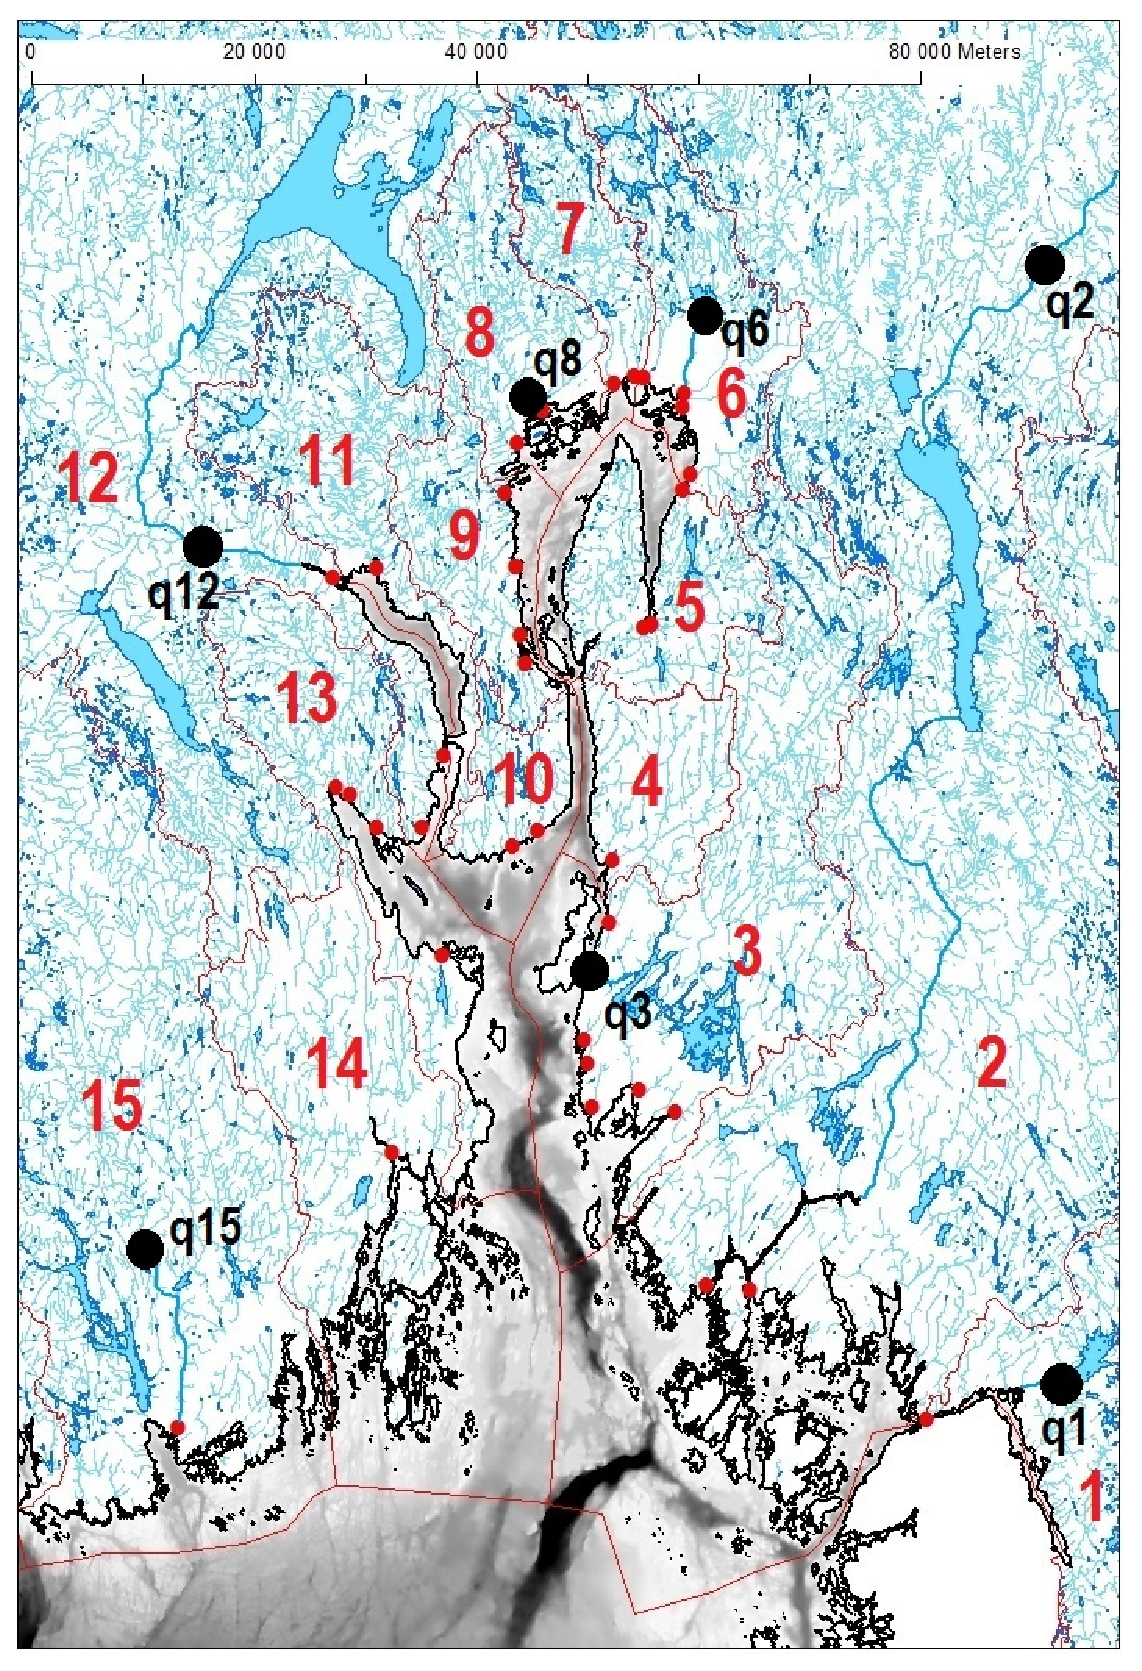
\includegraphics[height=9cm]{Elver_Oslofjorden_v4}}
   \rput[br](15,0){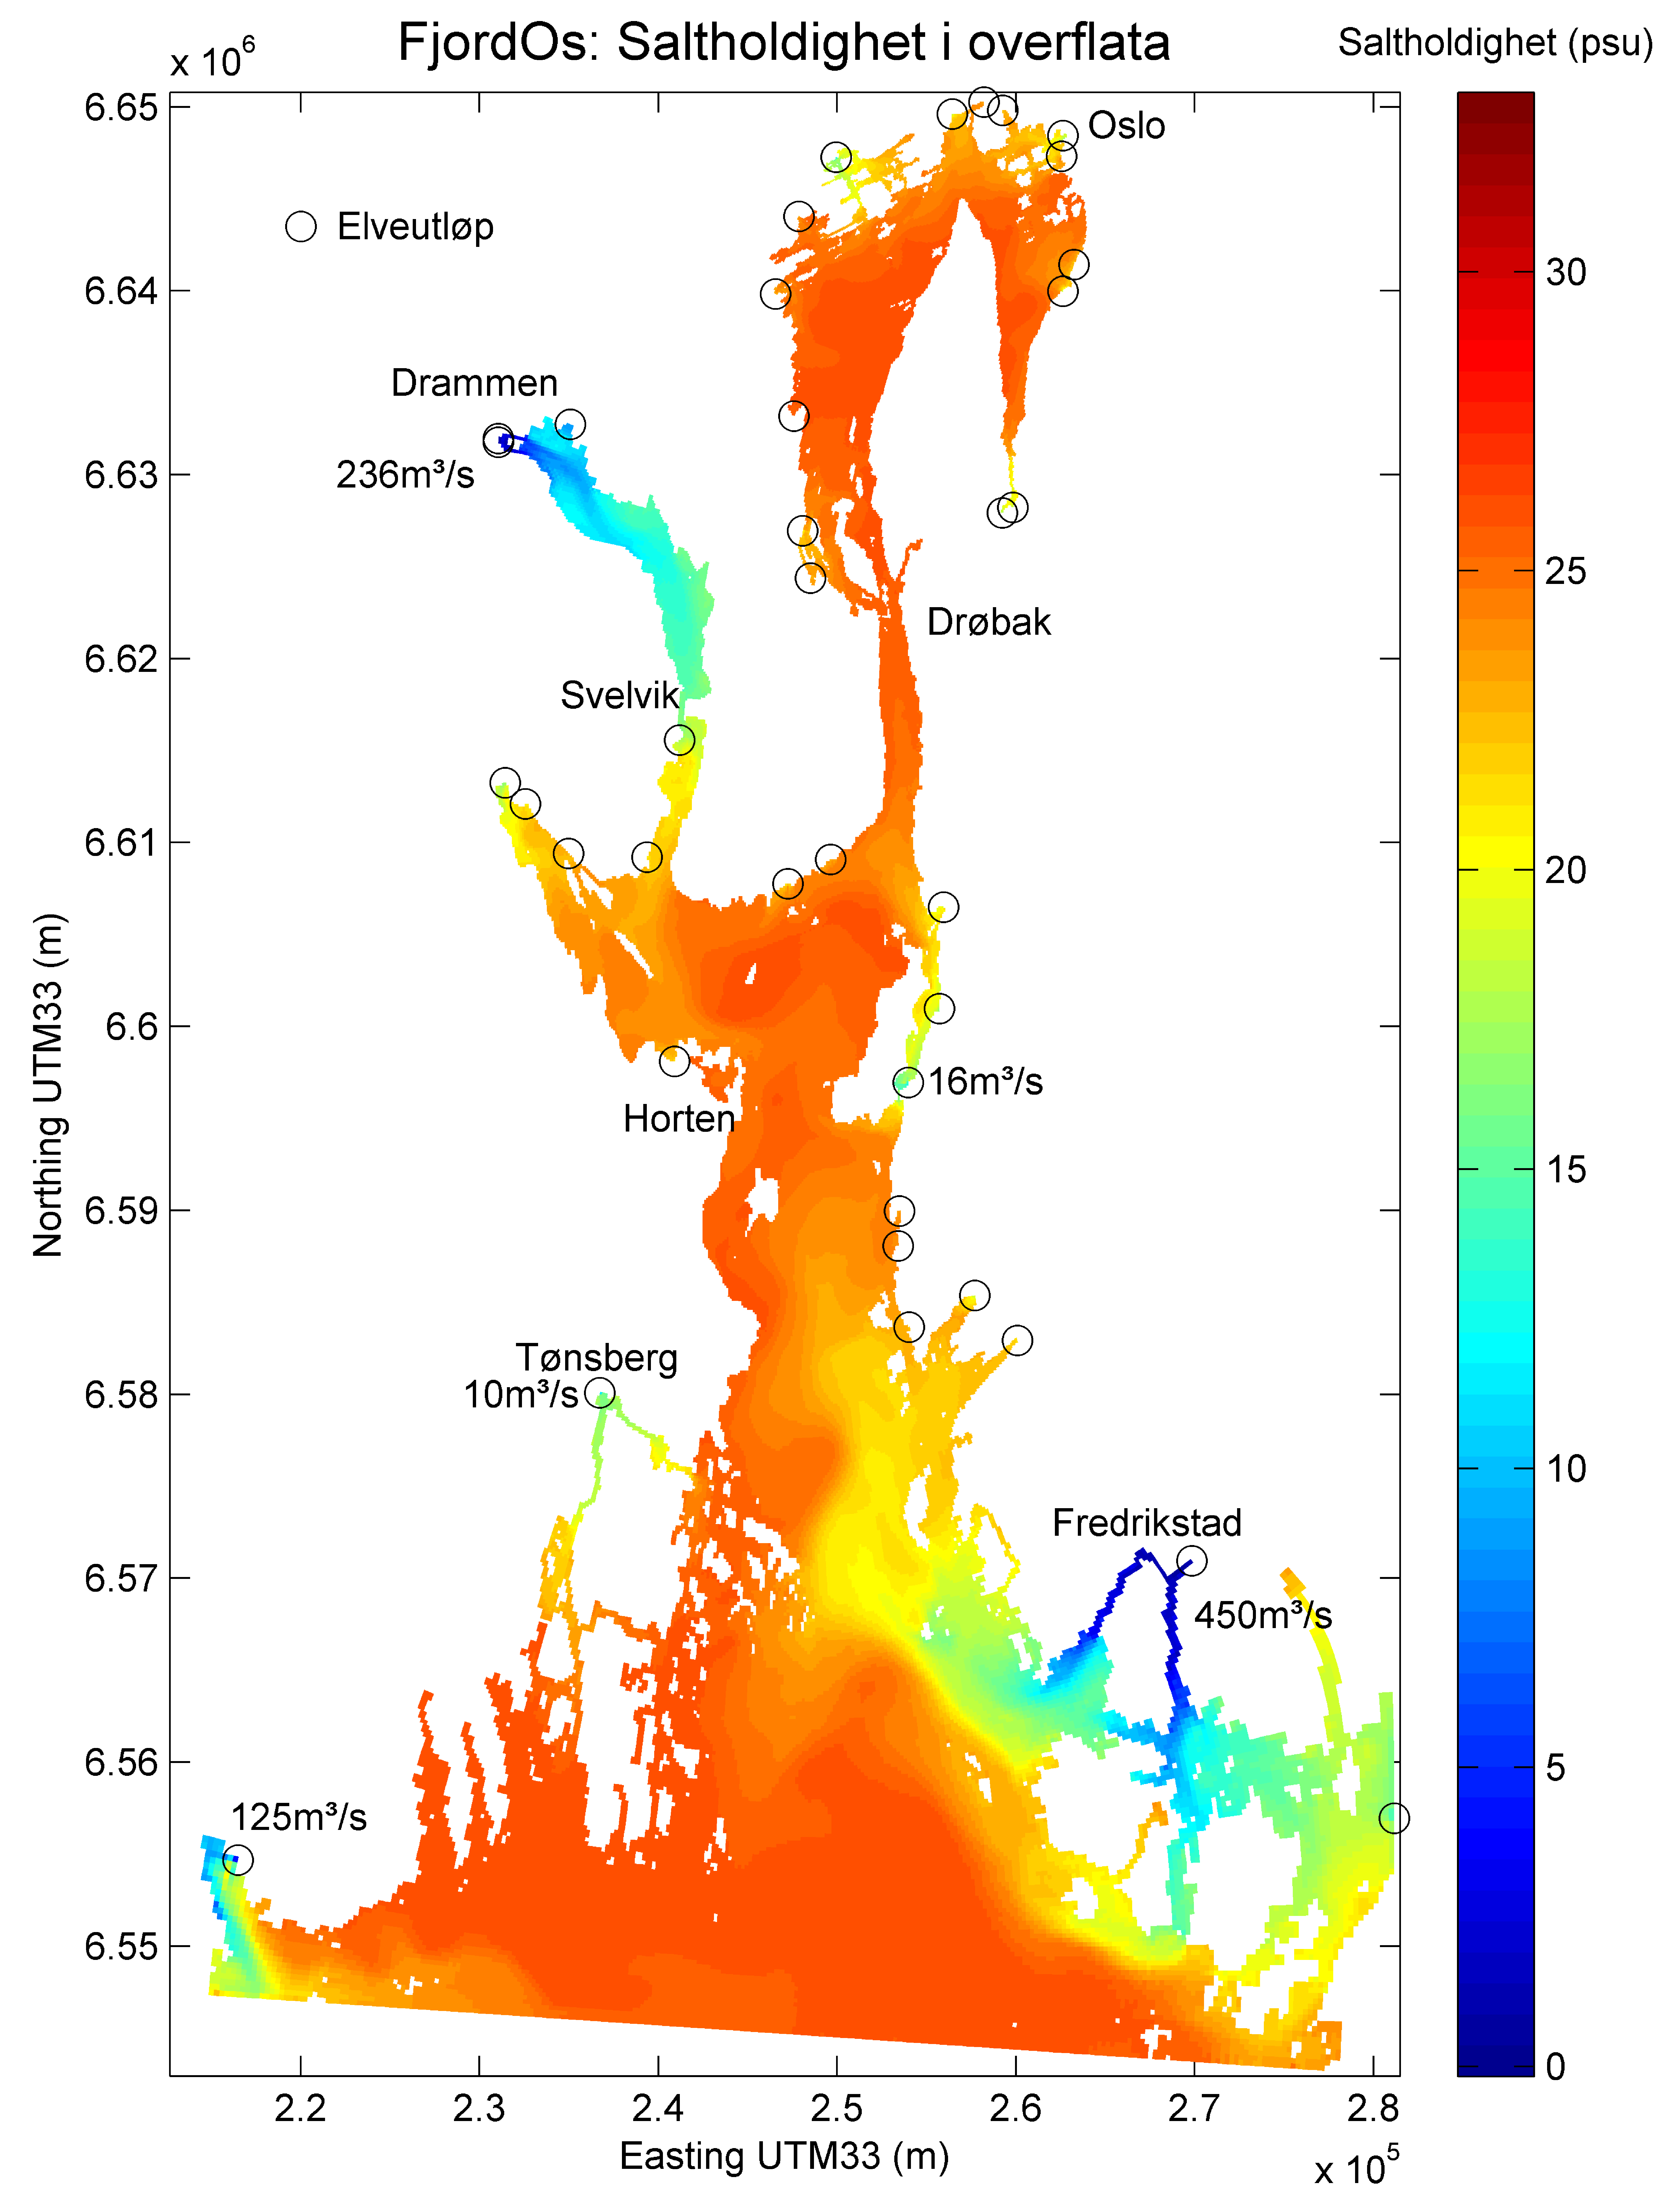
\includegraphics[height=9cm]{fjordos_rivers}}
  \end{pspicture}
% Figure caption is below the figure
  \caption{Left panel shows the many rivers (blue solid lines) emptying freshwater to the fjord (from NVE elvenett). The red numbers indicate a Main Catchment Area (MCA). The red dots indicate the location of the individual rivers discharging freshwater to Oslofjord (cf. Table \ref{tab:rivers01}). Some of the larger rivers, for instance Glomma, Drammenselva and Numedalsl{\aa}gen, are marked with a thicker blue line. Stations with water discharge measurements are shown with green dots and numbered with black numbers, e.g. q8. Right panel shows the location of the 37 rivers named in Table \ref{tab:rivers01}. }   
  \label{fig:rivers01}      
 \end{center}
\end{figure}
%

 

To obtain the necessary information on the freshwater discharges to the Oslofjord within the FjordOs CL model domain we make use of discharge data from a database constructed by use of the hydrological model HBV \citep{beldr:etal:2003}. In essence the HBV model provides an estimate of the daily mean freshwater drained into the ocean (or fjord) from a preselected set of so called Main Catchment Areas (MCAs). Each MCA has in turn at least one or more rivers with an outlet to the sea. Let $Q_i$ be the daily mean freshwater discharged from the $i$th MCA and $A_i$ its area. Furthermore, let $q_{ij}$ be the discharge from the $j$th individual river associated with the $i$th MCA. Then assuming that $q_{ij}$ is entirely determined by the ratio of its local catchment area $a_{ij}$ to the area of the MCA, that is $A_i$ we get
\be
 \label{eq:riv02}
  q_{ij} = \frac{a_{ij}}{A_i} Q_i.
\ee

A total of 15 of Norway's MCAs drains into the Oslofjord within the FjordOs model domain (Figure \ref{fig:rivers01}). These MCAs in turn contain a total of 46 river outlets as listed by Table \ref{tab:rivers01}. Six of these belongs to Glomma and five to Drammenselva. Hence there are 37 named rivers. Their locations are shown by Figure \ref{fig:rivers01}. By use of (\ref{eq:riv02}) and Table \ref{tab:rivers01} we may find the discharge emitted from each of them provided $Q_i$ is known. The HBV database contains information on $Q_i$ from 1962 up to and including the previous year with a lag of about six months. Thus $Q_i$ was not available for 2015 at the time of the simulations presented in this report. Our hindcast period is from April 1, 2014 up to and including December 2015. We must therefore obtain information on $Q_i$ for 2015 from another source. To this end we make use of observations from the NVE website\footnote{\texttt{http://www2.nve.no/h/hd/plotreal/Q/index.html}} available in near real time. If we for instance consider the observed discharge from river $n$ within the $i$th MCA, we find $Q_i$ by rearranging (\ref{eq:riv02}), that is,
\be
 \label{eq:riv03}
  Q_i = A_i\frac{q_{in}}{a_{in}}.
\ee
where $q_{in}$ is the known discharge of the $n$'th river and $a_{in}$ is the size of its local catchment area. Having thus found $Q_i$ we find the discharges from the remaining rivers of that MCA by use of (\ref{eq:riv02}) and the $a_{ij}$'s listed in Table \ref{tab:rivers01}.

Using this method we first calculated the daily mean discharge for MCA numbers $i=1, 2, 3, 6, 8, 12$, and $15$ using the NVE station data for rivers nos. 1 (Iddefjorden/Haldenv.), 2-7 (Glomma), 13 (Mosseelva), 21 (Akerselva), no. 25 (Sandvikselva), 34-38 (Drammenselva) and 46 (Numedalsl{\aa}gen). The NVE station for MCA no. 2 is located far upriver (Figure \ref{fig:rivers01}), so a correction factor is estimated based on a least square fit between the NVE observations at R{\aa}n{\aa}sfoss and the Glommens og Laagens Brukseierforening (glb.no) observations at Sarpfoss for the period up to and including October 28, 2015. The result is
\be
 \label{eq:riv04}
 Q_2 = 1.123 \cdot Q_{\text{R{\aa}n{\aa}sfoss}}.
\ee
This yields an estimate of the river discharge in Glomma with an RMS error of about 100 m$^3$/s. The corresponding discharges, that is, $q_{2j}$ for $j=2,3,\ldots,7$, are found by use of (\ref{eq:riv02}) and the size of the corresponding local catchment areas $a_{2j}$ listed in Table \ref{tab:rivers01}.
%%%%%%%%%%%%%%%%%%%%%%%%%%% Location of rivers %%%%%%%%%%%%%%%%%%%%%%%%%%%%%%%%%%%%%%
\clearpage
\vspace{5mm}
\tablecaption{Rivers in the FjordOs CL model. The outlet positions follow the index convention in ROMS. The position is at a $u$-point if the direction is along the $x$-axis, and at a $v$-point if the direction is along the $y$-axis. The index counting in ROMS starts at 0, except for the $u$-points and $v$-points, where the count starts at 1. MCA: Main Catchment Area.}
\tablefirsthead{\hline 
  River	& MCA	& \mc{1}{c}{Area}	& Outlet	& Outlet	& Direction	& Sign	& Name			\\ 
  No.	& no.   & \mc{1}{c}{$a_{ij}$}	& $x$-pos.	& $y$-pos.	& 0=along $x$	&	&			\\
	&       &			&       	&       	& 1=along $y$	&	&			\\
		\hline }
\tablehead{\hline \mc{8}{l}{\small\slshape continued from previous page}  \\ \hline
  River	& MCA	& \mc{1}{c}{Area}	& Outlet	& Outlet	& Direction	& Sign	& Name			\\ 
  No.	& no.   & \mc{1}{c}{$a_{ij}$}	& $x$-pos.	& $y$-pos.	& 0=along $x$	&	&			\\
	&       &			&       	&       	& 1=along $y$	&	&			\\
		\hline}
\tabletail{\hline \mc{8}{r}{\small\slshape continued on next page}  \\ \hline}
\tablelasttail{\hline}
\begin{center}
% \newcolumntype{d}{D{.}{.}{2}}
 \begin{supertabular}{ccrccccl}
  1	& 1	& 2512.00	& 297		& 44		& 0		& -1	& Iddefjorden/Haldenv.		\\
  2	& 2	& 7222.43	& 261		& 77		& 1		& -1	& Glomma ({\O}sterelva)		\\
  3	& 2	& 7222.43	& 260		& 77		& 1		& -1	& Glomma ({\O}sterelva)		\\
  4	& 2	& 7222.43	& 259		& 77		& 1		& -1	& Glomma ({\O}sterelva)		\\
  5	& 2	& 7222.43	& 258		& 70		& 1		& -1	& Glomma ({\O}sterelva)		\\
  6	& 2	& 7114.64	& 248		& 91		& 0		& -1	& Glomma (Vesterelva)		\\
  7	& 2	& 7114.64	& 248		& 92		& 0		& -1	& Glomma (Vesterelva)		\\
  8	& 3	& 13.90		& 273		& 202		& 0		& -1	& Krokstadbekken		\\
  9	& 3	& 25.90		& 251		& 230		& 1		& -1	& Heiabekken+Kure{\aa}a		\\
  10	& 3	& 7.57		& 213		& 219		& 1		& -1	& St{\o}tvikbekken		\\
  11	& 3	& 3.83		& 211		& 258		& 1		& +1	& Evje{\aa}a			\\
  12	& 3	& 5.55		& 213		& 275		& 1		& -1	& Gunnarbybekken		\\
  13	& 3	& 688.34	& 221		& 337		& 0		& -1	& Mossevassdraget		\\
  14	& 3	& 19.33		& 239		& 373		& 0		& -1	& Kambobekken			\\
  15	& 4	& 138.49	& 242		& 423		& 0		& -1	& H{\ae}lenelva			\\
  16	& 5	& 6.94		& 273		& 634		& 1		& +1	& Gloslibekken			\\
  17	& 5	& 51.72		& 280		& 638		& 1		& +1	& {\AA}rungelva			\\
  18	& 5	& 85.97		& 286		& 784		& 0		& -1	& Gjersj{\o}elva		\\
  19	& 6	& 39.10		& 289		& 802		& 0		& -1	& Ljanselva			\\
  20	& 6	& 69.26		& 267		& 864		& 0		& -1	& Alna				\\
  21	& 6	& 237.81	& 266		& 876		& 1		& -1	& Akerselva                	\\
  22	& 6	& 23.24		& 226		& 890		& 1		& -1	& Frognerbekken            	\\
  23	& 7	& 14.46		& 213		& 895		& 0		& -1	& Hoffelva               	\\
  24	& 7	& 176.30	& 188		& 888		& 1		& -1	& Lysakerelva                	\\
  25	& 8	& 227.72	& 83		& 843		& 1		& -1	& Sandvikselva                 	\\
  26	& 8	& 21.74		& 72		& 782		& 1		& -1	& Neselva			\\
  27	& 9	& 37.63		& 84		& 726		& 1		& +1	& Askerelva                   	\\
  28	& 9	& 2.82		& 126		& 665		& 1		& +1	& N{\ae}rsneselva		\\
  29	& 9	& 112.95	& 149		& 607		& 0		& +1	& {\AA}rosvassdraget		\\
  30	& 9	& 19.05		& 158		& 584		& 0		& +1	& S{\ae}treelva               	\\
  31	& 10	& 18.01		& 179		& 447		& 1		& -1	& Tofteelva			\\
  32	& 10	& 35.47		& 156		& 435		& 1		& -1	& Sageneelva			\\
  33	& 11	& 309.38	& 22		& 621		& 1		& -1	& Lierelva			\\
  34	& 12	& 2139.31	& 1		& 611		& 0		& +1	& Drammeneslva 1		\\
  35	& 12	& 4278.61	& 1		& 610		& 0		& +1	& Drammenselva 2		\\
  36	& 12	& 4278.61	& 1		& 609		& 0		& +1	& Drammenselva 3		\\
  37	& 12	& 4278.61	& 1		& 608		& 0		& +1	& Drammenselva 4		\\
  38	& 12	& 2139.31	& 1		& 607		& 0		& +1	& Drammeneslva 5		\\
  39	& 12	& 8.11		& 97		& 501		& 1		& -1	& Ebbestadelva   		\\
  40	& 12	& 14.54		& 82		& 447		& 0		& +1	& Bergerelva    		\\
  41	& 13	& 6.59		& 42		& 450		& 1		& -1	& Sandobekken    		\\
  42	& 13	& 29.84		& 22		& 472		& 1		& -1	& Selvikelva  			\\
  43	& 13	& 193.23	& 13		& 481		& 1		& -1	& Sandevassdraget   		\\
  44	& 13	& 33.66		& 93		& 351		& 1		& +1	& Borreelva       		\\
  45	& 14	& 1115.00	& 61		& 186		& 0		& +1	& Aulivassdraget      		\\
  46	& 15	& 6514.00	& 9		& 23		& 0		& -1	& Numedalsl{\aa}gen  		\\
 \end{supertabular}
\label{tab:rivers01}
\end{center}
\vspace{5mm}



For some of the 15 MCAs in the model domain, no observations are available ($i=$ 4, 5, 7, 9, 10, 11, 13, 14). We have estimated $Q_i$ for these rivers using the $Q_i$'s from MCA nos. 2 (Glomma), 3 (Mosseelva), 8 (Sandvikselva) and 15 (Nummedalsl{\aa}en). An auxiliary parameter was calculated that was the sum of the river discharges of all combinations of the four rivers. A least mean square fit was performed between this new parameter and the discharge for the MCA in question, namely 
\be
 \label{eq:riv05}
 Q_i = \alpha_i \left(f_{i2} Q_2 + f_{i3} Q_3 + f_{i8} Q_8 +f_{i15} Q_{15}\right) + \beta_i .
\ee
The result of this analysis is shown in Table \ref{tab:rivers04}. It is somewhat surprising that the discharge from MCA nos. 2 and 15 did not influence the estimate of the discharge from the other MCAs.   
%%%%%%%%%%%%%%%%%%%%%%%%%%% Summary of experiments %%%%%%%%%%%%%%%%%%%%%%%%%%%%%%%%%%%%%%
%\clearpage
\begin{table}[t]
 \caption{Estimating discharges in unobserved MCAs based on observations
 at four MCAs with observations using the least mean square fit (\ref{eq:riv05}).}
 \label{tab:rivers04}       % Give a unique label
% For LaTeX tables use
 \centering
% \begin{center}
   \begin{tabular}{ccccccc}
   \hline
   MCA & $f_{i2}$ & $f_{i3}$ & $f_{i8}$ & $f_{i15}$ & $\alpha_i$ & $\beta_i$  \\
   no. &          &          &          &           &            &            \\ 
   \hline
   4   & 0        &  1       &  0       &  0        & 0.201      &  0.120     \\
   5   & 0        &  1       &  0       &  0        & 0.265      &  0.274     \\
   7   & 0        &  0       &  1       &  0        & 0.625      &  0.531     \\
   9   & 0        &  0       &  1       &  0        & 0.750      &  0.209     \\
   10  & 0        &  0.5     &  0.5     &  0        & 0.264      & -0.276     \\
   11  & 0        &  0       &  1       &  0        & 1.317      &  0.417     \\
   13  & 0        &  0       &  1       &  0        & 1.081      &  0.998     \\
   14  & 0        &  0.5     &  0.5     &  0        & 1.000      &  1.087     \\
   \hline
   \end{tabular}
% \end{center}
\end{table}



Finally we emphasize that the rivers, in addition to providing freshwater to the fjord, are sources of nutrients, organic matter, bacteria, particles and contaminants. Several of these parameters are monitored in the national monitoring program \citep[Riverine Inputs and direct Discharges - RID,][]{skarb:etal:2011}. It is therefore possible to include information from the RID program in the river forcing, and hence the FjordOs CL model may be used in the future to model dispersion of any of the RID parameters.









\section{Results from test runs}
\label{sec:resul}
All the results shown below are derived by running FjordOs CL on the Vilje supercomputer at the Norwegian High Performance Computing facilities in Trondheim. We show results from a hindcast initialized from NorKyst800 on April 1st, 2014 and continued up to and including the month of December 2015. 
All inputs are as described in Section \ref{subsec:atmos}.
 
The results from the hindcast are further discussed and evaluated in some detail in an upcoming report \citep{hjelm:etal:2016}. Here we merely present snapshots of fields of currents, temperature, salinity and sea level so as to properly appreciate the level of details that the FjordOs CL model provides. In this we focus on six areas, namely the Inner Oslofjord, the Drammensfjord, the {\DR} area (henceforth {\DR}), the mid part of the Oslofjord (henceforth Slagen), the outer western part (henceforth Tristein) and the outer eastern part of the Oslofjord (henceforth Hvaler). 

\clearpage
%\subsubsection{Currents}
 %%%%%%%%%%%%%%%%%%% Figure  %%%%%%%%%%%%%%%
\begin{figure}[t]
  \begin{pspicture}(0,0)(15,12)
% Include graphs
	\rput[b](7.5,0){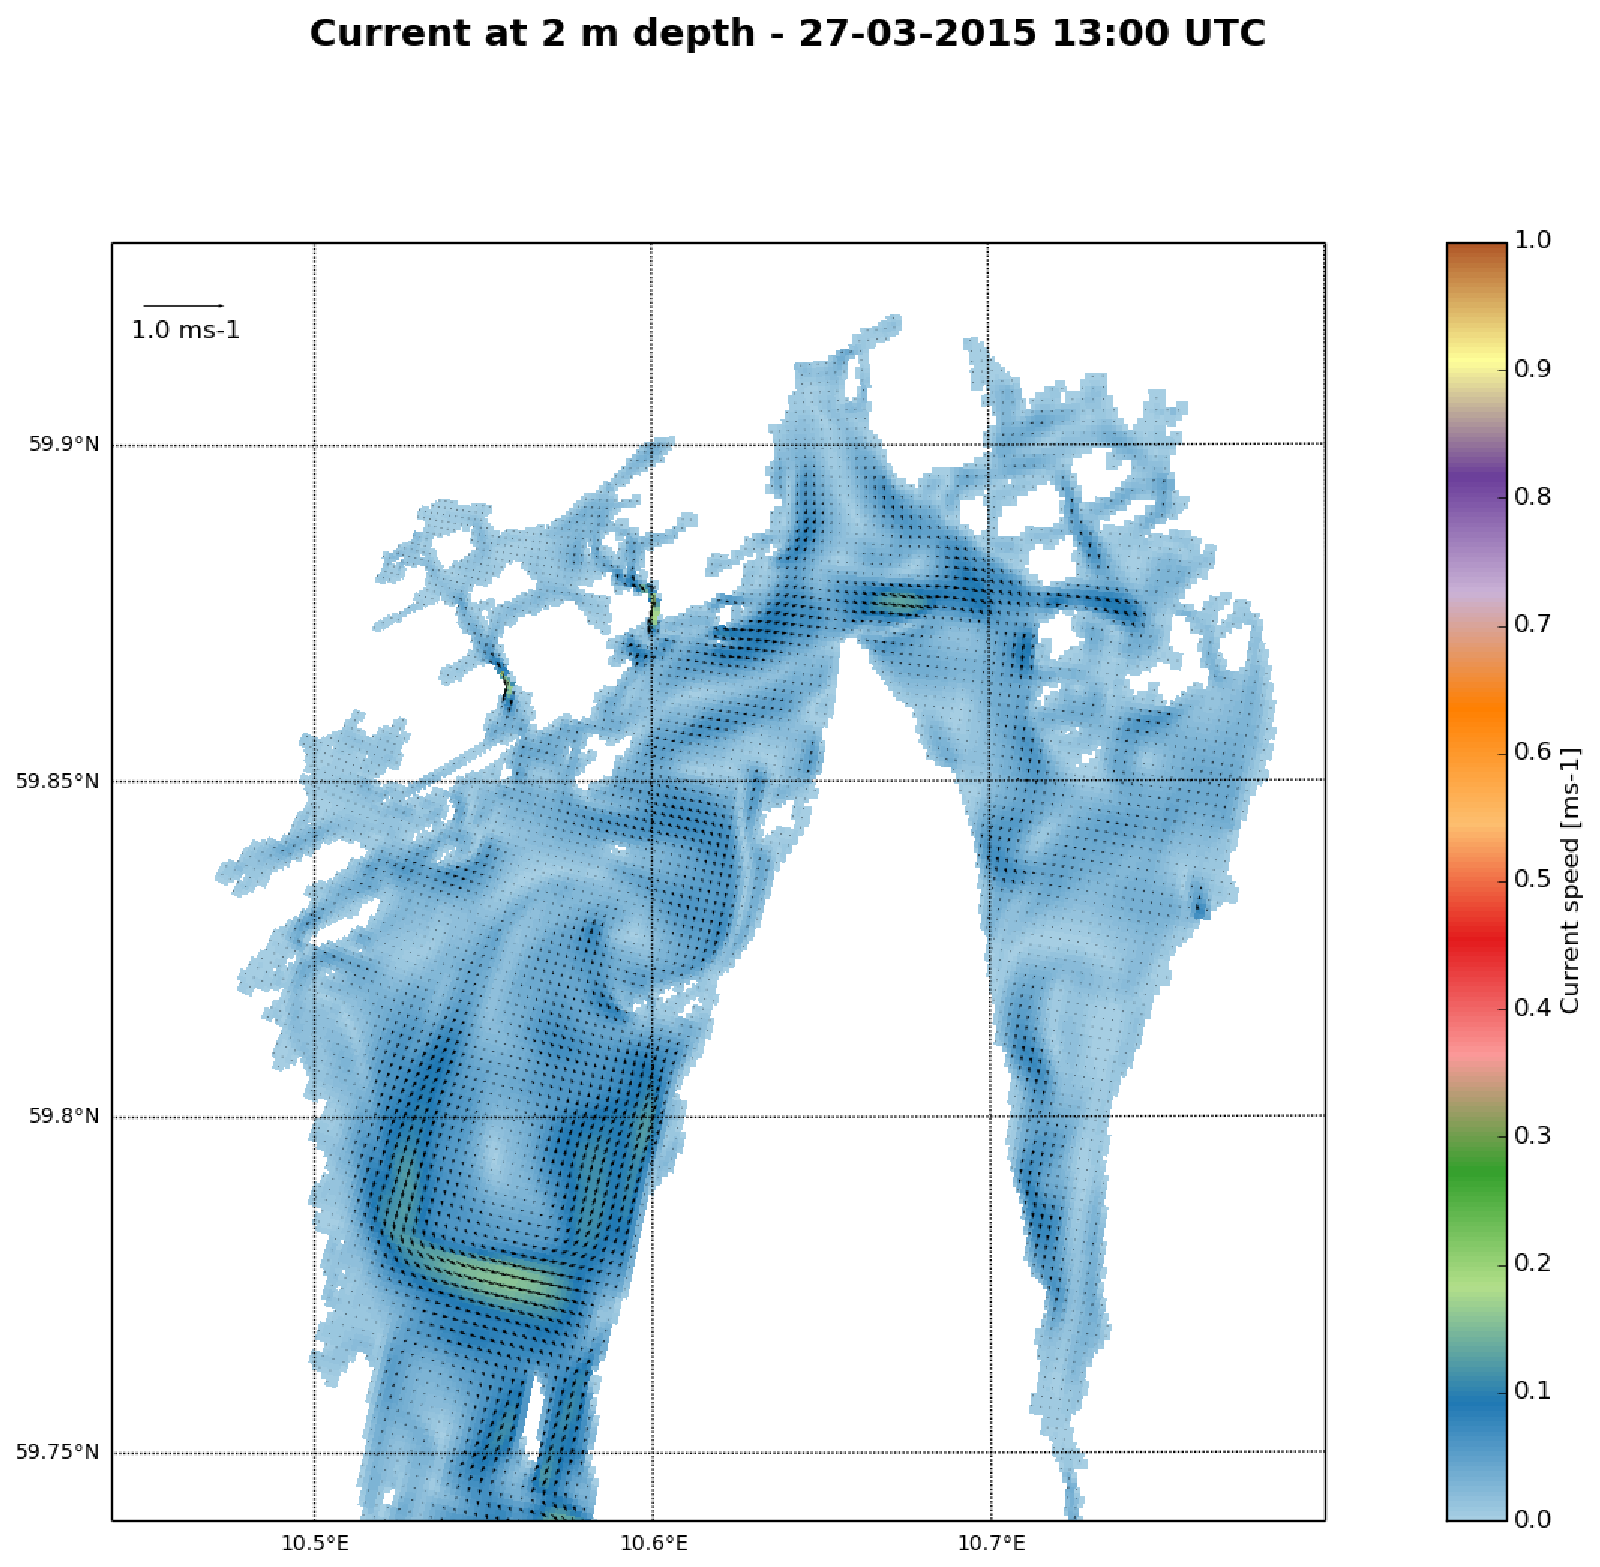
\includegraphics[height=12cm]{kap5/ferder1__0_current_crop}}
  \end{pspicture}
  \caption{\small  Currents .  }
  \label{fig:curr_oslo}
\end{figure}

  
 %%%%%%%%%%%%%%%%%%% Figure  %%%%%%%%%%%%%%%
\begin{figure}[t]
  \begin{pspicture}(0,0)(15,14)
% Include graphs
	\rput[b](7.5,-0.5){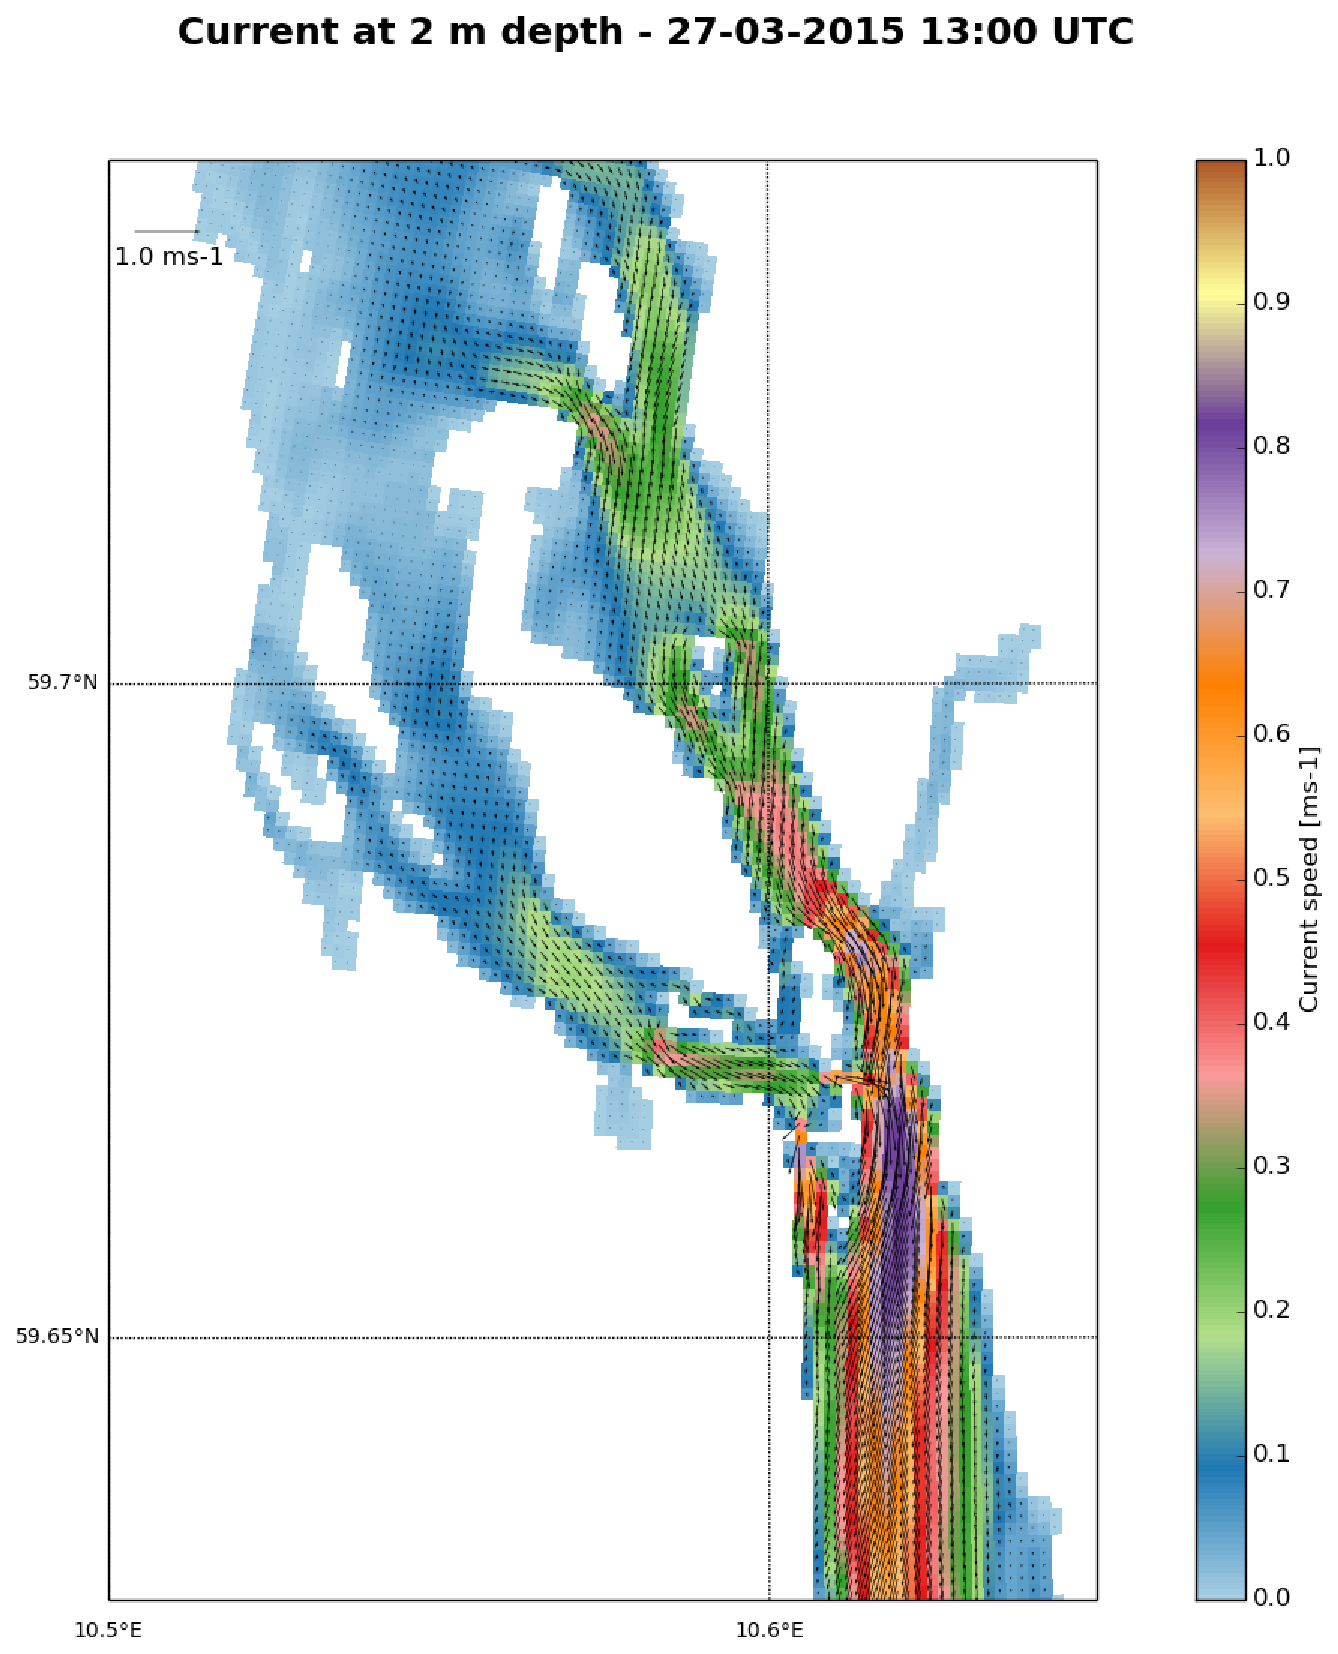
\includegraphics[height=14.5cm]{kap5/ferder2__0_current_crop}}
  \end{pspicture}
  \caption{\small As Figure \ref{fig:curr_oslo}, but for the Dr{\o}bak Sound and Vestfjorden area.}
  \label{fig:curr_drobak}
\end{figure}

  
 %%%%%%%%%%%%%%%%%%% Figure  %%%%%%%%%%%%%%%
\begin{figure}[t]
  \begin{pspicture}(0,0)(15,12)
% Include graphs
	\rput[b](7.5,0){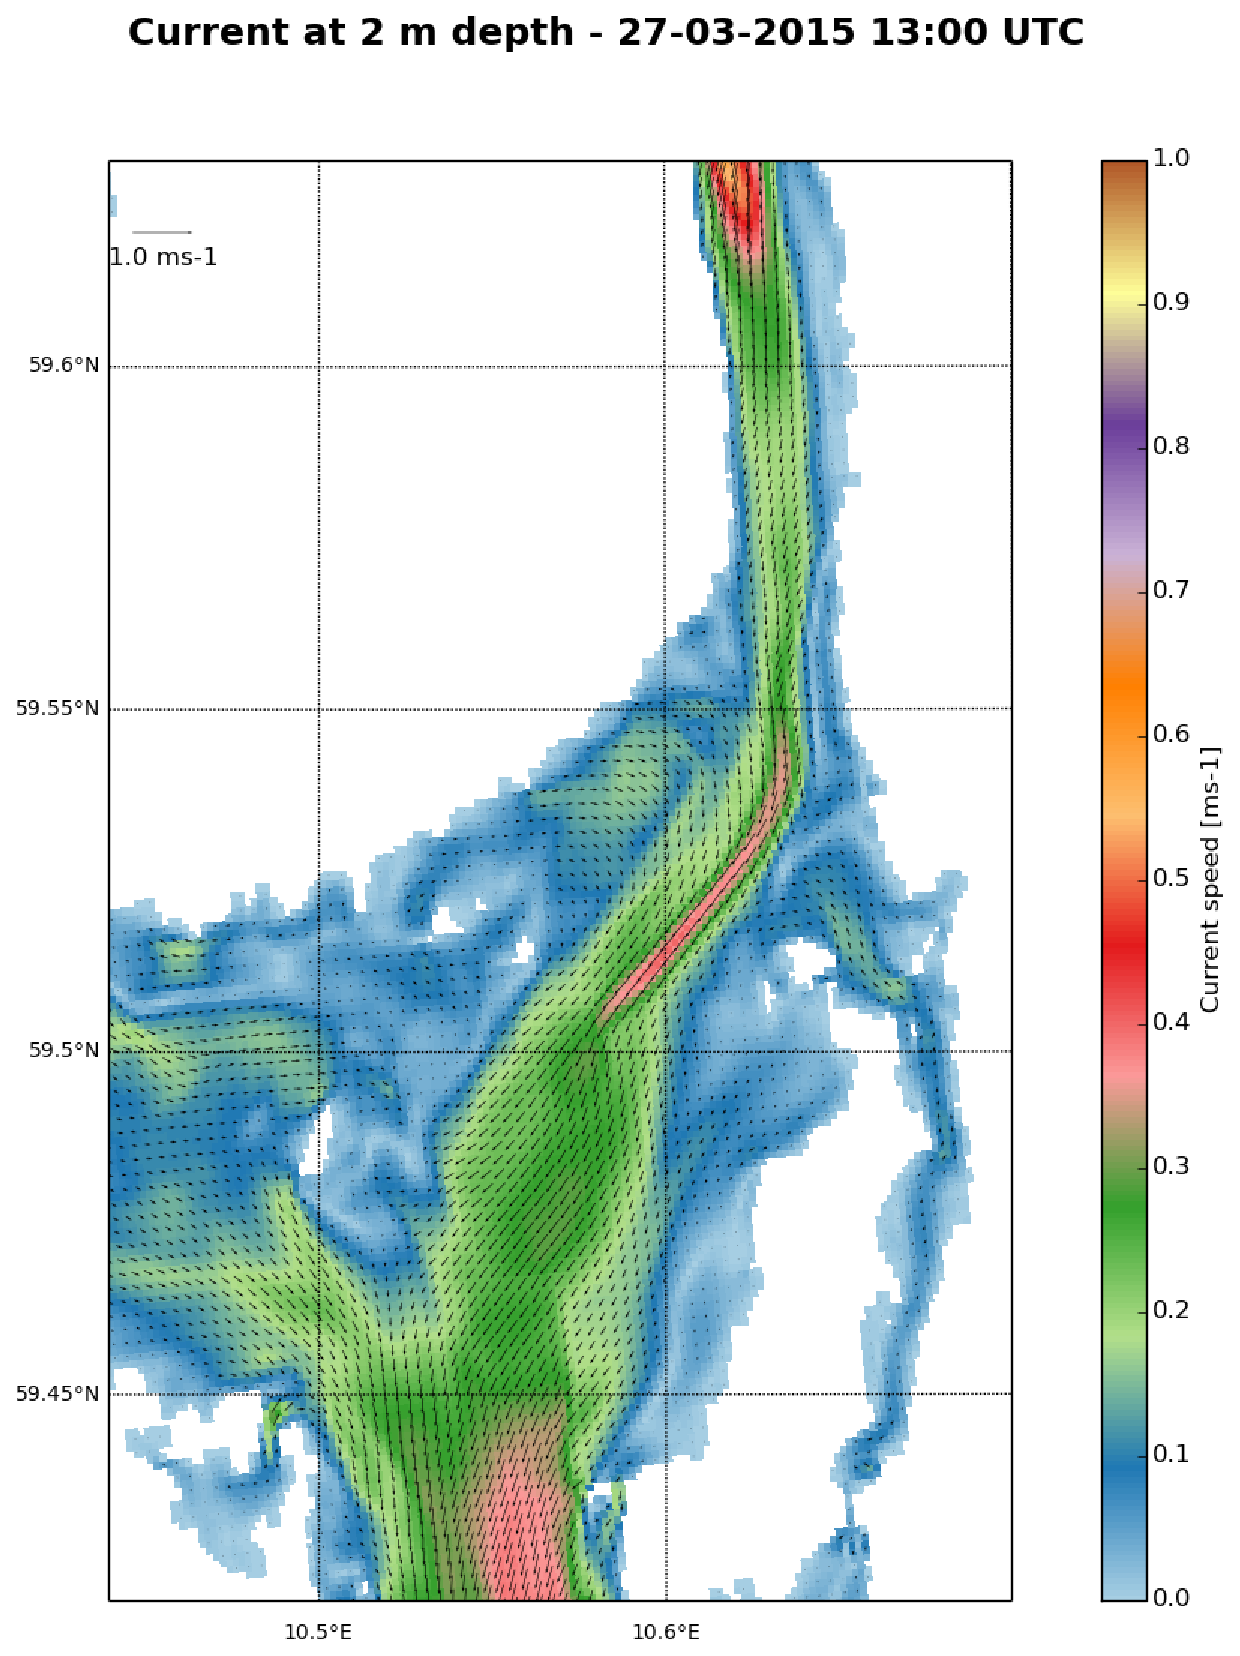
\includegraphics[height=12cm]{kap5/ferder3__0_current_crop}}
  \end{pspicture}
  \caption{\small  As for figure \ref{fig:curr_oslo}, but for the southern part of the Dr{\o}bakssund and Breidangen area.  }
  \label{fig:curr_breiangen}
\end{figure}

  
 %%%%%%%%%%%%%%%%%%% Figure  %%%%%%%%%%%%%%%
\begin{figure}[t]
  \begin{pspicture}(0,0)(15,16)
% Include graphs
	\rput[b](7.5,0){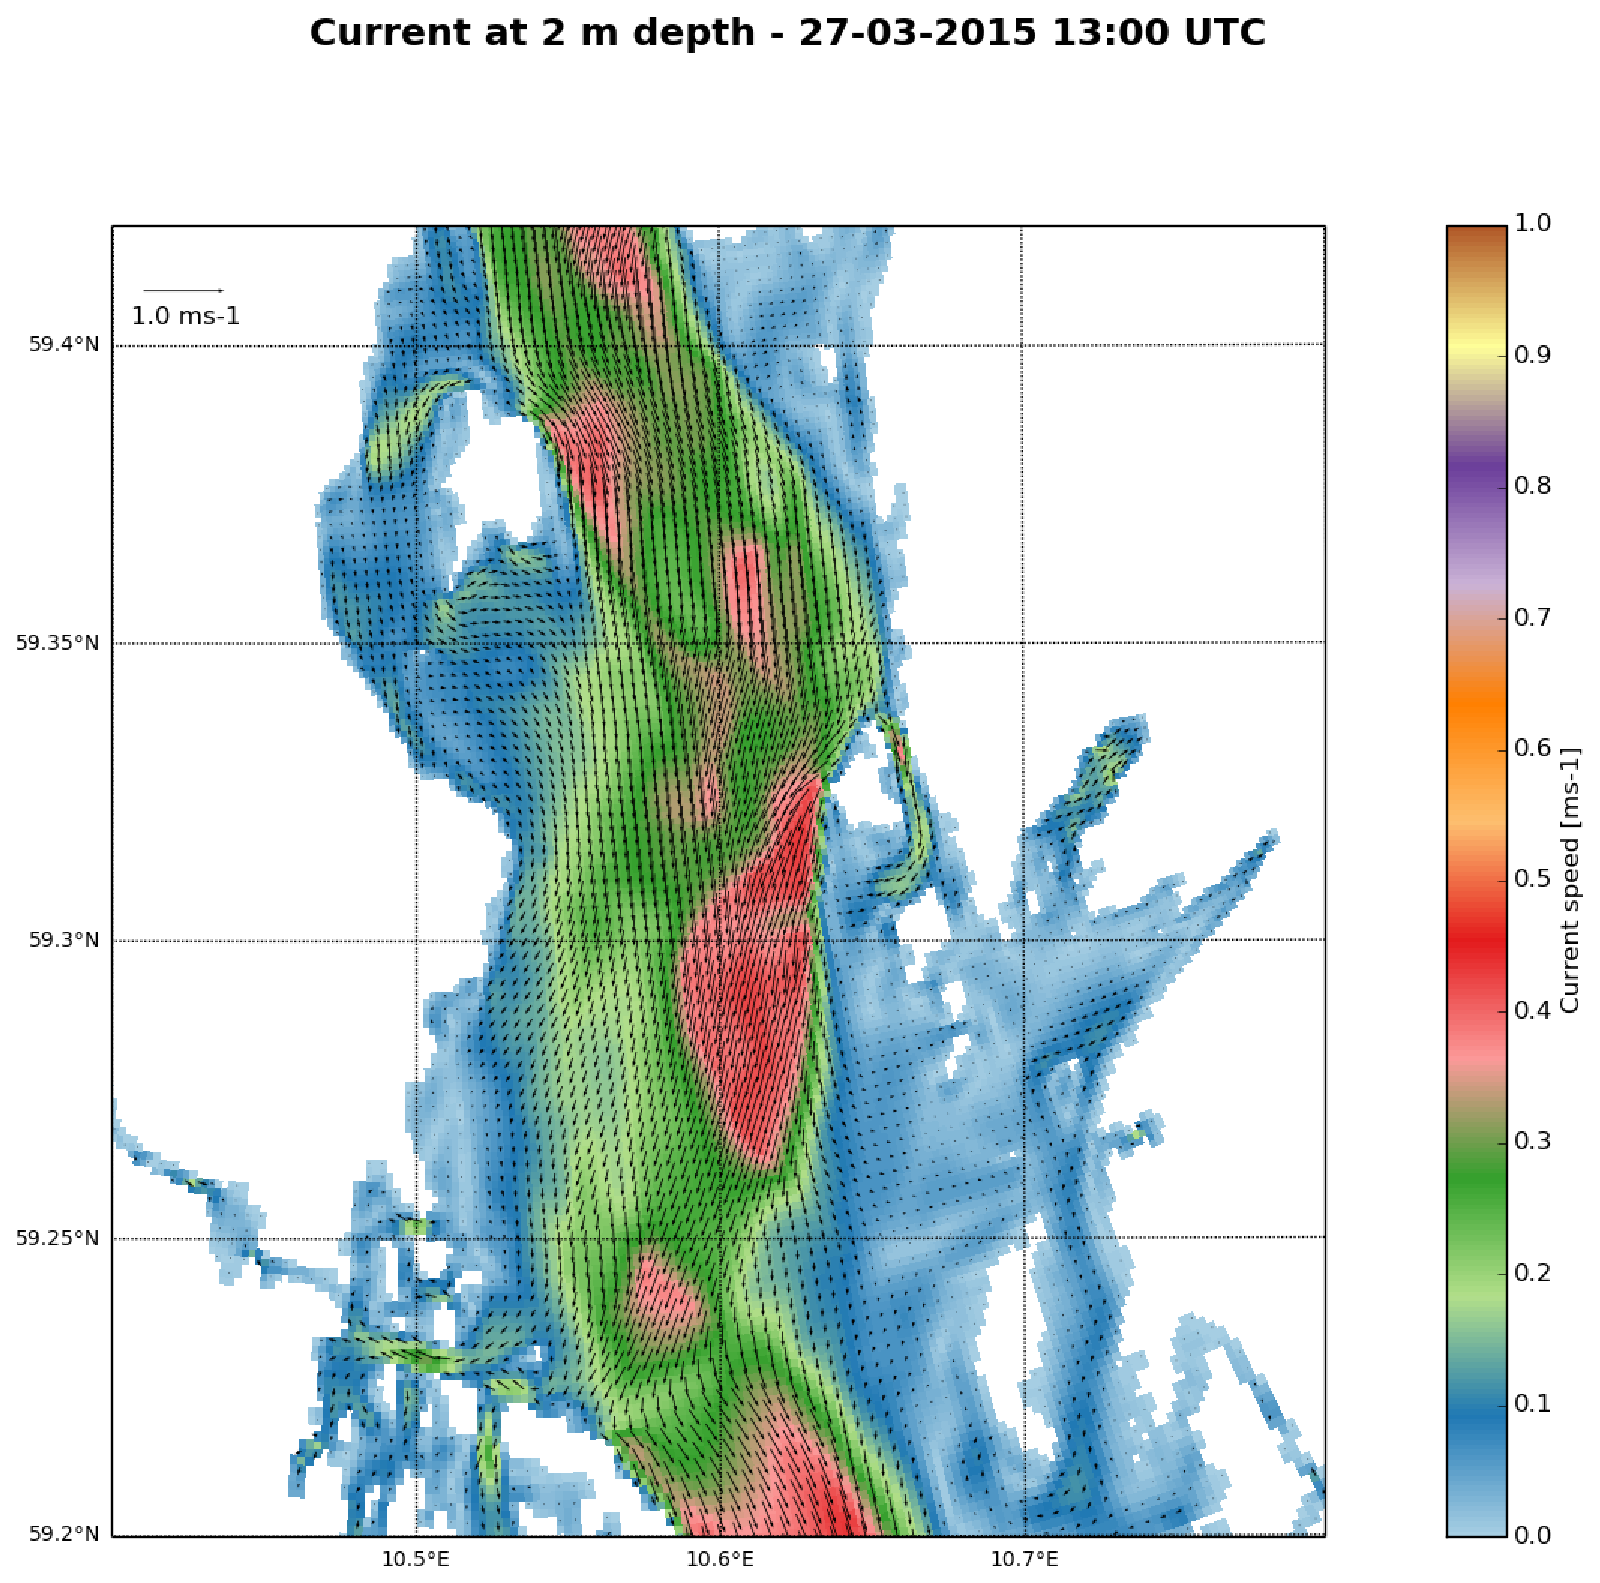
\includegraphics[height=16cm]{kap5/ferder4__0_current_crop}}
  \end{pspicture}
  \caption{\small  As Figure \ref{fig:curr_oslo}, but for the area between the Bast{\o}y, Rauer and Bol{\ae}rne islands.  }
  \label{fig:curr_mefjord}
\end{figure}

  
 %%%%%%%%%%%%%%%%%%% Figure  %%%%%%%%%%%%%%%
\begin{figure}[t]
  \begin{pspicture}(0,0)(15,12)
% Include graphs
	\rput[b](7.5,0){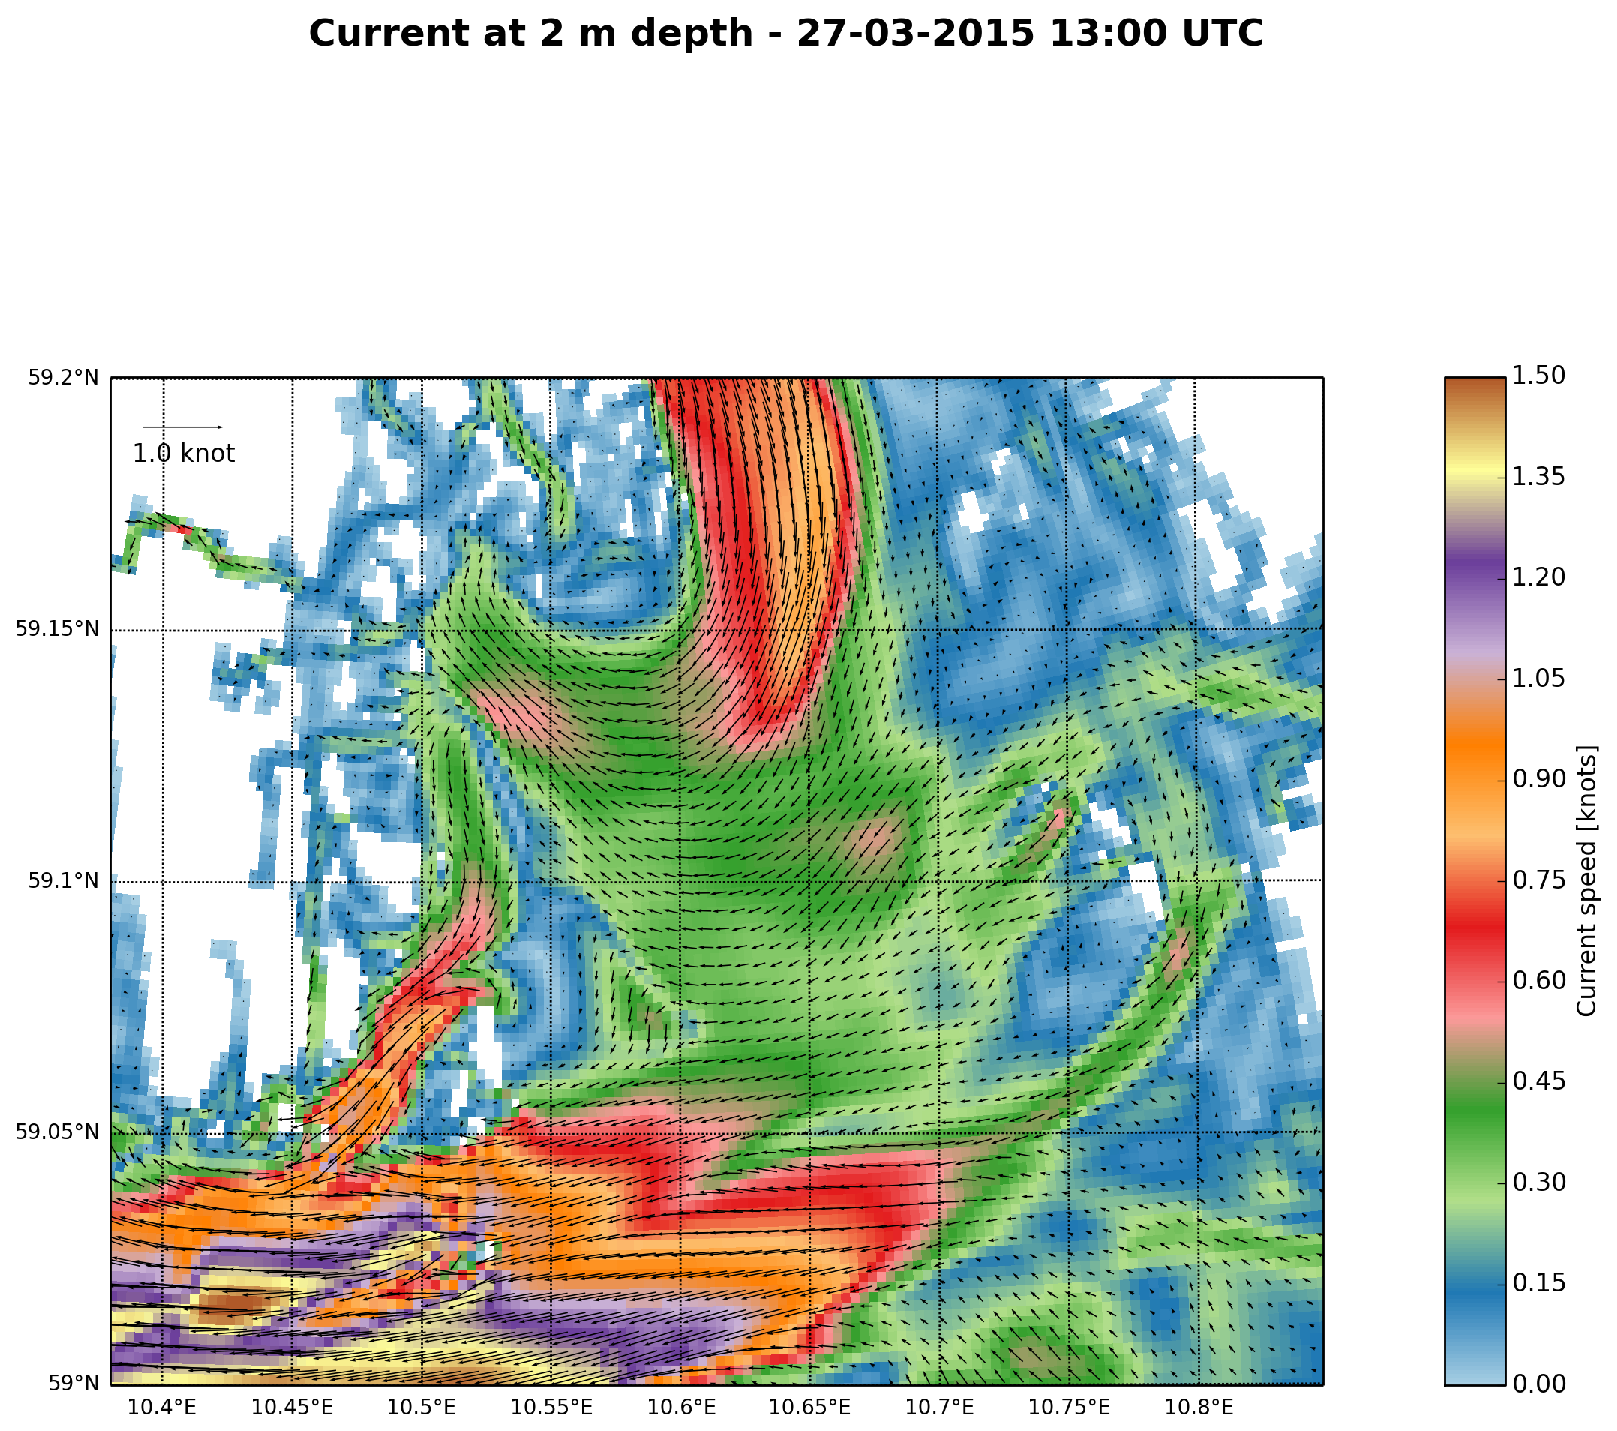
\includegraphics[height=12cm]{kap5/ferder5__0_current_crop}}
  \end{pspicture}
  \caption{\small  As for figure \ref{fig:curr_oslo}, but for the area around the F{\ae}rder lighthouse.  }
  \label{fig:curr_faerder}
\end{figure}

  
 %%%%%%%%%%%%%%%%%%% Figure  %%%%%%%%%%%%%%%
\begin{figure}[t]
  \begin{pspicture}(0,0)(15,16)
% Include graphs
	\rput[b](7.5,0){
\includegraphics[height=16cm]{kap5/drammen1__0_current_crop}}
  \end{pspicture}
  \caption{\small  As for figure \ref{fig:curr_oslo}, but for the Drammensfjord and western Breidangen area.  }
  \label{fig:curr_drammen}
\end{figure}

  

%\subsubsection{Temperature}
 %%%%%%%%%%%%%%%%%%% Figure  %%%%%%%%%%%%%%%
\begin{figure}[t]
  \begin{pspicture}(0,0)(15,12)
% Include graphs
	\rput[b](7.5,0){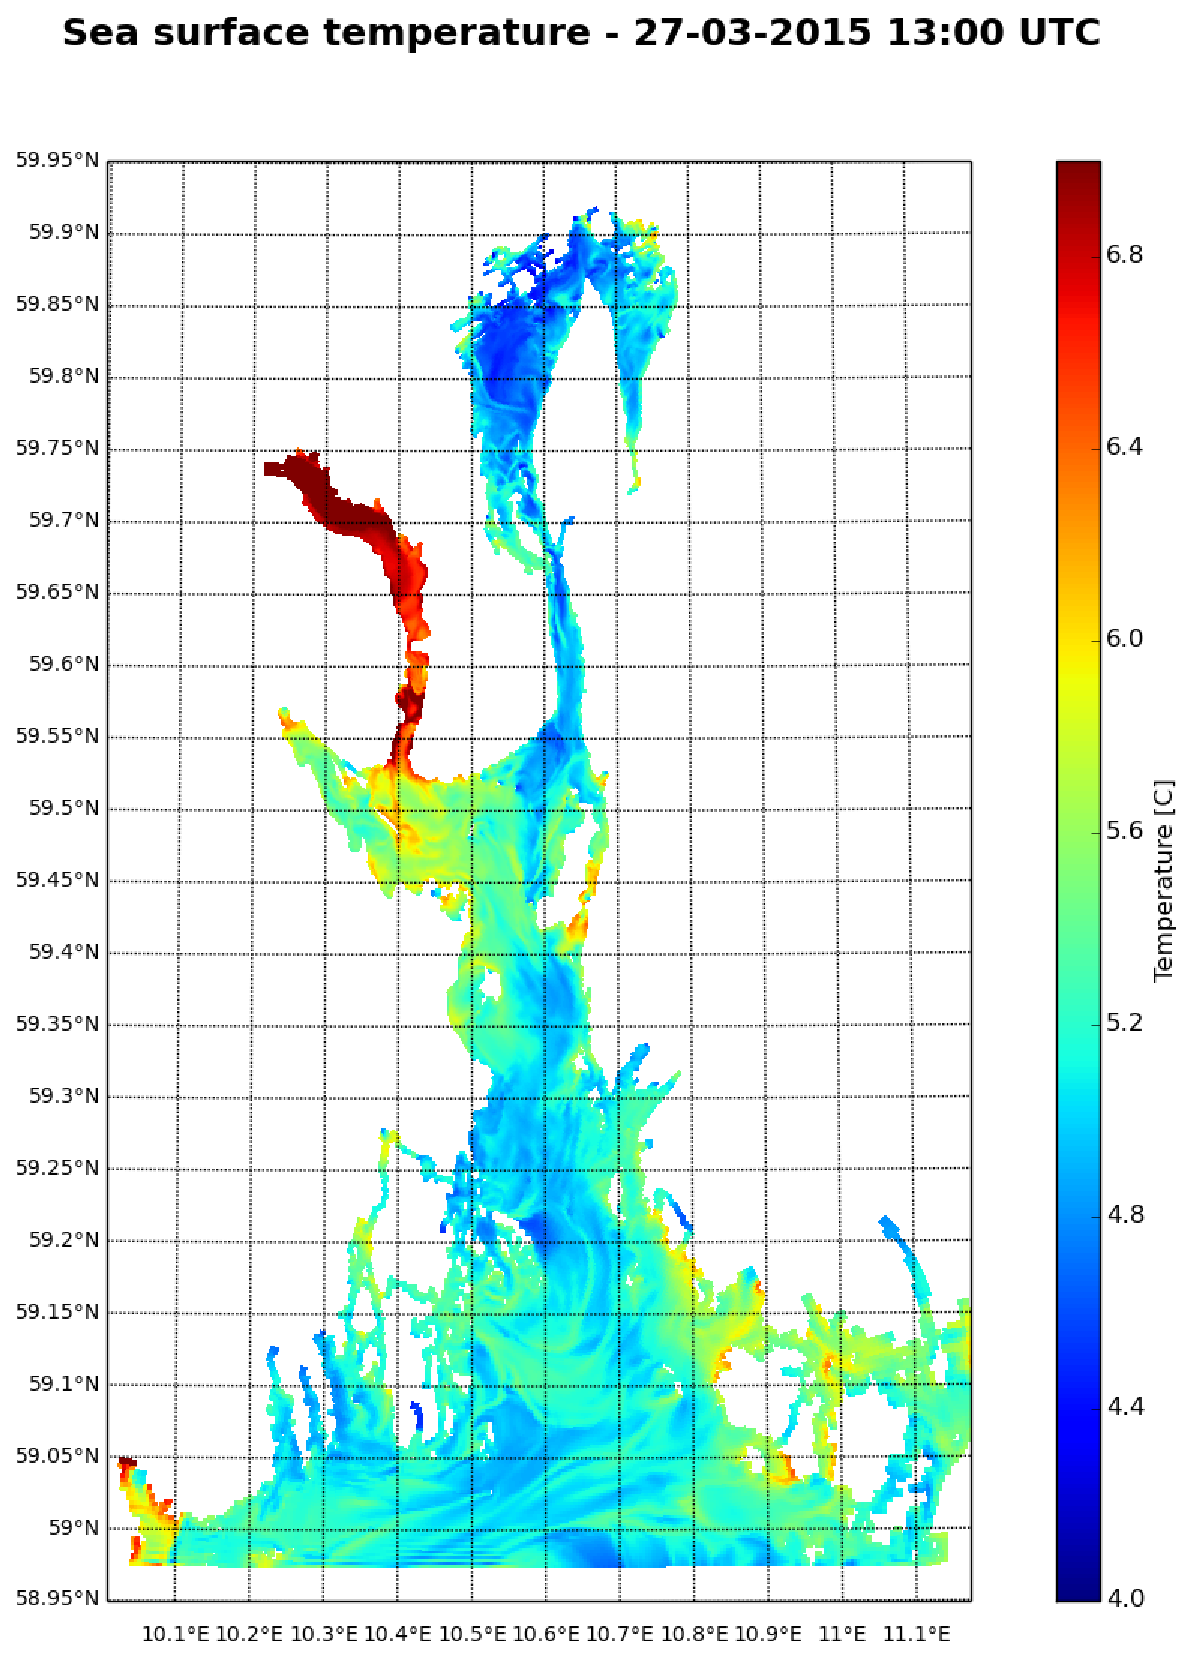
\includegraphics[height=12cm]{kap5/temp_hele_0_current_crop}}
  \end{pspicture}
  \caption{\small  Sea surface temperature (SST) for the entire model domain of the FjordOs model. Note the high SST in the Drammensfjorden area. We believe this is not realistic, and is most likely cause by the mixing up of warmer water from below. This warm water is probably left from imperfect initial conditions. }
  \label{fig:temp_hele}
\end{figure}

  

%\subsubsection{Salinity}
 %%%%%%%%%%%%%%%%%%% Figure  %%%%%%%%%%%%%%%
\begin{figure}[t]
  \begin{pspicture}(0,0)(15,12)
% Include graphs
	\rput[b](7.5,0){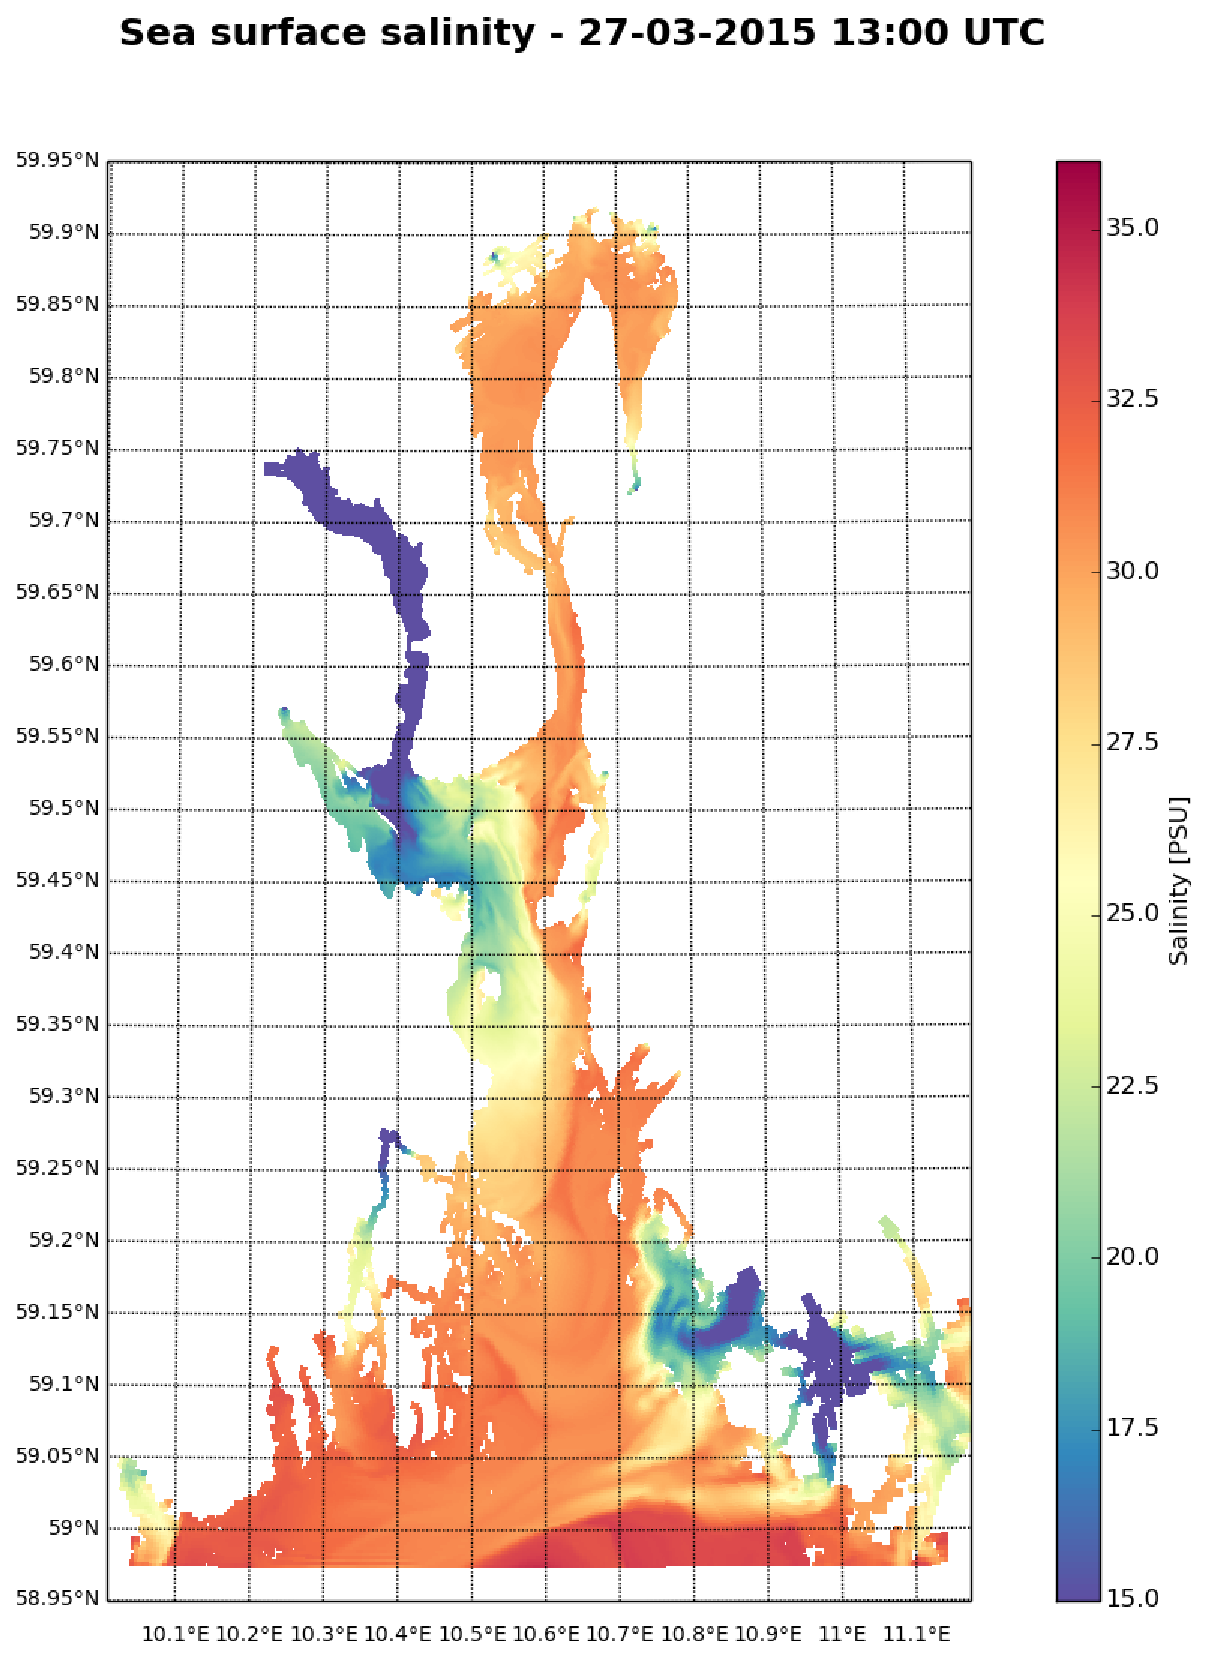
\includegraphics[height=12cm]{kap5/salt_hele_0_current_crop}}
  \end{pspicture}
  \caption{\small  As for figure \ref{fig:temp_hele}, but for sea surface salinity (SSS).  }
  \label{fig:salt_hele}
\end{figure}

  

%\subsubsection{Sea level}
 %%%%%%%%%%%%%%%%%%% Figure  %%%%%%%%%%%%%%%
\begin{figure}[t]
  \begin{pspicture}(0,0)(15,17)
% Include graphs
	\rput[b](7.5,0){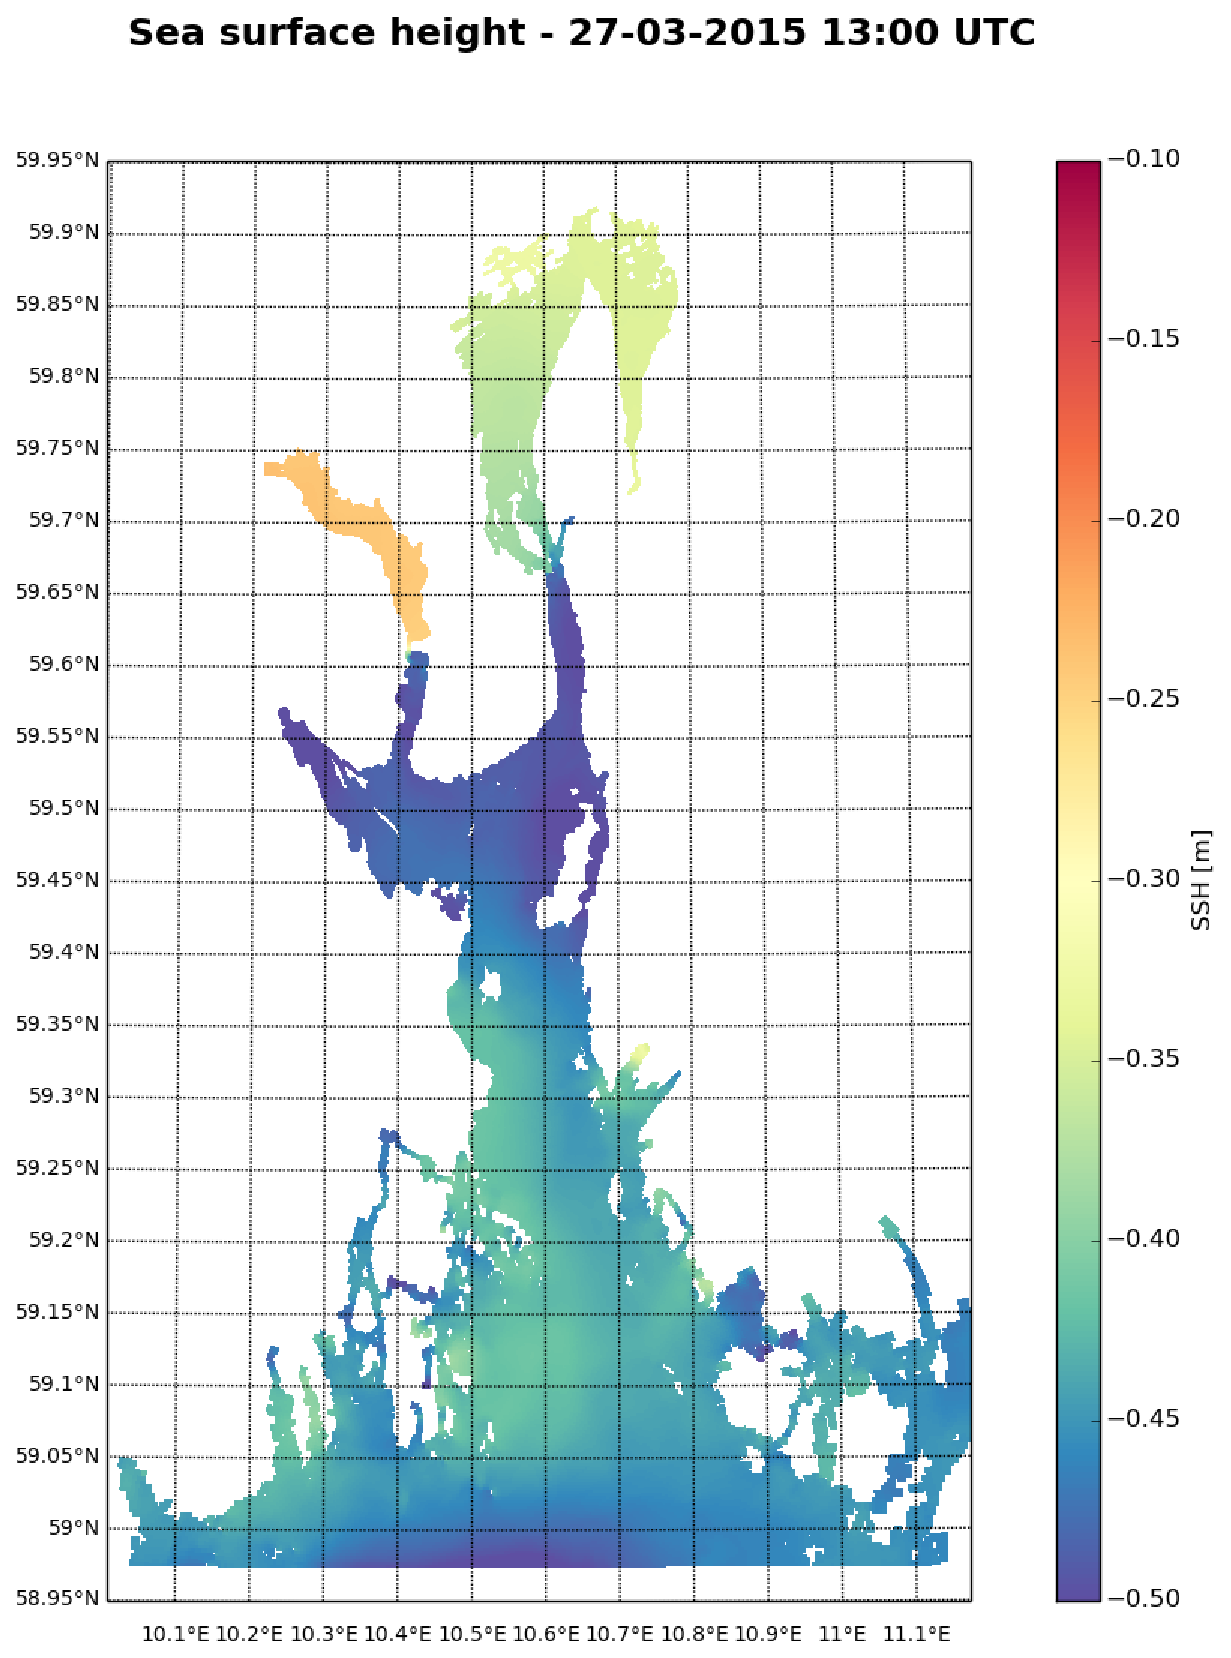
\includegraphics[height=17cm]{kap5/zeta_hele_0_crop}}
  \end{pspicture}
  \caption{\small  As for figure \ref{fig:temp_hele}, but for sea surface height (SSH).  }
  \label{fig:ssh_hele}
\end{figure}

  


% Example: figure
%\begin{figure}[ht]
%\centerline{
%a
%\resizebox{8.0cm}{8.0cm}{
%\includegraphics*{metno_7/RCM_TxTn_ta.a2-ta.cl.eps}}
%}
%\centerline{
%b
%\resizebox{8.0cm}{8.0cm}{
%\includegraphics*{metno_7/RCM_TxTn_oslo-months.eps}}
%}
%\caption{\small
%caption
%}
%\label{fig:X}
%\end{figure}

\newpage
\section{Summary and final remarks}
\label{sec:summa}
A documentation of a new Oslofjord model is provided. The new Oslofjord model, named FjordOs CL, is based on the publically available ocean model ROMS \citep{shche:mcwil:2005,shche:mcwil:2009,haidv:etal:2008}, and is developed as part of the project FjordOs. FjordOs CL exploits the curvilinear option in ROMS to minimize the number of ``dry'' grid points at the expense of increasing the number of ``wet'' grid points. Thereby the grid resolution is enhanced and varies in space. In fact the FjordOs CL mesh size varies from about 50 m in the {\DR} area to about 300 m at its southern border. 

To satisfy ourselves that the model works technically, is viable and produces results that are in line with our knowledge of the cirtculation in the fjord, we have run several test cases. Above we have shown examples of results from a hindcast case initiated on April 1, 2014 and run through December 31, 2015. A through validation of the sresults from this hindcast will be reported in a separete report.

In summary the results shown provides insight into the necessity of resolving the Oslofjord's irregular coastline geography, that is, the fjord's many small islands, narrow sounds and straigts, and its topography, that is, deep basins and shallow areas. Thus the new model provides a basis for developing an operation Oslofjord model once well identified and validated.


\clearpage
\section*{\hspace{17mm}Acknowledgements}
The present research and development is mostly funded by the the regional research funds Oslofjordfondet. We gratefully acknowledge the support. Smaller contributions from MET Norway, NIVA, HSN, Kystverket and Exxon are also appreciated. We would also like to thank Kai H. Christensen and Ann Kristin Sperrevik, both from MET Norway, for many helpful discussions and suggestions.   

%\clearpage
%\section*{\hspace{17mm}Appendix}


%\begin{table}[h]
%\vspace{-1.5cm}
%{\bf Table A1: ESD statistics.}\\
%\label{tab:1}
%\begin{tabular}{llll}
%\small OSLO - BLINDERN 18700 & 
%\small $T_m$ $R^2$= 71 -- 86 $T_x$ $R^2$= 69 -- 82 $T_n$ $R^2$= 49 -- 76 \\
%\small $\Delta T_m$ $q_{0.05}$= 3.21 $q_{0.50}$= 1.33 $q_{0.95}$= 1.75 \\  
%\small $\Delta T_x$ $q_{0.05}$= 3.09 $q_{0.50}$= 1.38 $q_{0.95}$= 2.16 \\  
%\small $\Delta T_n$ $q_{0.05}$= 3.15 $q_{0.50}$= 1.12 $q_{0.95}$= 1.01 \\
%\end{tabular}
%\end{table}

\clearpage
\pagebreak

%%%%%%%%%%%%%%%%%%%%%%%%%%%%%%%%%%%%%%%%%%%%%%%%%%%%%%%%%%%%%%%%%%%%%%%
% Specify path to where to find the citations (natbib)
\bibliography{referanse-lpr}
%\begin{thebibliography}{1}
%\end{thebibliography}

\clearpage
\pagebreak
 

\end{document}
